\documentclass[final,paperwidth=36in,paperheight=48in,portrait,fontscale=0.3]{baposter}
% NIPS Workshops format

% Encoding.
\usepackage[utf8]{inputenc}
\usepackage[T1]{fontenc}

\usepackage{graphicx} % Required for including images
\usepackage{subfig}
\usepackage{booktabs} % for professional tables
\usepackage{floatrow}
\usepackage{float}

\usepackage{textgreek}
\usepackage{pstricks}
\usepackage{tikz}
\usepackage{pgf}
\usepackage{placeins} % For \FloatBarrier
\usetikzlibrary{positioning}
\usepackage{environ}
\makeatletter
\newsavebox{\measure@tikzpicture}
\NewEnviron{scaletikzpicturetowidth}[1]{%
	\def\tikz@width{#1}%
	\def\tikzscale{1}\begin{lrbox}{\measure@tikzpicture}%
		\BODY
	\end{lrbox}%
	\pgfmathparse{#1/\wd\measure@tikzpicture}%
	\edef\tikzscale{\pgfmathresult}%
	\BODY
}
\makeatother

\usepackage{amsmath} % For typesetting math
\usepackage{amssymb} % Adds new symbols to be used in math mode

\usepackage{booktabs} % Top and bottom rules for tables
\usepackage{enumitem} % Used to reduce itemize/enumerate spacing
%\usepackage{palatino} % Use the Palatino font
\renewcommand{\familydefault}{\sfdefault}
\usepackage[font=small,labelfont=bf]{caption} % Required for specifying captions to tables and figures

\usepackage{multicol} % Required for multiple columns
\setlength{\columnsep}{1.5em} % Slightly increase the space between columns
\setlength{\columnseprule}{0mm} % No horizontal rule between columns
\usepackage{multirow}


\newcommand{\compresslist}{ % Define a command to reduce spacing within itemize/enumerate environments, this is used right after \begin{itemize} or \begin{enumerate}
\setlength{\itemsep}{1pt}
\setlength{\parskip}{0pt}
\setlength{\parsep}{0pt}
}

% Defines the color used for content box headers
\definecolor{lightblue}{cmyk}{0.83,0.24,0,0.16}
%\definecolor{lightblue}{rgb}{0.145,0.6666,1}

%%%%%%%%%%%%%%%%%%%%%%%%%%%%%%%%%%%%%%%%%%%%%%%%%%%%%%%%%%%%%%%%%%%%%%%%%%%%%%
%%% Begin of Document
%%%%%%%%%%%%%%%%%%%%%%%%%%%%%%%%%%%%%%%%%%%%%%%%%%%%%%%%%%%%%%%%%%%%%%%%%%%%%%

% Pojedyncze spacje po kropce.
\frenchspacing

\begin{document}



\hyphenation{resolution occlusions}
%%
\begin{poster}%
  % Poster Options
  {
  % Show grid to help with alignment
  grid=false,
  % Column spacing
  colspacing=1em,
  % Color style
  bgColorOne=white,
  bgColorTwo=white,
  borderColor=lightblue,
  headerColorOne=black,
  headerColorTwo=lightblue,
  headerFontColor=white,
  boxColorOne=white,
  boxColorTwo=lightblue,
  % Format of textbox
  textborder=roundedleft,
%  textborder=faded,
  % Format of text header
  eyecatcher=true,
  headerborder=closed,
  columns=2,
  headerheight=4cm,
%  textfont=\sc, An example of changing the text font
  headershape=roundedright,
  headershade=shadelr,
  headerfont=\Large\bf\textsc, %Sans Serif
  textfont={\setlength{\parindent}{1.5em}\large},
  boxshade=plain,
%  background=shade-tb,
  background=plain,
  linewidth=1pt
  } 
  { % Left Eye Catcher - IBM logo

\includegraphics[width=4cm]{../img/ibm_research.png}
  } 
  % Title
  	{\bf\textsc{Learning Beyond Simulated Physics}\vspace{0.2em}}
  % Authors
  {
	\textbf{Alexis Asseman, Tomasz Kornuta, Ahmet S. Ozcan}\\
	IBM Research AI, Almaden Research Center, San Jose, USA\\
	\texttt{alexis.asseman@ibm.com}, \texttt{\{tkornut, asozcan\}@us.ibm.com}\\
  }
  { % Left Eye Catcher

\includegraphics[width=4cm]{../img/arc_logo.png}
  }


% A coloured circle useful as a bullet with an adjustably strong filling
\newcommand{\colouredcircle}{%
\tikz{\useasboundingbox (-0.2em,-0.32em) rectangle(0.2em,0.32em); \draw[draw=black,fill=lightblue,line width=0.03em] (0,0) circle(0.16em);}}
\tikzstyle{block} = [draw,minimum size=2.5em, outer sep=2]

%%%%%%%%%%%%%%%%%%%%%%%%%%%%%%%%%%%%%%%%%%%%%%%%%%%%%%%%%%%%%%%%%%%%%%%%%%%%%%%

\headerbox{Abstract}{name=abstract,column=0,row=0}{
	Most advancements in terms of \textbf{time-series predictions of physical systems} is based on simulated physics.
	Thus we are proposing a \textbf{new dataset} based on videos of a real-world, \textbf{chaotic double pendulum}.
	We show baseline performance using an LSTM model, demonstrating the possibility of training directly on a real physical system.
} %headerbox

\headerbox{The Double Pendulum}{name=double-pendulum, column=0, below=abstract}{
	\begin{figure}[H]
		\centering
		\subfloat[]{{
				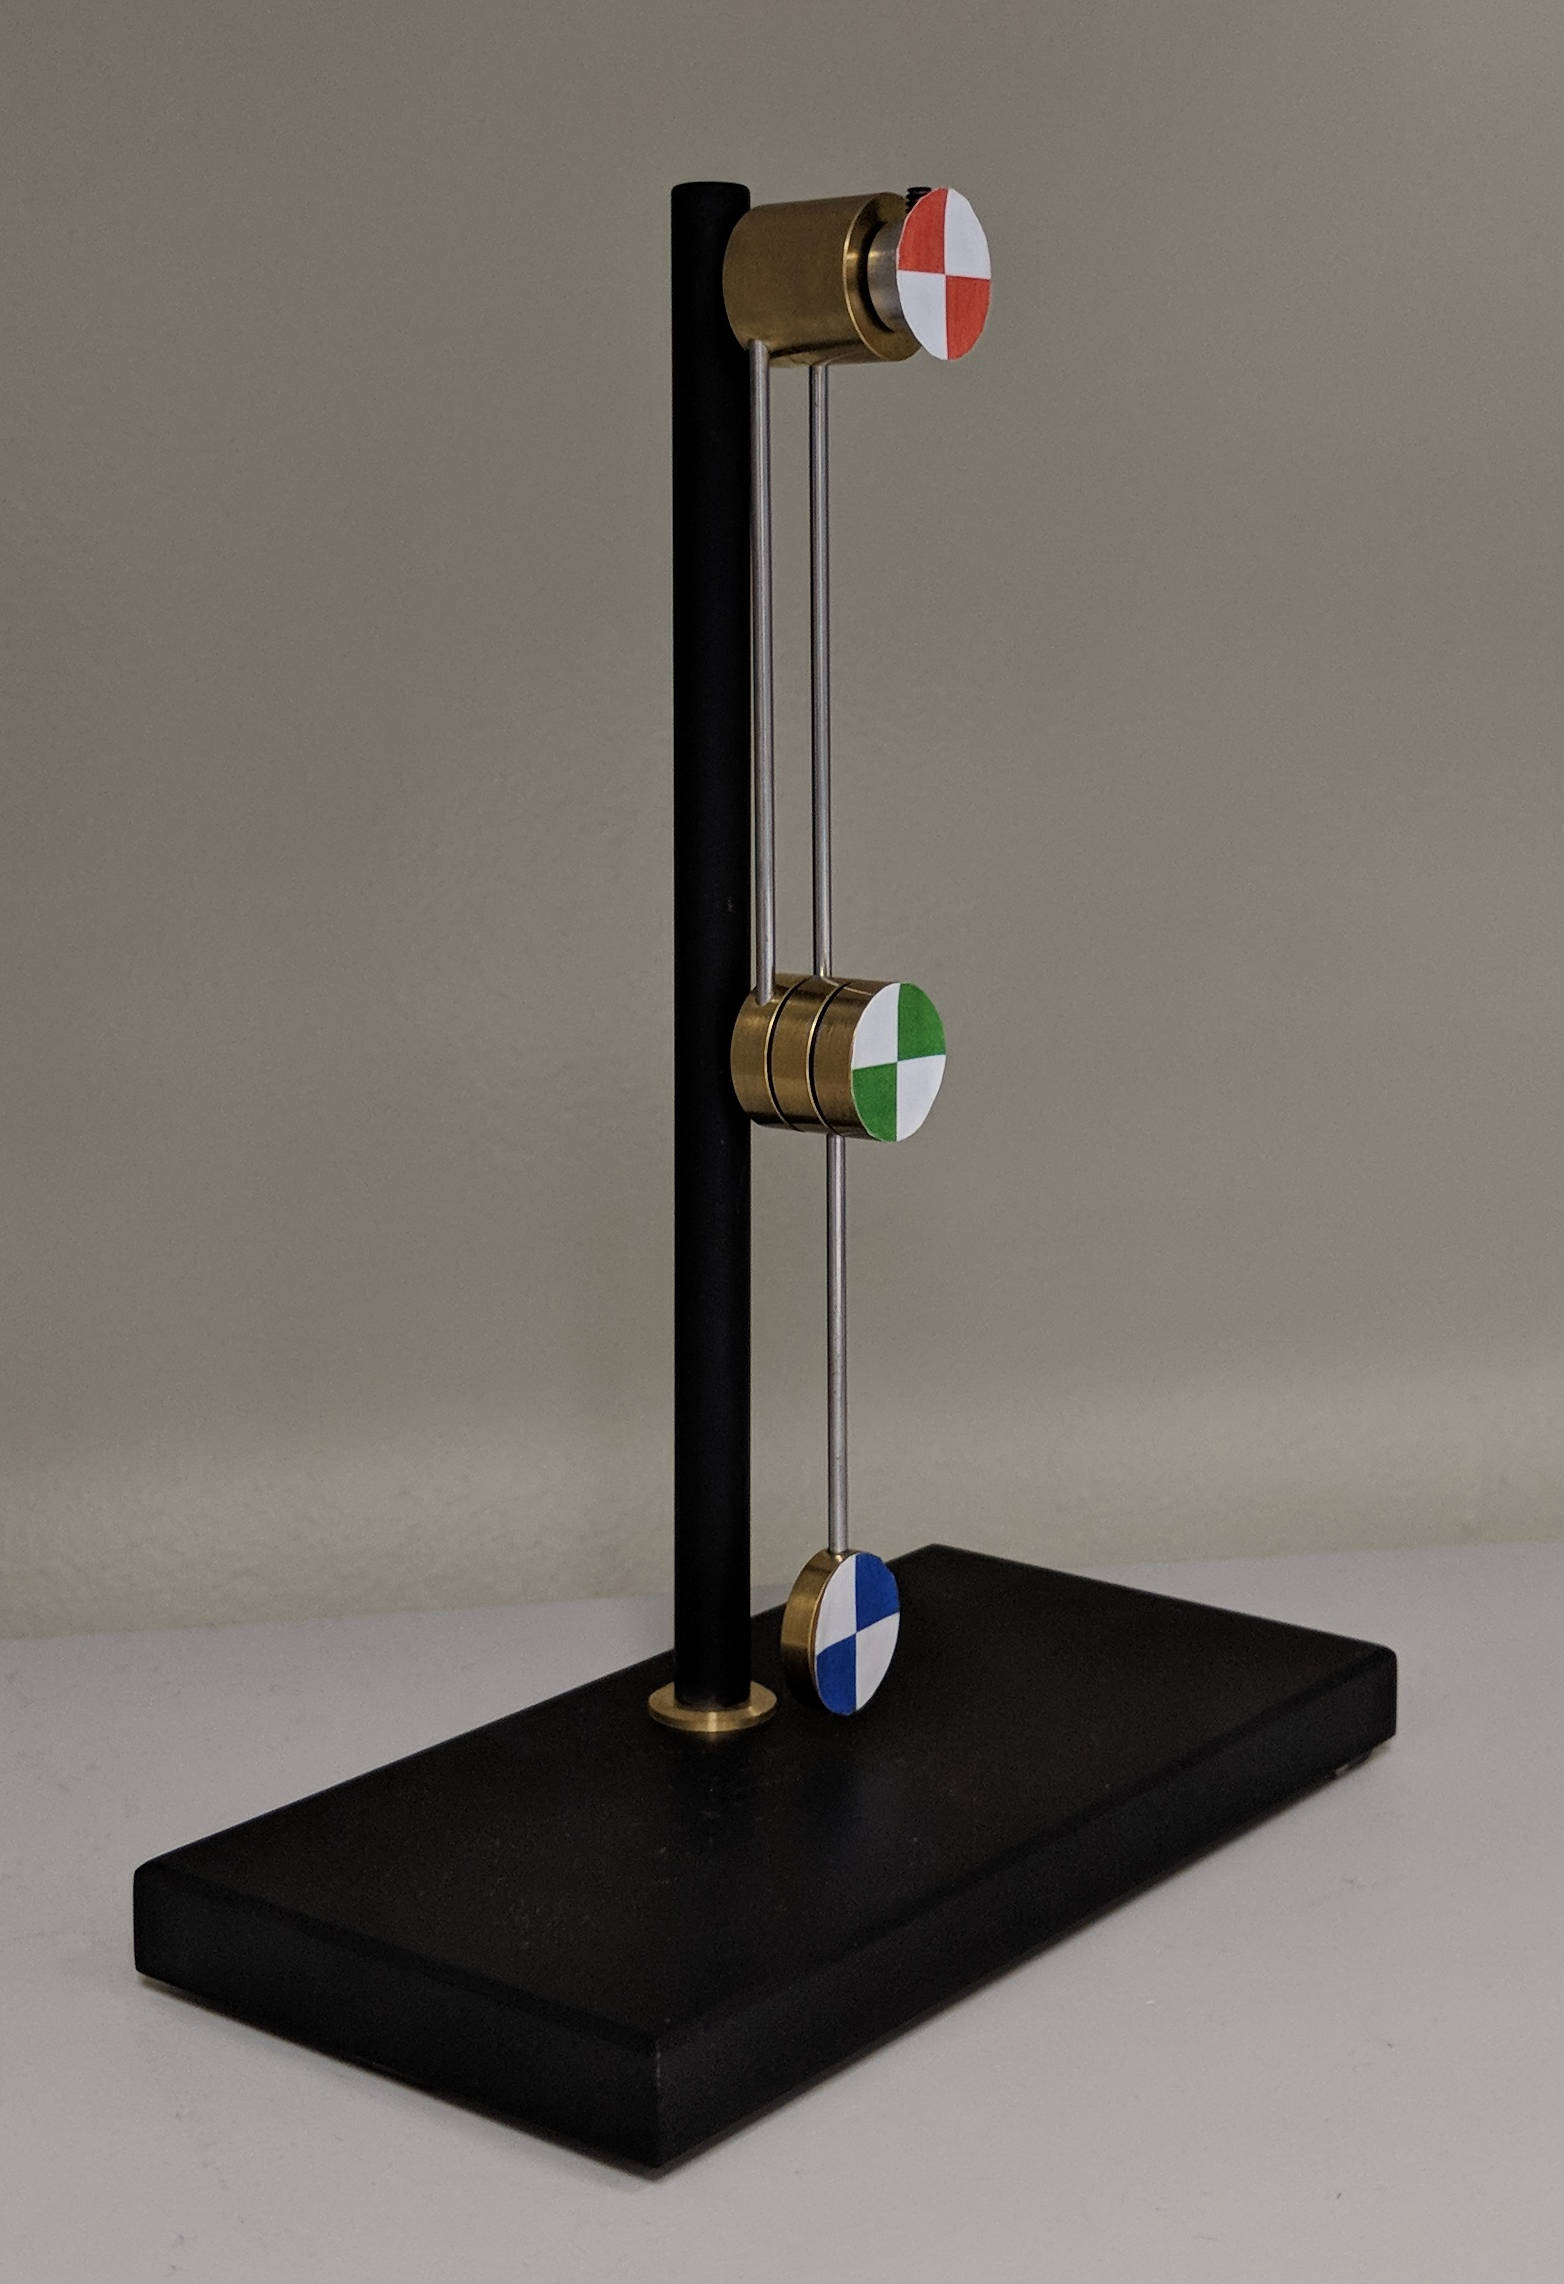
\includegraphics[width=0.27\textwidth]{../img/pendulum.jpg}
				\label{subfig:pendulum_picture}
		}}
		\quad\quad\quad
		\subfloat[]{{
				\def\svgwidth{0.3\textwidth}
				\footnotesize
				\input{../img/pendulum_dimensions.pdf_tex}
				\label{subfig:pendulum_dimensions}
		}}
		\caption{A picture \ref{subfig:pendulum_picture} and the dimensions \ref{subfig:pendulum_dimensions} of the double pendulum.}
		\label{fig:pendulum}
	\end{figure}
	
	The double pendulum is a \textbf{chaotic}\cite{levien1993} mechanical device. Even though it can be simulated, we chose to use a real one to create the Double Pendulum Chaotic Dataset. The behavior of the pendulum is influenced by environmental noise, i.e. air motion, coupling with the table, imperfections of the device, etc.
}

\headerbox{Data Acquisition}{name=data acquisition, column=0, below=double-pendulum}{
	\begin{figure}[H]
		\centering
		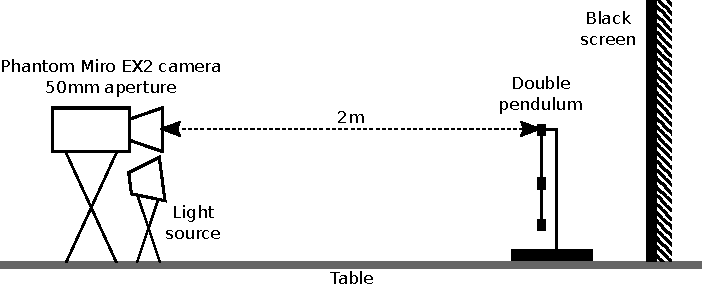
\includegraphics[width=0.8\textwidth]{../img/camera_set_up.pdf}
		\caption{Camera set-up.}
		\label{fig:camera_set_up}
	\end{figure}
	\begin{table}[H]
		\centering
		\caption{Summary of the video settings}
		\begin{tabular}{ll}
			\toprule
			\multicolumn{2}{c}{Camera settings}\\
			\cmidrule{1-2}
			Resolution & 480x480 pixels\\
			Capture frame-rate & 400 Hz\\
			Frame exposure time & 90 \textmu s\\
			\cmidrule{1-2}
			\multicolumn{2}{c}{Data properties}\\
			\cmidrule{1-2}
			Sequence capture duration & $\approx$ 40 s\\
			Number of frames per sequence & $\approx$ 17500\\
			Number of sequences & 21\\
			\bottomrule
		\end{tabular}
		\label{tab:data_properties}
	\end{table}
	\begin{figure}[H]
		\centering
		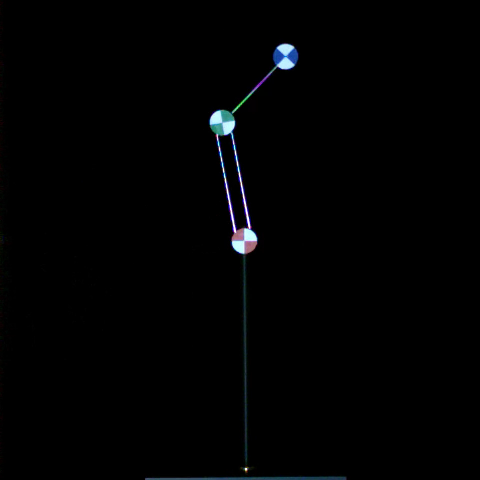
\includegraphics[width=0.25\textwidth]{../img/0100.png}
		\caption{A video frame.}
		\label{fig:video_frame}
	\end{figure}
}

\headerbox{The Dataset}{name=dataset, column=1}{
	The dataset is available as:
	\vspace{-4pt}
	\begin{itemize}
		\itemsep0em 
		\item Full length, high quality videos
		\item Corresponding CSV files of the positions through time
	\end{itemize}
	And the ones above, precut as a train/test dataset, such that:
	\begin{figure}[H]
		\centering
		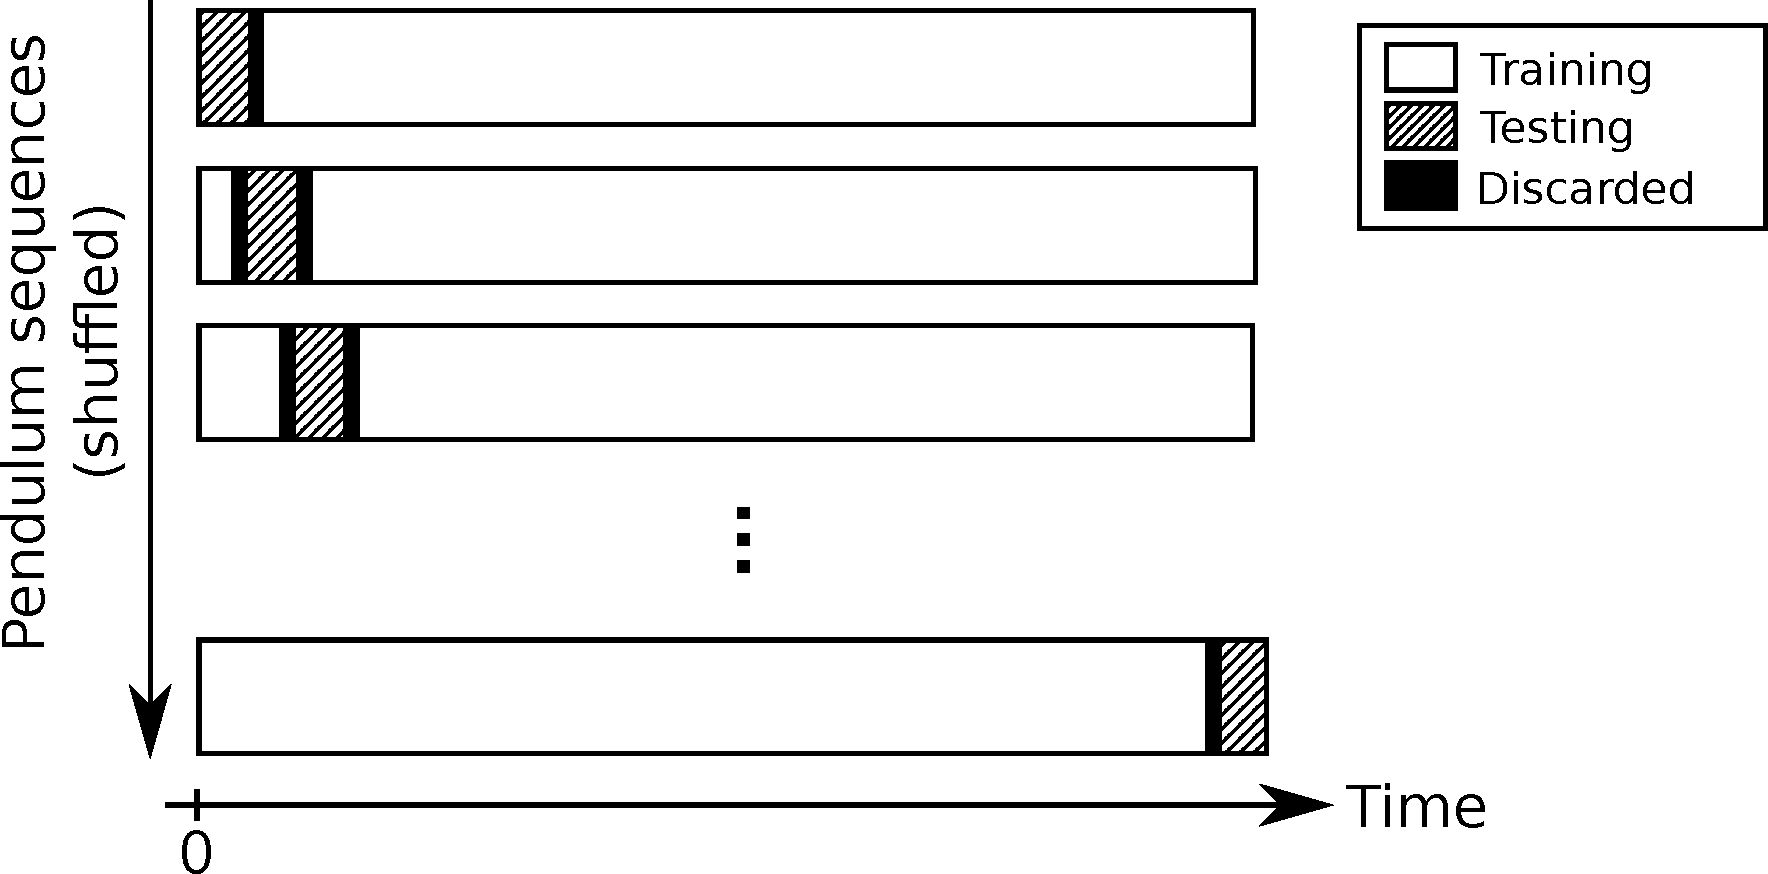
\includegraphics[width=0.7\textwidth]{../img/dataset_split_2.pdf}
		\caption{Split of the dataset (To scale).}
		\label{fig:dataset_split}
	\end{figure}
	\vspace{-4pt}
	Where the testing data is cut in sequences of \textbf{4 input frames and 200 prediction ground-truth frames}.
}

\headerbox{ML baseline with LSTM}{name=baseline, column=1, below=dataset}{
	{
	\begin{minipage}[H]{0.4\textwidth}
		\begin{figure}[H]
			\centering
			\caption{Diagram of the LSTM\cite{lstm-paper}-based recurrent neural network used. It takes one time-step as input and predicts the next one.}
			\label{fig:lstm_diag}
			\small
			\def\svgwidth{4cm}
			\input{../img/lstm.pdf_tex}
		\end{figure}
	\end{minipage}
	\hfill
	\begin{minipage}[H]{0.4\textwidth}
		\begin{figure}[H]
			\centering
			\scalebox{0.72}{%% Creator: Matplotlib, PGF backend
%%
%% To include the figure in your LaTeX document, write
%%   \input{<filename>.pgf}
%%
%% Make sure the required packages are loaded in your preamble
%%   \usepackage{pgf}
%%
%% Figures using additional raster images can only be included by \input if
%% they are in the same directory as the main LaTeX file. For loading figures
%% from other directories you can use the `import` package
%%   \usepackage{import}
%% and then include the figures with
%%   \import{<path to file>}{<filename>.pgf}
%%
%% Matplotlib used the following preamble
%%   \usepackage[utf8x]{inputenc}
%%   \usepackage[T1]{fontenc}
%%
\begingroup%
\makeatletter%
\begin{pgfpicture}%
\pgfpathrectangle{\pgfpointorigin}{\pgfqpoint{3.180034in}{3.071806in}}%
\pgfusepath{use as bounding box, clip}%
\begin{pgfscope}%
\pgfsetbuttcap%
\pgfsetmiterjoin%
\definecolor{currentfill}{rgb}{1.000000,1.000000,1.000000}%
\pgfsetfillcolor{currentfill}%
\pgfsetlinewidth{0.000000pt}%
\definecolor{currentstroke}{rgb}{1.000000,1.000000,1.000000}%
\pgfsetstrokecolor{currentstroke}%
\pgfsetdash{}{0pt}%
\pgfpathmoveto{\pgfqpoint{0.000000in}{0.000000in}}%
\pgfpathlineto{\pgfqpoint{3.180034in}{0.000000in}}%
\pgfpathlineto{\pgfqpoint{3.180034in}{3.071806in}}%
\pgfpathlineto{\pgfqpoint{0.000000in}{3.071806in}}%
\pgfpathclose%
\pgfusepath{fill}%
\end{pgfscope}%
\begin{pgfscope}%
\pgfsetbuttcap%
\pgfsetmiterjoin%
\definecolor{currentfill}{rgb}{1.000000,1.000000,1.000000}%
\pgfsetfillcolor{currentfill}%
\pgfsetlinewidth{0.000000pt}%
\definecolor{currentstroke}{rgb}{0.000000,0.000000,0.000000}%
\pgfsetstrokecolor{currentstroke}%
\pgfsetstrokeopacity{0.000000}%
\pgfsetdash{}{0pt}%
\pgfpathmoveto{\pgfqpoint{0.526284in}{1.370043in}}%
\pgfpathlineto{\pgfqpoint{1.735659in}{1.370043in}}%
\pgfpathlineto{\pgfqpoint{1.735659in}{2.166529in}}%
\pgfpathlineto{\pgfqpoint{0.526284in}{2.166529in}}%
\pgfpathclose%
\pgfusepath{fill}%
\end{pgfscope}%
\begin{pgfscope}%
\pgfsetbuttcap%
\pgfsetroundjoin%
\definecolor{currentfill}{rgb}{0.000000,0.000000,0.000000}%
\pgfsetfillcolor{currentfill}%
\pgfsetlinewidth{0.803000pt}%
\definecolor{currentstroke}{rgb}{0.000000,0.000000,0.000000}%
\pgfsetstrokecolor{currentstroke}%
\pgfsetdash{}{0pt}%
\pgfsys@defobject{currentmarker}{\pgfqpoint{0.000000in}{-0.048611in}}{\pgfqpoint{0.000000in}{0.000000in}}{%
\pgfpathmoveto{\pgfqpoint{0.000000in}{0.000000in}}%
\pgfpathlineto{\pgfqpoint{0.000000in}{-0.048611in}}%
\pgfusepath{stroke,fill}%
}%
\begin{pgfscope}%
\pgfsys@transformshift{0.580274in}{1.370043in}%
\pgfsys@useobject{currentmarker}{}%
\end{pgfscope}%
\end{pgfscope}%
\begin{pgfscope}%
\pgfsetbuttcap%
\pgfsetroundjoin%
\definecolor{currentfill}{rgb}{0.000000,0.000000,0.000000}%
\pgfsetfillcolor{currentfill}%
\pgfsetlinewidth{0.803000pt}%
\definecolor{currentstroke}{rgb}{0.000000,0.000000,0.000000}%
\pgfsetstrokecolor{currentstroke}%
\pgfsetdash{}{0pt}%
\pgfsys@defobject{currentmarker}{\pgfqpoint{0.000000in}{-0.048611in}}{\pgfqpoint{0.000000in}{0.000000in}}{%
\pgfpathmoveto{\pgfqpoint{0.000000in}{0.000000in}}%
\pgfpathlineto{\pgfqpoint{0.000000in}{-0.048611in}}%
\pgfusepath{stroke,fill}%
}%
\begin{pgfscope}%
\pgfsys@transformshift{1.120173in}{1.370043in}%
\pgfsys@useobject{currentmarker}{}%
\end{pgfscope}%
\end{pgfscope}%
\begin{pgfscope}%
\pgfsetbuttcap%
\pgfsetroundjoin%
\definecolor{currentfill}{rgb}{0.000000,0.000000,0.000000}%
\pgfsetfillcolor{currentfill}%
\pgfsetlinewidth{0.803000pt}%
\definecolor{currentstroke}{rgb}{0.000000,0.000000,0.000000}%
\pgfsetstrokecolor{currentstroke}%
\pgfsetdash{}{0pt}%
\pgfsys@defobject{currentmarker}{\pgfqpoint{0.000000in}{-0.048611in}}{\pgfqpoint{0.000000in}{0.000000in}}{%
\pgfpathmoveto{\pgfqpoint{0.000000in}{0.000000in}}%
\pgfpathlineto{\pgfqpoint{0.000000in}{-0.048611in}}%
\pgfusepath{stroke,fill}%
}%
\begin{pgfscope}%
\pgfsys@transformshift{1.660073in}{1.370043in}%
\pgfsys@useobject{currentmarker}{}%
\end{pgfscope}%
\end{pgfscope}%
\begin{pgfscope}%
\pgfsetbuttcap%
\pgfsetroundjoin%
\definecolor{currentfill}{rgb}{0.000000,0.000000,0.000000}%
\pgfsetfillcolor{currentfill}%
\pgfsetlinewidth{0.803000pt}%
\definecolor{currentstroke}{rgb}{0.000000,0.000000,0.000000}%
\pgfsetstrokecolor{currentstroke}%
\pgfsetdash{}{0pt}%
\pgfsys@defobject{currentmarker}{\pgfqpoint{-0.048611in}{0.000000in}}{\pgfqpoint{0.000000in}{0.000000in}}{%
\pgfpathmoveto{\pgfqpoint{0.000000in}{0.000000in}}%
\pgfpathlineto{\pgfqpoint{-0.048611in}{0.000000in}}%
\pgfusepath{stroke,fill}%
}%
\begin{pgfscope}%
\pgfsys@transformshift{0.526284in}{1.461945in}%
\pgfsys@useobject{currentmarker}{}%
\end{pgfscope}%
\end{pgfscope}%
\begin{pgfscope}%
\pgftext[x=0.278211in,y=1.423683in,left,base]{\rmfamily\fontsize{8.000000}{9.600000}\selectfont \(\displaystyle -1\)}%
\end{pgfscope}%
\begin{pgfscope}%
\pgfsetbuttcap%
\pgfsetroundjoin%
\definecolor{currentfill}{rgb}{0.000000,0.000000,0.000000}%
\pgfsetfillcolor{currentfill}%
\pgfsetlinewidth{0.803000pt}%
\definecolor{currentstroke}{rgb}{0.000000,0.000000,0.000000}%
\pgfsetstrokecolor{currentstroke}%
\pgfsetdash{}{0pt}%
\pgfsys@defobject{currentmarker}{\pgfqpoint{-0.048611in}{0.000000in}}{\pgfqpoint{0.000000in}{0.000000in}}{%
\pgfpathmoveto{\pgfqpoint{0.000000in}{0.000000in}}%
\pgfpathlineto{\pgfqpoint{-0.048611in}{0.000000in}}%
\pgfusepath{stroke,fill}%
}%
\begin{pgfscope}%
\pgfsys@transformshift{0.526284in}{1.768286in}%
\pgfsys@useobject{currentmarker}{}%
\end{pgfscope}%
\end{pgfscope}%
\begin{pgfscope}%
\pgftext[x=0.370033in,y=1.730024in,left,base]{\rmfamily\fontsize{8.000000}{9.600000}\selectfont \(\displaystyle 0\)}%
\end{pgfscope}%
\begin{pgfscope}%
\pgfsetbuttcap%
\pgfsetroundjoin%
\definecolor{currentfill}{rgb}{0.000000,0.000000,0.000000}%
\pgfsetfillcolor{currentfill}%
\pgfsetlinewidth{0.803000pt}%
\definecolor{currentstroke}{rgb}{0.000000,0.000000,0.000000}%
\pgfsetstrokecolor{currentstroke}%
\pgfsetdash{}{0pt}%
\pgfsys@defobject{currentmarker}{\pgfqpoint{-0.048611in}{0.000000in}}{\pgfqpoint{0.000000in}{0.000000in}}{%
\pgfpathmoveto{\pgfqpoint{0.000000in}{0.000000in}}%
\pgfpathlineto{\pgfqpoint{-0.048611in}{0.000000in}}%
\pgfusepath{stroke,fill}%
}%
\begin{pgfscope}%
\pgfsys@transformshift{0.526284in}{2.074627in}%
\pgfsys@useobject{currentmarker}{}%
\end{pgfscope}%
\end{pgfscope}%
\begin{pgfscope}%
\pgftext[x=0.370033in,y=2.036364in,left,base]{\rmfamily\fontsize{8.000000}{9.600000}\selectfont \(\displaystyle 1\)}%
\end{pgfscope}%
\begin{pgfscope}%
\pgftext[x=0.222655in,y=1.768286in,,bottom,rotate=90.000000]{\rmfamily\fontsize{10.000000}{12.000000}\selectfont Cosine}%
\end{pgfscope}%
\begin{pgfscope}%
\pgfpathrectangle{\pgfqpoint{0.526284in}{1.370043in}}{\pgfqpoint{1.209375in}{0.796486in}} %
\pgfusepath{clip}%
\pgfsetbuttcap%
\pgfsetroundjoin%
\pgfsetlinewidth{0.702625pt}%
\definecolor{currentstroke}{rgb}{0.000000,0.501961,0.000000}%
\pgfsetstrokecolor{currentstroke}%
\pgfsetdash{{0.700000pt}{1.155000pt}}{0.000000pt}%
\pgfpathmoveto{\pgfqpoint{0.596471in}{1.775080in}}%
\pgfpathlineto{\pgfqpoint{0.612668in}{1.783428in}}%
\pgfpathlineto{\pgfqpoint{0.623466in}{1.789148in}}%
\pgfpathlineto{\pgfqpoint{0.661259in}{1.815769in}}%
\pgfpathlineto{\pgfqpoint{0.693653in}{1.847478in}}%
\pgfpathlineto{\pgfqpoint{0.747643in}{1.909239in}}%
\pgfpathlineto{\pgfqpoint{0.790835in}{1.955316in}}%
\pgfpathlineto{\pgfqpoint{0.807032in}{1.970123in}}%
\pgfpathlineto{\pgfqpoint{0.839426in}{1.995289in}}%
\pgfpathlineto{\pgfqpoint{0.877219in}{2.016931in}}%
\pgfpathlineto{\pgfqpoint{0.915012in}{2.033556in}}%
\pgfpathlineto{\pgfqpoint{0.952805in}{2.045634in}}%
\pgfpathlineto{\pgfqpoint{0.985199in}{2.054779in}}%
\pgfpathlineto{\pgfqpoint{1.044587in}{2.070962in}}%
\pgfpathlineto{\pgfqpoint{1.066183in}{2.074230in}}%
\pgfpathlineto{\pgfqpoint{1.082380in}{2.074414in}}%
\pgfpathlineto{\pgfqpoint{1.098577in}{2.071802in}}%
\pgfpathlineto{\pgfqpoint{1.109375in}{2.068127in}}%
\pgfpathlineto{\pgfqpoint{1.120173in}{2.062742in}}%
\pgfpathlineto{\pgfqpoint{1.130971in}{2.055186in}}%
\pgfpathlineto{\pgfqpoint{1.147168in}{2.040391in}}%
\pgfpathlineto{\pgfqpoint{1.157966in}{2.027712in}}%
\pgfpathlineto{\pgfqpoint{1.174163in}{2.004430in}}%
\pgfpathlineto{\pgfqpoint{1.190360in}{1.976437in}}%
\pgfpathlineto{\pgfqpoint{1.211956in}{1.932182in}}%
\pgfpathlineto{\pgfqpoint{1.238951in}{1.867335in}}%
\pgfpathlineto{\pgfqpoint{1.276744in}{1.764133in}}%
\pgfpathlineto{\pgfqpoint{1.309138in}{1.673600in}}%
\pgfpathlineto{\pgfqpoint{1.325335in}{1.630870in}}%
\pgfpathlineto{\pgfqpoint{1.346931in}{1.579022in}}%
\pgfpathlineto{\pgfqpoint{1.368527in}{1.536581in}}%
\pgfpathlineto{\pgfqpoint{1.384724in}{1.511329in}}%
\pgfpathlineto{\pgfqpoint{1.395522in}{1.497597in}}%
\pgfpathlineto{\pgfqpoint{1.406320in}{1.486178in}}%
\pgfpathlineto{\pgfqpoint{1.417118in}{1.477045in}}%
\pgfpathlineto{\pgfqpoint{1.427916in}{1.470192in}}%
\pgfpathlineto{\pgfqpoint{1.438714in}{1.465412in}}%
\pgfpathlineto{\pgfqpoint{1.449512in}{1.462767in}}%
\pgfpathlineto{\pgfqpoint{1.460310in}{1.461947in}}%
\pgfpathlineto{\pgfqpoint{1.471108in}{1.462971in}}%
\pgfpathlineto{\pgfqpoint{1.481906in}{1.465489in}}%
\pgfpathlineto{\pgfqpoint{1.492704in}{1.469676in}}%
\pgfpathlineto{\pgfqpoint{1.508901in}{1.478299in}}%
\pgfpathlineto{\pgfqpoint{1.530497in}{1.494601in}}%
\pgfpathlineto{\pgfqpoint{1.541295in}{1.503278in}}%
\pgfpathlineto{\pgfqpoint{1.568290in}{1.529431in}}%
\pgfpathlineto{\pgfqpoint{1.595285in}{1.557761in}}%
\pgfpathlineto{\pgfqpoint{1.622280in}{1.587422in}}%
\pgfpathlineto{\pgfqpoint{1.654674in}{1.622769in}}%
\pgfpathlineto{\pgfqpoint{1.676270in}{1.645471in}}%
\pgfpathlineto{\pgfqpoint{1.676270in}{1.645471in}}%
\pgfusepath{stroke}%
\end{pgfscope}%
\begin{pgfscope}%
\pgfpathrectangle{\pgfqpoint{0.526284in}{1.370043in}}{\pgfqpoint{1.209375in}{0.796486in}} %
\pgfusepath{clip}%
\pgfsetrectcap%
\pgfsetroundjoin%
\pgfsetlinewidth{0.702625pt}%
\definecolor{currentstroke}{rgb}{1.000000,0.000000,0.000000}%
\pgfsetstrokecolor{currentstroke}%
\pgfsetdash{}{0pt}%
\pgfpathmoveto{\pgfqpoint{0.580274in}{1.769330in}}%
\pgfpathlineto{\pgfqpoint{0.585673in}{1.771422in}}%
\pgfpathlineto{\pgfqpoint{0.591072in}{1.773513in}}%
\pgfpathlineto{\pgfqpoint{0.596471in}{1.775080in}}%
\pgfusepath{stroke}%
\end{pgfscope}%
\begin{pgfscope}%
\pgfpathrectangle{\pgfqpoint{0.526284in}{1.370043in}}{\pgfqpoint{1.209375in}{0.796486in}} %
\pgfusepath{clip}%
\pgfsetrectcap%
\pgfsetroundjoin%
\pgfsetlinewidth{0.702625pt}%
\definecolor{currentstroke}{rgb}{0.000000,0.000000,0.000000}%
\pgfsetstrokecolor{currentstroke}%
\pgfsetdash{}{0pt}%
\pgfpathmoveto{\pgfqpoint{0.596471in}{1.775080in}}%
\pgfpathlineto{\pgfqpoint{0.618067in}{1.785797in}}%
\pgfpathlineto{\pgfqpoint{0.639663in}{1.798497in}}%
\pgfpathlineto{\pgfqpoint{0.661259in}{1.814386in}}%
\pgfpathlineto{\pgfqpoint{0.682855in}{1.833313in}}%
\pgfpathlineto{\pgfqpoint{0.709850in}{1.860355in}}%
\pgfpathlineto{\pgfqpoint{0.780037in}{1.932966in}}%
\pgfpathlineto{\pgfqpoint{0.807032in}{1.956110in}}%
\pgfpathlineto{\pgfqpoint{0.834027in}{1.975912in}}%
\pgfpathlineto{\pgfqpoint{0.861022in}{1.993071in}}%
\pgfpathlineto{\pgfqpoint{0.888017in}{2.007741in}}%
\pgfpathlineto{\pgfqpoint{0.920411in}{2.022478in}}%
\pgfpathlineto{\pgfqpoint{0.958204in}{2.036828in}}%
\pgfpathlineto{\pgfqpoint{1.028390in}{2.060448in}}%
\pgfpathlineto{\pgfqpoint{1.060784in}{2.070032in}}%
\pgfpathlineto{\pgfqpoint{1.082380in}{2.073883in}}%
\pgfpathlineto{\pgfqpoint{1.098577in}{2.074520in}}%
\pgfpathlineto{\pgfqpoint{1.114774in}{2.072536in}}%
\pgfpathlineto{\pgfqpoint{1.125572in}{2.069423in}}%
\pgfpathlineto{\pgfqpoint{1.136370in}{2.064677in}}%
\pgfpathlineto{\pgfqpoint{1.147168in}{2.058160in}}%
\pgfpathlineto{\pgfqpoint{1.157966in}{2.049760in}}%
\pgfpathlineto{\pgfqpoint{1.174163in}{2.033460in}}%
\pgfpathlineto{\pgfqpoint{1.190360in}{2.012617in}}%
\pgfpathlineto{\pgfqpoint{1.206557in}{1.987296in}}%
\pgfpathlineto{\pgfqpoint{1.222754in}{1.957754in}}%
\pgfpathlineto{\pgfqpoint{1.244350in}{1.912549in}}%
\pgfpathlineto{\pgfqpoint{1.265946in}{1.861901in}}%
\pgfpathlineto{\pgfqpoint{1.298340in}{1.778930in}}%
\pgfpathlineto{\pgfqpoint{1.352330in}{1.638955in}}%
\pgfpathlineto{\pgfqpoint{1.373926in}{1.590540in}}%
\pgfpathlineto{\pgfqpoint{1.390123in}{1.559191in}}%
\pgfpathlineto{\pgfqpoint{1.406320in}{1.532449in}}%
\pgfpathlineto{\pgfqpoint{1.422517in}{1.510318in}}%
\pgfpathlineto{\pgfqpoint{1.438714in}{1.492665in}}%
\pgfpathlineto{\pgfqpoint{1.454911in}{1.479295in}}%
\pgfpathlineto{\pgfqpoint{1.471108in}{1.469974in}}%
\pgfpathlineto{\pgfqpoint{1.481906in}{1.465873in}}%
\pgfpathlineto{\pgfqpoint{1.498103in}{1.462662in}}%
\pgfpathlineto{\pgfqpoint{1.514300in}{1.462672in}}%
\pgfpathlineto{\pgfqpoint{1.530497in}{1.465536in}}%
\pgfpathlineto{\pgfqpoint{1.546694in}{1.470872in}}%
\pgfpathlineto{\pgfqpoint{1.562891in}{1.478298in}}%
\pgfpathlineto{\pgfqpoint{1.584487in}{1.490810in}}%
\pgfpathlineto{\pgfqpoint{1.611482in}{1.509486in}}%
\pgfpathlineto{\pgfqpoint{1.649275in}{1.538829in}}%
\pgfpathlineto{\pgfqpoint{1.676270in}{1.560645in}}%
\pgfpathlineto{\pgfqpoint{1.676270in}{1.560645in}}%
\pgfusepath{stroke}%
\end{pgfscope}%
\begin{pgfscope}%
\pgfsetrectcap%
\pgfsetmiterjoin%
\pgfsetlinewidth{0.803000pt}%
\definecolor{currentstroke}{rgb}{0.000000,0.000000,0.000000}%
\pgfsetstrokecolor{currentstroke}%
\pgfsetdash{}{0pt}%
\pgfpathmoveto{\pgfqpoint{0.526284in}{1.370043in}}%
\pgfpathlineto{\pgfqpoint{0.526284in}{2.166529in}}%
\pgfusepath{stroke}%
\end{pgfscope}%
\begin{pgfscope}%
\pgfsetrectcap%
\pgfsetmiterjoin%
\pgfsetlinewidth{0.803000pt}%
\definecolor{currentstroke}{rgb}{0.000000,0.000000,0.000000}%
\pgfsetstrokecolor{currentstroke}%
\pgfsetdash{}{0pt}%
\pgfpathmoveto{\pgfqpoint{1.735659in}{1.370043in}}%
\pgfpathlineto{\pgfqpoint{1.735659in}{2.166529in}}%
\pgfusepath{stroke}%
\end{pgfscope}%
\begin{pgfscope}%
\pgfsetrectcap%
\pgfsetmiterjoin%
\pgfsetlinewidth{0.803000pt}%
\definecolor{currentstroke}{rgb}{0.000000,0.000000,0.000000}%
\pgfsetstrokecolor{currentstroke}%
\pgfsetdash{}{0pt}%
\pgfpathmoveto{\pgfqpoint{0.526284in}{1.370043in}}%
\pgfpathlineto{\pgfqpoint{1.735659in}{1.370043in}}%
\pgfusepath{stroke}%
\end{pgfscope}%
\begin{pgfscope}%
\pgfsetrectcap%
\pgfsetmiterjoin%
\pgfsetlinewidth{0.803000pt}%
\definecolor{currentstroke}{rgb}{0.000000,0.000000,0.000000}%
\pgfsetstrokecolor{currentstroke}%
\pgfsetdash{}{0pt}%
\pgfpathmoveto{\pgfqpoint{0.526284in}{2.166529in}}%
\pgfpathlineto{\pgfqpoint{1.735659in}{2.166529in}}%
\pgfusepath{stroke}%
\end{pgfscope}%
\begin{pgfscope}%
\pgftext[x=1.130971in,y=2.249862in,,base]{\rmfamily\fontsize{12.000000}{14.400000}\selectfont 1st arm angle}%
\end{pgfscope}%
\begin{pgfscope}%
\pgfsetbuttcap%
\pgfsetmiterjoin%
\definecolor{currentfill}{rgb}{1.000000,1.000000,1.000000}%
\pgfsetfillcolor{currentfill}%
\pgfsetlinewidth{0.000000pt}%
\definecolor{currentstroke}{rgb}{0.000000,0.000000,0.000000}%
\pgfsetstrokecolor{currentstroke}%
\pgfsetstrokeopacity{0.000000}%
\pgfsetdash{}{0pt}%
\pgfpathmoveto{\pgfqpoint{1.835659in}{1.370043in}}%
\pgfpathlineto{\pgfqpoint{3.045034in}{1.370043in}}%
\pgfpathlineto{\pgfqpoint{3.045034in}{2.166529in}}%
\pgfpathlineto{\pgfqpoint{1.835659in}{2.166529in}}%
\pgfpathclose%
\pgfusepath{fill}%
\end{pgfscope}%
\begin{pgfscope}%
\pgfsetbuttcap%
\pgfsetroundjoin%
\definecolor{currentfill}{rgb}{0.000000,0.000000,0.000000}%
\pgfsetfillcolor{currentfill}%
\pgfsetlinewidth{0.803000pt}%
\definecolor{currentstroke}{rgb}{0.000000,0.000000,0.000000}%
\pgfsetstrokecolor{currentstroke}%
\pgfsetdash{}{0pt}%
\pgfsys@defobject{currentmarker}{\pgfqpoint{0.000000in}{-0.048611in}}{\pgfqpoint{0.000000in}{0.000000in}}{%
\pgfpathmoveto{\pgfqpoint{0.000000in}{0.000000in}}%
\pgfpathlineto{\pgfqpoint{0.000000in}{-0.048611in}}%
\pgfusepath{stroke,fill}%
}%
\begin{pgfscope}%
\pgfsys@transformshift{1.889649in}{1.370043in}%
\pgfsys@useobject{currentmarker}{}%
\end{pgfscope}%
\end{pgfscope}%
\begin{pgfscope}%
\pgfsetbuttcap%
\pgfsetroundjoin%
\definecolor{currentfill}{rgb}{0.000000,0.000000,0.000000}%
\pgfsetfillcolor{currentfill}%
\pgfsetlinewidth{0.803000pt}%
\definecolor{currentstroke}{rgb}{0.000000,0.000000,0.000000}%
\pgfsetstrokecolor{currentstroke}%
\pgfsetdash{}{0pt}%
\pgfsys@defobject{currentmarker}{\pgfqpoint{0.000000in}{-0.048611in}}{\pgfqpoint{0.000000in}{0.000000in}}{%
\pgfpathmoveto{\pgfqpoint{0.000000in}{0.000000in}}%
\pgfpathlineto{\pgfqpoint{0.000000in}{-0.048611in}}%
\pgfusepath{stroke,fill}%
}%
\begin{pgfscope}%
\pgfsys@transformshift{2.429548in}{1.370043in}%
\pgfsys@useobject{currentmarker}{}%
\end{pgfscope}%
\end{pgfscope}%
\begin{pgfscope}%
\pgfsetbuttcap%
\pgfsetroundjoin%
\definecolor{currentfill}{rgb}{0.000000,0.000000,0.000000}%
\pgfsetfillcolor{currentfill}%
\pgfsetlinewidth{0.803000pt}%
\definecolor{currentstroke}{rgb}{0.000000,0.000000,0.000000}%
\pgfsetstrokecolor{currentstroke}%
\pgfsetdash{}{0pt}%
\pgfsys@defobject{currentmarker}{\pgfqpoint{0.000000in}{-0.048611in}}{\pgfqpoint{0.000000in}{0.000000in}}{%
\pgfpathmoveto{\pgfqpoint{0.000000in}{0.000000in}}%
\pgfpathlineto{\pgfqpoint{0.000000in}{-0.048611in}}%
\pgfusepath{stroke,fill}%
}%
\begin{pgfscope}%
\pgfsys@transformshift{2.969448in}{1.370043in}%
\pgfsys@useobject{currentmarker}{}%
\end{pgfscope}%
\end{pgfscope}%
\begin{pgfscope}%
\pgfsetbuttcap%
\pgfsetroundjoin%
\definecolor{currentfill}{rgb}{0.000000,0.000000,0.000000}%
\pgfsetfillcolor{currentfill}%
\pgfsetlinewidth{0.803000pt}%
\definecolor{currentstroke}{rgb}{0.000000,0.000000,0.000000}%
\pgfsetstrokecolor{currentstroke}%
\pgfsetdash{}{0pt}%
\pgfsys@defobject{currentmarker}{\pgfqpoint{-0.048611in}{0.000000in}}{\pgfqpoint{0.000000in}{0.000000in}}{%
\pgfpathmoveto{\pgfqpoint{0.000000in}{0.000000in}}%
\pgfpathlineto{\pgfqpoint{-0.048611in}{0.000000in}}%
\pgfusepath{stroke,fill}%
}%
\begin{pgfscope}%
\pgfsys@transformshift{1.835659in}{1.461945in}%
\pgfsys@useobject{currentmarker}{}%
\end{pgfscope}%
\end{pgfscope}%
\begin{pgfscope}%
\pgfsetbuttcap%
\pgfsetroundjoin%
\definecolor{currentfill}{rgb}{0.000000,0.000000,0.000000}%
\pgfsetfillcolor{currentfill}%
\pgfsetlinewidth{0.803000pt}%
\definecolor{currentstroke}{rgb}{0.000000,0.000000,0.000000}%
\pgfsetstrokecolor{currentstroke}%
\pgfsetdash{}{0pt}%
\pgfsys@defobject{currentmarker}{\pgfqpoint{-0.048611in}{0.000000in}}{\pgfqpoint{0.000000in}{0.000000in}}{%
\pgfpathmoveto{\pgfqpoint{0.000000in}{0.000000in}}%
\pgfpathlineto{\pgfqpoint{-0.048611in}{0.000000in}}%
\pgfusepath{stroke,fill}%
}%
\begin{pgfscope}%
\pgfsys@transformshift{1.835659in}{1.768286in}%
\pgfsys@useobject{currentmarker}{}%
\end{pgfscope}%
\end{pgfscope}%
\begin{pgfscope}%
\pgfsetbuttcap%
\pgfsetroundjoin%
\definecolor{currentfill}{rgb}{0.000000,0.000000,0.000000}%
\pgfsetfillcolor{currentfill}%
\pgfsetlinewidth{0.803000pt}%
\definecolor{currentstroke}{rgb}{0.000000,0.000000,0.000000}%
\pgfsetstrokecolor{currentstroke}%
\pgfsetdash{}{0pt}%
\pgfsys@defobject{currentmarker}{\pgfqpoint{-0.048611in}{0.000000in}}{\pgfqpoint{0.000000in}{0.000000in}}{%
\pgfpathmoveto{\pgfqpoint{0.000000in}{0.000000in}}%
\pgfpathlineto{\pgfqpoint{-0.048611in}{0.000000in}}%
\pgfusepath{stroke,fill}%
}%
\begin{pgfscope}%
\pgfsys@transformshift{1.835659in}{2.074627in}%
\pgfsys@useobject{currentmarker}{}%
\end{pgfscope}%
\end{pgfscope}%
\begin{pgfscope}%
\pgfpathrectangle{\pgfqpoint{1.835659in}{1.370043in}}{\pgfqpoint{1.209375in}{0.796486in}} %
\pgfusepath{clip}%
\pgfsetbuttcap%
\pgfsetroundjoin%
\pgfsetlinewidth{0.702625pt}%
\definecolor{currentstroke}{rgb}{0.000000,0.501961,0.000000}%
\pgfsetstrokecolor{currentstroke}%
\pgfsetdash{{0.700000pt}{1.155000pt}}{0.000000pt}%
\pgfpathmoveto{\pgfqpoint{1.905846in}{2.068546in}}%
\pgfpathlineto{\pgfqpoint{1.911245in}{2.072313in}}%
\pgfpathlineto{\pgfqpoint{1.916644in}{2.074353in}}%
\pgfpathlineto{\pgfqpoint{1.922043in}{2.074406in}}%
\pgfpathlineto{\pgfqpoint{1.927442in}{2.072396in}}%
\pgfpathlineto{\pgfqpoint{1.932841in}{2.068250in}}%
\pgfpathlineto{\pgfqpoint{1.938240in}{2.062450in}}%
\pgfpathlineto{\pgfqpoint{1.949038in}{2.044299in}}%
\pgfpathlineto{\pgfqpoint{1.959836in}{2.017933in}}%
\pgfpathlineto{\pgfqpoint{1.970634in}{1.984561in}}%
\pgfpathlineto{\pgfqpoint{1.981432in}{1.943505in}}%
\pgfpathlineto{\pgfqpoint{1.992230in}{1.896790in}}%
\pgfpathlineto{\pgfqpoint{2.019225in}{1.762865in}}%
\pgfpathlineto{\pgfqpoint{2.046220in}{1.628319in}}%
\pgfpathlineto{\pgfqpoint{2.057018in}{1.580917in}}%
\pgfpathlineto{\pgfqpoint{2.067816in}{1.540754in}}%
\pgfpathlineto{\pgfqpoint{2.078614in}{1.507412in}}%
\pgfpathlineto{\pgfqpoint{2.089412in}{1.482522in}}%
\pgfpathlineto{\pgfqpoint{2.094811in}{1.473860in}}%
\pgfpathlineto{\pgfqpoint{2.100210in}{1.467662in}}%
\pgfpathlineto{\pgfqpoint{2.105609in}{1.463595in}}%
\pgfpathlineto{\pgfqpoint{2.111008in}{1.461982in}}%
\pgfpathlineto{\pgfqpoint{2.116407in}{1.462766in}}%
\pgfpathlineto{\pgfqpoint{2.121806in}{1.465650in}}%
\pgfpathlineto{\pgfqpoint{2.127205in}{1.470973in}}%
\pgfpathlineto{\pgfqpoint{2.132604in}{1.478214in}}%
\pgfpathlineto{\pgfqpoint{2.143402in}{1.499351in}}%
\pgfpathlineto{\pgfqpoint{2.154200in}{1.527688in}}%
\pgfpathlineto{\pgfqpoint{2.170397in}{1.583287in}}%
\pgfpathlineto{\pgfqpoint{2.186594in}{1.650414in}}%
\pgfpathlineto{\pgfqpoint{2.208190in}{1.751898in}}%
\pgfpathlineto{\pgfqpoint{2.240584in}{1.907465in}}%
\pgfpathlineto{\pgfqpoint{2.256781in}{1.974794in}}%
\pgfpathlineto{\pgfqpoint{2.267579in}{2.012288in}}%
\pgfpathlineto{\pgfqpoint{2.278377in}{2.041736in}}%
\pgfpathlineto{\pgfqpoint{2.289175in}{2.062320in}}%
\pgfpathlineto{\pgfqpoint{2.294574in}{2.068963in}}%
\pgfpathlineto{\pgfqpoint{2.299973in}{2.072947in}}%
\pgfpathlineto{\pgfqpoint{2.305372in}{2.074589in}}%
\pgfpathlineto{\pgfqpoint{2.310770in}{2.073748in}}%
\pgfpathlineto{\pgfqpoint{2.316169in}{2.070459in}}%
\pgfpathlineto{\pgfqpoint{2.321568in}{2.064786in}}%
\pgfpathlineto{\pgfqpoint{2.326967in}{2.057087in}}%
\pgfpathlineto{\pgfqpoint{2.332366in}{2.047377in}}%
\pgfpathlineto{\pgfqpoint{2.343164in}{2.021278in}}%
\pgfpathlineto{\pgfqpoint{2.353962in}{1.988949in}}%
\pgfpathlineto{\pgfqpoint{2.370159in}{1.932049in}}%
\pgfpathlineto{\pgfqpoint{2.429548in}{1.703126in}}%
\pgfpathlineto{\pgfqpoint{2.445745in}{1.652640in}}%
\pgfpathlineto{\pgfqpoint{2.461942in}{1.612076in}}%
\pgfpathlineto{\pgfqpoint{2.478139in}{1.579742in}}%
\pgfpathlineto{\pgfqpoint{2.494336in}{1.556814in}}%
\pgfpathlineto{\pgfqpoint{2.505134in}{1.545969in}}%
\pgfpathlineto{\pgfqpoint{2.515932in}{1.538163in}}%
\pgfpathlineto{\pgfqpoint{2.532129in}{1.531950in}}%
\pgfpathlineto{\pgfqpoint{2.542927in}{1.531616in}}%
\pgfpathlineto{\pgfqpoint{2.548326in}{1.531950in}}%
\pgfpathlineto{\pgfqpoint{2.559124in}{1.535935in}}%
\pgfpathlineto{\pgfqpoint{2.564523in}{1.537826in}}%
\pgfpathlineto{\pgfqpoint{2.580720in}{1.550649in}}%
\pgfpathlineto{\pgfqpoint{2.591518in}{1.563204in}}%
\pgfpathlineto{\pgfqpoint{2.602316in}{1.578751in}}%
\pgfpathlineto{\pgfqpoint{2.618513in}{1.608076in}}%
\pgfpathlineto{\pgfqpoint{2.634710in}{1.642036in}}%
\pgfpathlineto{\pgfqpoint{2.667104in}{1.711091in}}%
\pgfpathlineto{\pgfqpoint{2.688700in}{1.747232in}}%
\pgfpathlineto{\pgfqpoint{2.699498in}{1.760156in}}%
\pgfpathlineto{\pgfqpoint{2.710296in}{1.769641in}}%
\pgfpathlineto{\pgfqpoint{2.715695in}{1.774384in}}%
\pgfpathlineto{\pgfqpoint{2.726493in}{1.779123in}}%
\pgfpathlineto{\pgfqpoint{2.731892in}{1.780476in}}%
\pgfpathlineto{\pgfqpoint{2.748089in}{1.779774in}}%
\pgfpathlineto{\pgfqpoint{2.758887in}{1.776416in}}%
\pgfpathlineto{\pgfqpoint{2.775084in}{1.766257in}}%
\pgfpathlineto{\pgfqpoint{2.796680in}{1.744584in}}%
\pgfpathlineto{\pgfqpoint{2.823675in}{1.705996in}}%
\pgfpathlineto{\pgfqpoint{2.845271in}{1.669383in}}%
\pgfpathlineto{\pgfqpoint{2.920857in}{1.534739in}}%
\pgfpathlineto{\pgfqpoint{2.937054in}{1.510511in}}%
\pgfpathlineto{\pgfqpoint{2.953251in}{1.491365in}}%
\pgfpathlineto{\pgfqpoint{2.964049in}{1.480868in}}%
\pgfpathlineto{\pgfqpoint{2.974847in}{1.472630in}}%
\pgfpathlineto{\pgfqpoint{2.985645in}{1.466586in}}%
\pgfpathlineto{\pgfqpoint{2.985645in}{1.466586in}}%
\pgfusepath{stroke}%
\end{pgfscope}%
\begin{pgfscope}%
\pgfpathrectangle{\pgfqpoint{1.835659in}{1.370043in}}{\pgfqpoint{1.209375in}{0.796486in}} %
\pgfusepath{clip}%
\pgfsetrectcap%
\pgfsetroundjoin%
\pgfsetlinewidth{0.702625pt}%
\definecolor{currentstroke}{rgb}{1.000000,0.000000,0.000000}%
\pgfsetstrokecolor{currentstroke}%
\pgfsetdash{}{0pt}%
\pgfpathmoveto{\pgfqpoint{1.889649in}{2.046130in}}%
\pgfpathlineto{\pgfqpoint{1.895048in}{2.055234in}}%
\pgfpathlineto{\pgfqpoint{1.900447in}{2.062685in}}%
\pgfpathlineto{\pgfqpoint{1.905846in}{2.068546in}}%
\pgfusepath{stroke}%
\end{pgfscope}%
\begin{pgfscope}%
\pgfpathrectangle{\pgfqpoint{1.835659in}{1.370043in}}{\pgfqpoint{1.209375in}{0.796486in}} %
\pgfusepath{clip}%
\pgfsetrectcap%
\pgfsetroundjoin%
\pgfsetlinewidth{0.702625pt}%
\definecolor{currentstroke}{rgb}{0.000000,0.000000,0.000000}%
\pgfsetstrokecolor{currentstroke}%
\pgfsetdash{}{0pt}%
\pgfpathmoveto{\pgfqpoint{1.905846in}{2.068546in}}%
\pgfpathlineto{\pgfqpoint{1.911245in}{2.072588in}}%
\pgfpathlineto{\pgfqpoint{1.916644in}{2.074474in}}%
\pgfpathlineto{\pgfqpoint{1.922043in}{2.074509in}}%
\pgfpathlineto{\pgfqpoint{1.927442in}{2.072547in}}%
\pgfpathlineto{\pgfqpoint{1.932841in}{2.068537in}}%
\pgfpathlineto{\pgfqpoint{1.938240in}{2.062572in}}%
\pgfpathlineto{\pgfqpoint{1.943639in}{2.054612in}}%
\pgfpathlineto{\pgfqpoint{1.954437in}{2.032661in}}%
\pgfpathlineto{\pgfqpoint{1.965235in}{2.002809in}}%
\pgfpathlineto{\pgfqpoint{1.976033in}{1.965573in}}%
\pgfpathlineto{\pgfqpoint{1.992230in}{1.897768in}}%
\pgfpathlineto{\pgfqpoint{2.013826in}{1.792053in}}%
\pgfpathlineto{\pgfqpoint{2.046220in}{1.630285in}}%
\pgfpathlineto{\pgfqpoint{2.062417in}{1.562462in}}%
\pgfpathlineto{\pgfqpoint{2.073215in}{1.525667in}}%
\pgfpathlineto{\pgfqpoint{2.084013in}{1.496760in}}%
\pgfpathlineto{\pgfqpoint{2.094811in}{1.476388in}}%
\pgfpathlineto{\pgfqpoint{2.100210in}{1.469509in}}%
\pgfpathlineto{\pgfqpoint{2.105609in}{1.464849in}}%
\pgfpathlineto{\pgfqpoint{2.111008in}{1.462389in}}%
\pgfpathlineto{\pgfqpoint{2.116407in}{1.462101in}}%
\pgfpathlineto{\pgfqpoint{2.121806in}{1.463944in}}%
\pgfpathlineto{\pgfqpoint{2.127205in}{1.467865in}}%
\pgfpathlineto{\pgfqpoint{2.132604in}{1.473807in}}%
\pgfpathlineto{\pgfqpoint{2.143402in}{1.491482in}}%
\pgfpathlineto{\pgfqpoint{2.154200in}{1.516355in}}%
\pgfpathlineto{\pgfqpoint{2.164998in}{1.547702in}}%
\pgfpathlineto{\pgfqpoint{2.181195in}{1.605077in}}%
\pgfpathlineto{\pgfqpoint{2.197392in}{1.672212in}}%
\pgfpathlineto{\pgfqpoint{2.224387in}{1.796209in}}%
\pgfpathlineto{\pgfqpoint{2.251382in}{1.918534in}}%
\pgfpathlineto{\pgfqpoint{2.267579in}{1.981795in}}%
\pgfpathlineto{\pgfqpoint{2.278377in}{2.016554in}}%
\pgfpathlineto{\pgfqpoint{2.289175in}{2.043926in}}%
\pgfpathlineto{\pgfqpoint{2.299973in}{2.062981in}}%
\pgfpathlineto{\pgfqpoint{2.305372in}{2.069177in}}%
\pgfpathlineto{\pgfqpoint{2.310770in}{2.073084in}}%
\pgfpathlineto{\pgfqpoint{2.316169in}{2.074683in}}%
\pgfpathlineto{\pgfqpoint{2.321568in}{2.073990in}}%
\pgfpathlineto{\pgfqpoint{2.326967in}{2.071045in}}%
\pgfpathlineto{\pgfqpoint{2.332366in}{2.065917in}}%
\pgfpathlineto{\pgfqpoint{2.337765in}{2.058696in}}%
\pgfpathlineto{\pgfqpoint{2.348563in}{2.038424in}}%
\pgfpathlineto{\pgfqpoint{2.359361in}{2.011279in}}%
\pgfpathlineto{\pgfqpoint{2.370159in}{1.978503in}}%
\pgfpathlineto{\pgfqpoint{2.386356in}{1.921774in}}%
\pgfpathlineto{\pgfqpoint{2.445745in}{1.702354in}}%
\pgfpathlineto{\pgfqpoint{2.461942in}{1.654230in}}%
\pgfpathlineto{\pgfqpoint{2.478139in}{1.614594in}}%
\pgfpathlineto{\pgfqpoint{2.488937in}{1.592997in}}%
\pgfpathlineto{\pgfqpoint{2.499735in}{1.575134in}}%
\pgfpathlineto{\pgfqpoint{2.510533in}{1.560791in}}%
\pgfpathlineto{\pgfqpoint{2.521331in}{1.549709in}}%
\pgfpathlineto{\pgfqpoint{2.532129in}{1.541617in}}%
\pgfpathlineto{\pgfqpoint{2.542927in}{1.536279in}}%
\pgfpathlineto{\pgfqpoint{2.553725in}{1.533520in}}%
\pgfpathlineto{\pgfqpoint{2.564523in}{1.533255in}}%
\pgfpathlineto{\pgfqpoint{2.575321in}{1.535496in}}%
\pgfpathlineto{\pgfqpoint{2.586119in}{1.540340in}}%
\pgfpathlineto{\pgfqpoint{2.596917in}{1.547948in}}%
\pgfpathlineto{\pgfqpoint{2.607715in}{1.558499in}}%
\pgfpathlineto{\pgfqpoint{2.618513in}{1.572120in}}%
\pgfpathlineto{\pgfqpoint{2.629311in}{1.588800in}}%
\pgfpathlineto{\pgfqpoint{2.645508in}{1.618932in}}%
\pgfpathlineto{\pgfqpoint{2.672503in}{1.676872in}}%
\pgfpathlineto{\pgfqpoint{2.694099in}{1.721428in}}%
\pgfpathlineto{\pgfqpoint{2.710296in}{1.749535in}}%
\pgfpathlineto{\pgfqpoint{2.721094in}{1.764946in}}%
\pgfpathlineto{\pgfqpoint{2.731892in}{1.777514in}}%
\pgfpathlineto{\pgfqpoint{2.742690in}{1.787221in}}%
\pgfpathlineto{\pgfqpoint{2.753488in}{1.794123in}}%
\pgfpathlineto{\pgfqpoint{2.764286in}{1.798320in}}%
\pgfpathlineto{\pgfqpoint{2.775084in}{1.799940in}}%
\pgfpathlineto{\pgfqpoint{2.785882in}{1.799128in}}%
\pgfpathlineto{\pgfqpoint{2.796680in}{1.796037in}}%
\pgfpathlineto{\pgfqpoint{2.807478in}{1.790829in}}%
\pgfpathlineto{\pgfqpoint{2.818276in}{1.783667in}}%
\pgfpathlineto{\pgfqpoint{2.834473in}{1.769624in}}%
\pgfpathlineto{\pgfqpoint{2.850670in}{1.752129in}}%
\pgfpathlineto{\pgfqpoint{2.872266in}{1.724444in}}%
\pgfpathlineto{\pgfqpoint{2.899261in}{1.684869in}}%
\pgfpathlineto{\pgfqpoint{2.980246in}{1.561169in}}%
\pgfpathlineto{\pgfqpoint{2.985645in}{1.553883in}}%
\pgfpathlineto{\pgfqpoint{2.985645in}{1.553883in}}%
\pgfusepath{stroke}%
\end{pgfscope}%
\begin{pgfscope}%
\pgfsetrectcap%
\pgfsetmiterjoin%
\pgfsetlinewidth{0.803000pt}%
\definecolor{currentstroke}{rgb}{0.000000,0.000000,0.000000}%
\pgfsetstrokecolor{currentstroke}%
\pgfsetdash{}{0pt}%
\pgfpathmoveto{\pgfqpoint{1.835659in}{1.370043in}}%
\pgfpathlineto{\pgfqpoint{1.835659in}{2.166529in}}%
\pgfusepath{stroke}%
\end{pgfscope}%
\begin{pgfscope}%
\pgfsetrectcap%
\pgfsetmiterjoin%
\pgfsetlinewidth{0.803000pt}%
\definecolor{currentstroke}{rgb}{0.000000,0.000000,0.000000}%
\pgfsetstrokecolor{currentstroke}%
\pgfsetdash{}{0pt}%
\pgfpathmoveto{\pgfqpoint{3.045034in}{1.370043in}}%
\pgfpathlineto{\pgfqpoint{3.045034in}{2.166529in}}%
\pgfusepath{stroke}%
\end{pgfscope}%
\begin{pgfscope}%
\pgfsetrectcap%
\pgfsetmiterjoin%
\pgfsetlinewidth{0.803000pt}%
\definecolor{currentstroke}{rgb}{0.000000,0.000000,0.000000}%
\pgfsetstrokecolor{currentstroke}%
\pgfsetdash{}{0pt}%
\pgfpathmoveto{\pgfqpoint{1.835659in}{1.370043in}}%
\pgfpathlineto{\pgfqpoint{3.045034in}{1.370043in}}%
\pgfusepath{stroke}%
\end{pgfscope}%
\begin{pgfscope}%
\pgfsetrectcap%
\pgfsetmiterjoin%
\pgfsetlinewidth{0.803000pt}%
\definecolor{currentstroke}{rgb}{0.000000,0.000000,0.000000}%
\pgfsetstrokecolor{currentstroke}%
\pgfsetdash{}{0pt}%
\pgfpathmoveto{\pgfqpoint{1.835659in}{2.166529in}}%
\pgfpathlineto{\pgfqpoint{3.045034in}{2.166529in}}%
\pgfusepath{stroke}%
\end{pgfscope}%
\begin{pgfscope}%
\pgftext[x=2.440346in,y=2.249862in,,base]{\rmfamily\fontsize{12.000000}{14.400000}\selectfont 2nd arm angle}%
\end{pgfscope}%
\begin{pgfscope}%
\pgfsetbuttcap%
\pgfsetmiterjoin%
\definecolor{currentfill}{rgb}{1.000000,1.000000,1.000000}%
\pgfsetfillcolor{currentfill}%
\pgfsetlinewidth{0.000000pt}%
\definecolor{currentstroke}{rgb}{0.000000,0.000000,0.000000}%
\pgfsetstrokecolor{currentstroke}%
\pgfsetstrokeopacity{0.000000}%
\pgfsetdash{}{0pt}%
\pgfpathmoveto{\pgfqpoint{0.526284in}{0.473557in}}%
\pgfpathlineto{\pgfqpoint{1.735659in}{0.473557in}}%
\pgfpathlineto{\pgfqpoint{1.735659in}{1.270043in}}%
\pgfpathlineto{\pgfqpoint{0.526284in}{1.270043in}}%
\pgfpathclose%
\pgfusepath{fill}%
\end{pgfscope}%
\begin{pgfscope}%
\pgfsetbuttcap%
\pgfsetroundjoin%
\definecolor{currentfill}{rgb}{0.000000,0.000000,0.000000}%
\pgfsetfillcolor{currentfill}%
\pgfsetlinewidth{0.803000pt}%
\definecolor{currentstroke}{rgb}{0.000000,0.000000,0.000000}%
\pgfsetstrokecolor{currentstroke}%
\pgfsetdash{}{0pt}%
\pgfsys@defobject{currentmarker}{\pgfqpoint{0.000000in}{-0.048611in}}{\pgfqpoint{0.000000in}{0.000000in}}{%
\pgfpathmoveto{\pgfqpoint{0.000000in}{0.000000in}}%
\pgfpathlineto{\pgfqpoint{0.000000in}{-0.048611in}}%
\pgfusepath{stroke,fill}%
}%
\begin{pgfscope}%
\pgfsys@transformshift{0.580274in}{0.473557in}%
\pgfsys@useobject{currentmarker}{}%
\end{pgfscope}%
\end{pgfscope}%
\begin{pgfscope}%
\pgftext[x=0.580274in,y=0.376335in,,top]{\rmfamily\fontsize{8.000000}{9.600000}\selectfont \(\displaystyle 0\)}%
\end{pgfscope}%
\begin{pgfscope}%
\pgfsetbuttcap%
\pgfsetroundjoin%
\definecolor{currentfill}{rgb}{0.000000,0.000000,0.000000}%
\pgfsetfillcolor{currentfill}%
\pgfsetlinewidth{0.803000pt}%
\definecolor{currentstroke}{rgb}{0.000000,0.000000,0.000000}%
\pgfsetstrokecolor{currentstroke}%
\pgfsetdash{}{0pt}%
\pgfsys@defobject{currentmarker}{\pgfqpoint{0.000000in}{-0.048611in}}{\pgfqpoint{0.000000in}{0.000000in}}{%
\pgfpathmoveto{\pgfqpoint{0.000000in}{0.000000in}}%
\pgfpathlineto{\pgfqpoint{0.000000in}{-0.048611in}}%
\pgfusepath{stroke,fill}%
}%
\begin{pgfscope}%
\pgfsys@transformshift{1.120173in}{0.473557in}%
\pgfsys@useobject{currentmarker}{}%
\end{pgfscope}%
\end{pgfscope}%
\begin{pgfscope}%
\pgftext[x=1.120173in,y=0.376335in,,top]{\rmfamily\fontsize{8.000000}{9.600000}\selectfont \(\displaystyle 100\)}%
\end{pgfscope}%
\begin{pgfscope}%
\pgfsetbuttcap%
\pgfsetroundjoin%
\definecolor{currentfill}{rgb}{0.000000,0.000000,0.000000}%
\pgfsetfillcolor{currentfill}%
\pgfsetlinewidth{0.803000pt}%
\definecolor{currentstroke}{rgb}{0.000000,0.000000,0.000000}%
\pgfsetstrokecolor{currentstroke}%
\pgfsetdash{}{0pt}%
\pgfsys@defobject{currentmarker}{\pgfqpoint{0.000000in}{-0.048611in}}{\pgfqpoint{0.000000in}{0.000000in}}{%
\pgfpathmoveto{\pgfqpoint{0.000000in}{0.000000in}}%
\pgfpathlineto{\pgfqpoint{0.000000in}{-0.048611in}}%
\pgfusepath{stroke,fill}%
}%
\begin{pgfscope}%
\pgfsys@transformshift{1.660073in}{0.473557in}%
\pgfsys@useobject{currentmarker}{}%
\end{pgfscope}%
\end{pgfscope}%
\begin{pgfscope}%
\pgftext[x=1.660073in,y=0.376335in,,top]{\rmfamily\fontsize{8.000000}{9.600000}\selectfont \(\displaystyle 200\)}%
\end{pgfscope}%
\begin{pgfscope}%
\pgftext[x=1.130971in,y=0.222655in,,top]{\rmfamily\fontsize{10.000000}{12.000000}\selectfont Time-step}%
\end{pgfscope}%
\begin{pgfscope}%
\pgfsetbuttcap%
\pgfsetroundjoin%
\definecolor{currentfill}{rgb}{0.000000,0.000000,0.000000}%
\pgfsetfillcolor{currentfill}%
\pgfsetlinewidth{0.803000pt}%
\definecolor{currentstroke}{rgb}{0.000000,0.000000,0.000000}%
\pgfsetstrokecolor{currentstroke}%
\pgfsetdash{}{0pt}%
\pgfsys@defobject{currentmarker}{\pgfqpoint{-0.048611in}{0.000000in}}{\pgfqpoint{0.000000in}{0.000000in}}{%
\pgfpathmoveto{\pgfqpoint{0.000000in}{0.000000in}}%
\pgfpathlineto{\pgfqpoint{-0.048611in}{0.000000in}}%
\pgfusepath{stroke,fill}%
}%
\begin{pgfscope}%
\pgfsys@transformshift{0.526284in}{0.565459in}%
\pgfsys@useobject{currentmarker}{}%
\end{pgfscope}%
\end{pgfscope}%
\begin{pgfscope}%
\pgftext[x=0.278211in,y=0.527197in,left,base]{\rmfamily\fontsize{8.000000}{9.600000}\selectfont \(\displaystyle -1\)}%
\end{pgfscope}%
\begin{pgfscope}%
\pgfsetbuttcap%
\pgfsetroundjoin%
\definecolor{currentfill}{rgb}{0.000000,0.000000,0.000000}%
\pgfsetfillcolor{currentfill}%
\pgfsetlinewidth{0.803000pt}%
\definecolor{currentstroke}{rgb}{0.000000,0.000000,0.000000}%
\pgfsetstrokecolor{currentstroke}%
\pgfsetdash{}{0pt}%
\pgfsys@defobject{currentmarker}{\pgfqpoint{-0.048611in}{0.000000in}}{\pgfqpoint{0.000000in}{0.000000in}}{%
\pgfpathmoveto{\pgfqpoint{0.000000in}{0.000000in}}%
\pgfpathlineto{\pgfqpoint{-0.048611in}{0.000000in}}%
\pgfusepath{stroke,fill}%
}%
\begin{pgfscope}%
\pgfsys@transformshift{0.526284in}{0.871800in}%
\pgfsys@useobject{currentmarker}{}%
\end{pgfscope}%
\end{pgfscope}%
\begin{pgfscope}%
\pgftext[x=0.370033in,y=0.833538in,left,base]{\rmfamily\fontsize{8.000000}{9.600000}\selectfont \(\displaystyle 0\)}%
\end{pgfscope}%
\begin{pgfscope}%
\pgfsetbuttcap%
\pgfsetroundjoin%
\definecolor{currentfill}{rgb}{0.000000,0.000000,0.000000}%
\pgfsetfillcolor{currentfill}%
\pgfsetlinewidth{0.803000pt}%
\definecolor{currentstroke}{rgb}{0.000000,0.000000,0.000000}%
\pgfsetstrokecolor{currentstroke}%
\pgfsetdash{}{0pt}%
\pgfsys@defobject{currentmarker}{\pgfqpoint{-0.048611in}{0.000000in}}{\pgfqpoint{0.000000in}{0.000000in}}{%
\pgfpathmoveto{\pgfqpoint{0.000000in}{0.000000in}}%
\pgfpathlineto{\pgfqpoint{-0.048611in}{0.000000in}}%
\pgfusepath{stroke,fill}%
}%
\begin{pgfscope}%
\pgfsys@transformshift{0.526284in}{1.178141in}%
\pgfsys@useobject{currentmarker}{}%
\end{pgfscope}%
\end{pgfscope}%
\begin{pgfscope}%
\pgftext[x=0.370033in,y=1.139879in,left,base]{\rmfamily\fontsize{8.000000}{9.600000}\selectfont \(\displaystyle 1\)}%
\end{pgfscope}%
\begin{pgfscope}%
\pgftext[x=0.222655in,y=0.871800in,,bottom,rotate=90.000000]{\rmfamily\fontsize{10.000000}{12.000000}\selectfont Sine}%
\end{pgfscope}%
\begin{pgfscope}%
\pgfpathrectangle{\pgfqpoint{0.526284in}{0.473557in}}{\pgfqpoint{1.209375in}{0.796486in}} %
\pgfusepath{clip}%
\pgfsetbuttcap%
\pgfsetroundjoin%
\pgfsetlinewidth{0.702625pt}%
\definecolor{currentstroke}{rgb}{0.000000,0.501961,0.000000}%
\pgfsetstrokecolor{currentstroke}%
\pgfsetdash{{0.700000pt}{1.155000pt}}{0.000000pt}%
\pgfpathmoveto{\pgfqpoint{0.596471in}{0.565535in}}%
\pgfpathlineto{\pgfqpoint{0.639663in}{0.567064in}}%
\pgfpathlineto{\pgfqpoint{0.666658in}{0.570016in}}%
\pgfpathlineto{\pgfqpoint{0.688254in}{0.574545in}}%
\pgfpathlineto{\pgfqpoint{0.704451in}{0.579358in}}%
\pgfpathlineto{\pgfqpoint{0.726047in}{0.588351in}}%
\pgfpathlineto{\pgfqpoint{0.747643in}{0.599813in}}%
\pgfpathlineto{\pgfqpoint{0.769239in}{0.613438in}}%
\pgfpathlineto{\pgfqpoint{0.850224in}{0.673898in}}%
\pgfpathlineto{\pgfqpoint{0.925810in}{0.724708in}}%
\pgfpathlineto{\pgfqpoint{0.947406in}{0.738139in}}%
\pgfpathlineto{\pgfqpoint{0.990598in}{0.767485in}}%
\pgfpathlineto{\pgfqpoint{1.012193in}{0.786683in}}%
\pgfpathlineto{\pgfqpoint{1.033789in}{0.810524in}}%
\pgfpathlineto{\pgfqpoint{1.049986in}{0.831823in}}%
\pgfpathlineto{\pgfqpoint{1.066183in}{0.856217in}}%
\pgfpathlineto{\pgfqpoint{1.087779in}{0.893073in}}%
\pgfpathlineto{\pgfqpoint{1.109375in}{0.934570in}}%
\pgfpathlineto{\pgfqpoint{1.190360in}{1.096562in}}%
\pgfpathlineto{\pgfqpoint{1.206557in}{1.122959in}}%
\pgfpathlineto{\pgfqpoint{1.222754in}{1.144861in}}%
\pgfpathlineto{\pgfqpoint{1.233552in}{1.156870in}}%
\pgfpathlineto{\pgfqpoint{1.249749in}{1.170004in}}%
\pgfpathlineto{\pgfqpoint{1.260547in}{1.175376in}}%
\pgfpathlineto{\pgfqpoint{1.271345in}{1.177947in}}%
\pgfpathlineto{\pgfqpoint{1.282143in}{1.177503in}}%
\pgfpathlineto{\pgfqpoint{1.292941in}{1.174140in}}%
\pgfpathlineto{\pgfqpoint{1.303739in}{1.167466in}}%
\pgfpathlineto{\pgfqpoint{1.314537in}{1.157816in}}%
\pgfpathlineto{\pgfqpoint{1.325335in}{1.145591in}}%
\pgfpathlineto{\pgfqpoint{1.336133in}{1.130548in}}%
\pgfpathlineto{\pgfqpoint{1.352330in}{1.103470in}}%
\pgfpathlineto{\pgfqpoint{1.373926in}{1.061639in}}%
\pgfpathlineto{\pgfqpoint{1.422517in}{0.954786in}}%
\pgfpathlineto{\pgfqpoint{1.460310in}{0.870758in}}%
\pgfpathlineto{\pgfqpoint{1.481906in}{0.825337in}}%
\pgfpathlineto{\pgfqpoint{1.503502in}{0.782481in}}%
\pgfpathlineto{\pgfqpoint{1.541295in}{0.718127in}}%
\pgfpathlineto{\pgfqpoint{1.562891in}{0.686744in}}%
\pgfpathlineto{\pgfqpoint{1.584487in}{0.660740in}}%
\pgfpathlineto{\pgfqpoint{1.606083in}{0.638619in}}%
\pgfpathlineto{\pgfqpoint{1.627679in}{0.620174in}}%
\pgfpathlineto{\pgfqpoint{1.649275in}{0.605404in}}%
\pgfpathlineto{\pgfqpoint{1.670871in}{0.593747in}}%
\pgfpathlineto{\pgfqpoint{1.676270in}{0.591156in}}%
\pgfpathlineto{\pgfqpoint{1.676270in}{0.591156in}}%
\pgfusepath{stroke}%
\end{pgfscope}%
\begin{pgfscope}%
\pgfpathrectangle{\pgfqpoint{0.526284in}{0.473557in}}{\pgfqpoint{1.209375in}{0.796486in}} %
\pgfusepath{clip}%
\pgfsetrectcap%
\pgfsetroundjoin%
\pgfsetlinewidth{0.702625pt}%
\definecolor{currentstroke}{rgb}{1.000000,0.000000,0.000000}%
\pgfsetstrokecolor{currentstroke}%
\pgfsetdash{}{0pt}%
\pgfpathmoveto{\pgfqpoint{0.580274in}{0.565461in}}%
\pgfpathlineto{\pgfqpoint{0.585673in}{0.565475in}}%
\pgfpathlineto{\pgfqpoint{0.591072in}{0.565504in}}%
\pgfpathlineto{\pgfqpoint{0.596471in}{0.565535in}}%
\pgfusepath{stroke}%
\end{pgfscope}%
\begin{pgfscope}%
\pgfpathrectangle{\pgfqpoint{0.526284in}{0.473557in}}{\pgfqpoint{1.209375in}{0.796486in}} %
\pgfusepath{clip}%
\pgfsetrectcap%
\pgfsetroundjoin%
\pgfsetlinewidth{0.702625pt}%
\definecolor{currentstroke}{rgb}{0.000000,0.000000,0.000000}%
\pgfsetstrokecolor{currentstroke}%
\pgfsetdash{}{0pt}%
\pgfpathmoveto{\pgfqpoint{0.596471in}{0.565535in}}%
\pgfpathlineto{\pgfqpoint{0.612668in}{0.565741in}}%
\pgfpathlineto{\pgfqpoint{0.661259in}{0.568627in}}%
\pgfpathlineto{\pgfqpoint{0.682855in}{0.571929in}}%
\pgfpathlineto{\pgfqpoint{0.704451in}{0.577275in}}%
\pgfpathlineto{\pgfqpoint{0.726047in}{0.584933in}}%
\pgfpathlineto{\pgfqpoint{0.747643in}{0.594928in}}%
\pgfpathlineto{\pgfqpoint{0.774638in}{0.609697in}}%
\pgfpathlineto{\pgfqpoint{0.817830in}{0.636528in}}%
\pgfpathlineto{\pgfqpoint{0.920411in}{0.701674in}}%
\pgfpathlineto{\pgfqpoint{0.974401in}{0.735561in}}%
\pgfpathlineto{\pgfqpoint{0.995997in}{0.751224in}}%
\pgfpathlineto{\pgfqpoint{1.017592in}{0.769724in}}%
\pgfpathlineto{\pgfqpoint{1.033789in}{0.786153in}}%
\pgfpathlineto{\pgfqpoint{1.049986in}{0.805187in}}%
\pgfpathlineto{\pgfqpoint{1.071582in}{0.834762in}}%
\pgfpathlineto{\pgfqpoint{1.093178in}{0.869065in}}%
\pgfpathlineto{\pgfqpoint{1.114774in}{0.907634in}}%
\pgfpathlineto{\pgfqpoint{1.147168in}{0.970863in}}%
\pgfpathlineto{\pgfqpoint{1.195759in}{1.066434in}}%
\pgfpathlineto{\pgfqpoint{1.217355in}{1.103917in}}%
\pgfpathlineto{\pgfqpoint{1.233552in}{1.128157in}}%
\pgfpathlineto{\pgfqpoint{1.249749in}{1.148228in}}%
\pgfpathlineto{\pgfqpoint{1.260547in}{1.158983in}}%
\pgfpathlineto{\pgfqpoint{1.271345in}{1.167460in}}%
\pgfpathlineto{\pgfqpoint{1.282143in}{1.173532in}}%
\pgfpathlineto{\pgfqpoint{1.292941in}{1.177088in}}%
\pgfpathlineto{\pgfqpoint{1.303739in}{1.178034in}}%
\pgfpathlineto{\pgfqpoint{1.314537in}{1.176296in}}%
\pgfpathlineto{\pgfqpoint{1.325335in}{1.171836in}}%
\pgfpathlineto{\pgfqpoint{1.336133in}{1.164679in}}%
\pgfpathlineto{\pgfqpoint{1.346931in}{1.154934in}}%
\pgfpathlineto{\pgfqpoint{1.357729in}{1.142800in}}%
\pgfpathlineto{\pgfqpoint{1.373926in}{1.120729in}}%
\pgfpathlineto{\pgfqpoint{1.390123in}{1.094962in}}%
\pgfpathlineto{\pgfqpoint{1.411719in}{1.056548in}}%
\pgfpathlineto{\pgfqpoint{1.444113in}{0.993832in}}%
\pgfpathlineto{\pgfqpoint{1.514300in}{0.856336in}}%
\pgfpathlineto{\pgfqpoint{1.541295in}{0.808608in}}%
\pgfpathlineto{\pgfqpoint{1.568290in}{0.765703in}}%
\pgfpathlineto{\pgfqpoint{1.589886in}{0.735225in}}%
\pgfpathlineto{\pgfqpoint{1.611482in}{0.708241in}}%
\pgfpathlineto{\pgfqpoint{1.633078in}{0.684647in}}%
\pgfpathlineto{\pgfqpoint{1.654674in}{0.664222in}}%
\pgfpathlineto{\pgfqpoint{1.676270in}{0.646693in}}%
\pgfpathlineto{\pgfqpoint{1.676270in}{0.646693in}}%
\pgfusepath{stroke}%
\end{pgfscope}%
\begin{pgfscope}%
\pgfsetrectcap%
\pgfsetmiterjoin%
\pgfsetlinewidth{0.803000pt}%
\definecolor{currentstroke}{rgb}{0.000000,0.000000,0.000000}%
\pgfsetstrokecolor{currentstroke}%
\pgfsetdash{}{0pt}%
\pgfpathmoveto{\pgfqpoint{0.526284in}{0.473557in}}%
\pgfpathlineto{\pgfqpoint{0.526284in}{1.270043in}}%
\pgfusepath{stroke}%
\end{pgfscope}%
\begin{pgfscope}%
\pgfsetrectcap%
\pgfsetmiterjoin%
\pgfsetlinewidth{0.803000pt}%
\definecolor{currentstroke}{rgb}{0.000000,0.000000,0.000000}%
\pgfsetstrokecolor{currentstroke}%
\pgfsetdash{}{0pt}%
\pgfpathmoveto{\pgfqpoint{1.735659in}{0.473557in}}%
\pgfpathlineto{\pgfqpoint{1.735659in}{1.270043in}}%
\pgfusepath{stroke}%
\end{pgfscope}%
\begin{pgfscope}%
\pgfsetrectcap%
\pgfsetmiterjoin%
\pgfsetlinewidth{0.803000pt}%
\definecolor{currentstroke}{rgb}{0.000000,0.000000,0.000000}%
\pgfsetstrokecolor{currentstroke}%
\pgfsetdash{}{0pt}%
\pgfpathmoveto{\pgfqpoint{0.526284in}{0.473557in}}%
\pgfpathlineto{\pgfqpoint{1.735659in}{0.473557in}}%
\pgfusepath{stroke}%
\end{pgfscope}%
\begin{pgfscope}%
\pgfsetrectcap%
\pgfsetmiterjoin%
\pgfsetlinewidth{0.803000pt}%
\definecolor{currentstroke}{rgb}{0.000000,0.000000,0.000000}%
\pgfsetstrokecolor{currentstroke}%
\pgfsetdash{}{0pt}%
\pgfpathmoveto{\pgfqpoint{0.526284in}{1.270043in}}%
\pgfpathlineto{\pgfqpoint{1.735659in}{1.270043in}}%
\pgfusepath{stroke}%
\end{pgfscope}%
\begin{pgfscope}%
\pgfsetbuttcap%
\pgfsetmiterjoin%
\definecolor{currentfill}{rgb}{1.000000,1.000000,1.000000}%
\pgfsetfillcolor{currentfill}%
\pgfsetlinewidth{0.000000pt}%
\definecolor{currentstroke}{rgb}{0.000000,0.000000,0.000000}%
\pgfsetstrokecolor{currentstroke}%
\pgfsetstrokeopacity{0.000000}%
\pgfsetdash{}{0pt}%
\pgfpathmoveto{\pgfqpoint{1.835659in}{0.473557in}}%
\pgfpathlineto{\pgfqpoint{3.045034in}{0.473557in}}%
\pgfpathlineto{\pgfqpoint{3.045034in}{1.270043in}}%
\pgfpathlineto{\pgfqpoint{1.835659in}{1.270043in}}%
\pgfpathclose%
\pgfusepath{fill}%
\end{pgfscope}%
\begin{pgfscope}%
\pgfsetbuttcap%
\pgfsetroundjoin%
\definecolor{currentfill}{rgb}{0.000000,0.000000,0.000000}%
\pgfsetfillcolor{currentfill}%
\pgfsetlinewidth{0.803000pt}%
\definecolor{currentstroke}{rgb}{0.000000,0.000000,0.000000}%
\pgfsetstrokecolor{currentstroke}%
\pgfsetdash{}{0pt}%
\pgfsys@defobject{currentmarker}{\pgfqpoint{0.000000in}{-0.048611in}}{\pgfqpoint{0.000000in}{0.000000in}}{%
\pgfpathmoveto{\pgfqpoint{0.000000in}{0.000000in}}%
\pgfpathlineto{\pgfqpoint{0.000000in}{-0.048611in}}%
\pgfusepath{stroke,fill}%
}%
\begin{pgfscope}%
\pgfsys@transformshift{1.889649in}{0.473557in}%
\pgfsys@useobject{currentmarker}{}%
\end{pgfscope}%
\end{pgfscope}%
\begin{pgfscope}%
\pgftext[x=1.889649in,y=0.376335in,,top]{\rmfamily\fontsize{8.000000}{9.600000}\selectfont \(\displaystyle 0\)}%
\end{pgfscope}%
\begin{pgfscope}%
\pgfsetbuttcap%
\pgfsetroundjoin%
\definecolor{currentfill}{rgb}{0.000000,0.000000,0.000000}%
\pgfsetfillcolor{currentfill}%
\pgfsetlinewidth{0.803000pt}%
\definecolor{currentstroke}{rgb}{0.000000,0.000000,0.000000}%
\pgfsetstrokecolor{currentstroke}%
\pgfsetdash{}{0pt}%
\pgfsys@defobject{currentmarker}{\pgfqpoint{0.000000in}{-0.048611in}}{\pgfqpoint{0.000000in}{0.000000in}}{%
\pgfpathmoveto{\pgfqpoint{0.000000in}{0.000000in}}%
\pgfpathlineto{\pgfqpoint{0.000000in}{-0.048611in}}%
\pgfusepath{stroke,fill}%
}%
\begin{pgfscope}%
\pgfsys@transformshift{2.429548in}{0.473557in}%
\pgfsys@useobject{currentmarker}{}%
\end{pgfscope}%
\end{pgfscope}%
\begin{pgfscope}%
\pgftext[x=2.429548in,y=0.376335in,,top]{\rmfamily\fontsize{8.000000}{9.600000}\selectfont \(\displaystyle 100\)}%
\end{pgfscope}%
\begin{pgfscope}%
\pgfsetbuttcap%
\pgfsetroundjoin%
\definecolor{currentfill}{rgb}{0.000000,0.000000,0.000000}%
\pgfsetfillcolor{currentfill}%
\pgfsetlinewidth{0.803000pt}%
\definecolor{currentstroke}{rgb}{0.000000,0.000000,0.000000}%
\pgfsetstrokecolor{currentstroke}%
\pgfsetdash{}{0pt}%
\pgfsys@defobject{currentmarker}{\pgfqpoint{0.000000in}{-0.048611in}}{\pgfqpoint{0.000000in}{0.000000in}}{%
\pgfpathmoveto{\pgfqpoint{0.000000in}{0.000000in}}%
\pgfpathlineto{\pgfqpoint{0.000000in}{-0.048611in}}%
\pgfusepath{stroke,fill}%
}%
\begin{pgfscope}%
\pgfsys@transformshift{2.969448in}{0.473557in}%
\pgfsys@useobject{currentmarker}{}%
\end{pgfscope}%
\end{pgfscope}%
\begin{pgfscope}%
\pgftext[x=2.969448in,y=0.376335in,,top]{\rmfamily\fontsize{8.000000}{9.600000}\selectfont \(\displaystyle 200\)}%
\end{pgfscope}%
\begin{pgfscope}%
\pgftext[x=2.440346in,y=0.222655in,,top]{\rmfamily\fontsize{10.000000}{12.000000}\selectfont Time-step}%
\end{pgfscope}%
\begin{pgfscope}%
\pgfsetbuttcap%
\pgfsetroundjoin%
\definecolor{currentfill}{rgb}{0.000000,0.000000,0.000000}%
\pgfsetfillcolor{currentfill}%
\pgfsetlinewidth{0.803000pt}%
\definecolor{currentstroke}{rgb}{0.000000,0.000000,0.000000}%
\pgfsetstrokecolor{currentstroke}%
\pgfsetdash{}{0pt}%
\pgfsys@defobject{currentmarker}{\pgfqpoint{-0.048611in}{0.000000in}}{\pgfqpoint{0.000000in}{0.000000in}}{%
\pgfpathmoveto{\pgfqpoint{0.000000in}{0.000000in}}%
\pgfpathlineto{\pgfqpoint{-0.048611in}{0.000000in}}%
\pgfusepath{stroke,fill}%
}%
\begin{pgfscope}%
\pgfsys@transformshift{1.835659in}{0.565459in}%
\pgfsys@useobject{currentmarker}{}%
\end{pgfscope}%
\end{pgfscope}%
\begin{pgfscope}%
\pgfsetbuttcap%
\pgfsetroundjoin%
\definecolor{currentfill}{rgb}{0.000000,0.000000,0.000000}%
\pgfsetfillcolor{currentfill}%
\pgfsetlinewidth{0.803000pt}%
\definecolor{currentstroke}{rgb}{0.000000,0.000000,0.000000}%
\pgfsetstrokecolor{currentstroke}%
\pgfsetdash{}{0pt}%
\pgfsys@defobject{currentmarker}{\pgfqpoint{-0.048611in}{0.000000in}}{\pgfqpoint{0.000000in}{0.000000in}}{%
\pgfpathmoveto{\pgfqpoint{0.000000in}{0.000000in}}%
\pgfpathlineto{\pgfqpoint{-0.048611in}{0.000000in}}%
\pgfusepath{stroke,fill}%
}%
\begin{pgfscope}%
\pgfsys@transformshift{1.835659in}{0.871800in}%
\pgfsys@useobject{currentmarker}{}%
\end{pgfscope}%
\end{pgfscope}%
\begin{pgfscope}%
\pgfsetbuttcap%
\pgfsetroundjoin%
\definecolor{currentfill}{rgb}{0.000000,0.000000,0.000000}%
\pgfsetfillcolor{currentfill}%
\pgfsetlinewidth{0.803000pt}%
\definecolor{currentstroke}{rgb}{0.000000,0.000000,0.000000}%
\pgfsetstrokecolor{currentstroke}%
\pgfsetdash{}{0pt}%
\pgfsys@defobject{currentmarker}{\pgfqpoint{-0.048611in}{0.000000in}}{\pgfqpoint{0.000000in}{0.000000in}}{%
\pgfpathmoveto{\pgfqpoint{0.000000in}{0.000000in}}%
\pgfpathlineto{\pgfqpoint{-0.048611in}{0.000000in}}%
\pgfusepath{stroke,fill}%
}%
\begin{pgfscope}%
\pgfsys@transformshift{1.835659in}{1.178141in}%
\pgfsys@useobject{currentmarker}{}%
\end{pgfscope}%
\end{pgfscope}%
\begin{pgfscope}%
\pgfpathrectangle{\pgfqpoint{1.835659in}{0.473557in}}{\pgfqpoint{1.209375in}{0.796486in}} %
\pgfusepath{clip}%
\pgfsetbuttcap%
\pgfsetroundjoin%
\pgfsetlinewidth{0.702625pt}%
\definecolor{currentstroke}{rgb}{0.000000,0.501961,0.000000}%
\pgfsetstrokecolor{currentstroke}%
\pgfsetdash{{0.700000pt}{1.155000pt}}{0.000000pt}%
\pgfpathmoveto{\pgfqpoint{1.905846in}{0.811066in}}%
\pgfpathlineto{\pgfqpoint{1.922043in}{0.883416in}}%
\pgfpathlineto{\pgfqpoint{1.949038in}{1.004696in}}%
\pgfpathlineto{\pgfqpoint{1.965235in}{1.069648in}}%
\pgfpathlineto{\pgfqpoint{1.981432in}{1.123083in}}%
\pgfpathlineto{\pgfqpoint{1.992230in}{1.149885in}}%
\pgfpathlineto{\pgfqpoint{1.997629in}{1.160463in}}%
\pgfpathlineto{\pgfqpoint{2.003028in}{1.168264in}}%
\pgfpathlineto{\pgfqpoint{2.008427in}{1.173991in}}%
\pgfpathlineto{\pgfqpoint{2.013826in}{1.177274in}}%
\pgfpathlineto{\pgfqpoint{2.019225in}{1.178093in}}%
\pgfpathlineto{\pgfqpoint{2.024624in}{1.176333in}}%
\pgfpathlineto{\pgfqpoint{2.030023in}{1.172140in}}%
\pgfpathlineto{\pgfqpoint{2.035422in}{1.165203in}}%
\pgfpathlineto{\pgfqpoint{2.046220in}{1.144296in}}%
\pgfpathlineto{\pgfqpoint{2.057018in}{1.114158in}}%
\pgfpathlineto{\pgfqpoint{2.067816in}{1.076919in}}%
\pgfpathlineto{\pgfqpoint{2.084013in}{1.007442in}}%
\pgfpathlineto{\pgfqpoint{2.111008in}{0.876544in}}%
\pgfpathlineto{\pgfqpoint{2.132604in}{0.773298in}}%
\pgfpathlineto{\pgfqpoint{2.148801in}{0.702970in}}%
\pgfpathlineto{\pgfqpoint{2.164998in}{0.643289in}}%
\pgfpathlineto{\pgfqpoint{2.175796in}{0.612599in}}%
\pgfpathlineto{\pgfqpoint{2.186594in}{0.589044in}}%
\pgfpathlineto{\pgfqpoint{2.197392in}{0.573178in}}%
\pgfpathlineto{\pgfqpoint{2.202791in}{0.568377in}}%
\pgfpathlineto{\pgfqpoint{2.208190in}{0.565898in}}%
\pgfpathlineto{\pgfqpoint{2.213589in}{0.565631in}}%
\pgfpathlineto{\pgfqpoint{2.218988in}{0.567600in}}%
\pgfpathlineto{\pgfqpoint{2.224387in}{0.571916in}}%
\pgfpathlineto{\pgfqpoint{2.229786in}{0.578510in}}%
\pgfpathlineto{\pgfqpoint{2.235185in}{0.587512in}}%
\pgfpathlineto{\pgfqpoint{2.245983in}{0.612177in}}%
\pgfpathlineto{\pgfqpoint{2.256781in}{0.645528in}}%
\pgfpathlineto{\pgfqpoint{2.267579in}{0.686577in}}%
\pgfpathlineto{\pgfqpoint{2.283776in}{0.759089in}}%
\pgfpathlineto{\pgfqpoint{2.337765in}{1.023053in}}%
\pgfpathlineto{\pgfqpoint{2.353962in}{1.084291in}}%
\pgfpathlineto{\pgfqpoint{2.364760in}{1.117117in}}%
\pgfpathlineto{\pgfqpoint{2.375558in}{1.142887in}}%
\pgfpathlineto{\pgfqpoint{2.386356in}{1.161385in}}%
\pgfpathlineto{\pgfqpoint{2.391755in}{1.168054in}}%
\pgfpathlineto{\pgfqpoint{2.397154in}{1.172902in}}%
\pgfpathlineto{\pgfqpoint{2.402553in}{1.176107in}}%
\pgfpathlineto{\pgfqpoint{2.407952in}{1.177840in}}%
\pgfpathlineto{\pgfqpoint{2.413351in}{1.178050in}}%
\pgfpathlineto{\pgfqpoint{2.418750in}{1.176997in}}%
\pgfpathlineto{\pgfqpoint{2.429548in}{1.171131in}}%
\pgfpathlineto{\pgfqpoint{2.440346in}{1.161665in}}%
\pgfpathlineto{\pgfqpoint{2.461942in}{1.135320in}}%
\pgfpathlineto{\pgfqpoint{2.494336in}{1.093440in}}%
\pgfpathlineto{\pgfqpoint{2.510533in}{1.078340in}}%
\pgfpathlineto{\pgfqpoint{2.515932in}{1.074008in}}%
\pgfpathlineto{\pgfqpoint{2.532129in}{1.066710in}}%
\pgfpathlineto{\pgfqpoint{2.542927in}{1.066305in}}%
\pgfpathlineto{\pgfqpoint{2.548326in}{1.066710in}}%
\pgfpathlineto{\pgfqpoint{2.559124in}{1.071444in}}%
\pgfpathlineto{\pgfqpoint{2.564523in}{1.073623in}}%
\pgfpathlineto{\pgfqpoint{2.580720in}{1.087390in}}%
\pgfpathlineto{\pgfqpoint{2.591518in}{1.099366in}}%
\pgfpathlineto{\pgfqpoint{2.640109in}{1.155948in}}%
\pgfpathlineto{\pgfqpoint{2.656306in}{1.167797in}}%
\pgfpathlineto{\pgfqpoint{2.667104in}{1.172754in}}%
\pgfpathlineto{\pgfqpoint{2.683301in}{1.176674in}}%
\pgfpathlineto{\pgfqpoint{2.699498in}{1.178033in}}%
\pgfpathlineto{\pgfqpoint{2.764286in}{1.178104in}}%
\pgfpathlineto{\pgfqpoint{2.796680in}{1.177223in}}%
\pgfpathlineto{\pgfqpoint{2.818276in}{1.173425in}}%
\pgfpathlineto{\pgfqpoint{2.834473in}{1.167595in}}%
\pgfpathlineto{\pgfqpoint{2.850670in}{1.158243in}}%
\pgfpathlineto{\pgfqpoint{2.861468in}{1.150123in}}%
\pgfpathlineto{\pgfqpoint{2.877665in}{1.133946in}}%
\pgfpathlineto{\pgfqpoint{2.888463in}{1.121126in}}%
\pgfpathlineto{\pgfqpoint{2.904660in}{1.098043in}}%
\pgfpathlineto{\pgfqpoint{2.926256in}{1.059593in}}%
\pgfpathlineto{\pgfqpoint{2.947852in}{1.015538in}}%
\pgfpathlineto{\pgfqpoint{2.985645in}{0.924921in}}%
\pgfpathlineto{\pgfqpoint{2.985645in}{0.924921in}}%
\pgfusepath{stroke}%
\end{pgfscope}%
\begin{pgfscope}%
\pgfpathrectangle{\pgfqpoint{1.835659in}{0.473557in}}{\pgfqpoint{1.209375in}{0.796486in}} %
\pgfusepath{clip}%
\pgfsetrectcap%
\pgfsetroundjoin%
\pgfsetlinewidth{0.702625pt}%
\definecolor{currentstroke}{rgb}{1.000000,0.000000,0.000000}%
\pgfsetstrokecolor{currentstroke}%
\pgfsetdash{}{0pt}%
\pgfpathmoveto{\pgfqpoint{1.889649in}{0.742777in}}%
\pgfpathlineto{\pgfqpoint{1.895048in}{0.764536in}}%
\pgfpathlineto{\pgfqpoint{1.900447in}{0.787101in}}%
\pgfpathlineto{\pgfqpoint{1.905846in}{0.811066in}}%
\pgfusepath{stroke}%
\end{pgfscope}%
\begin{pgfscope}%
\pgfpathrectangle{\pgfqpoint{1.835659in}{0.473557in}}{\pgfqpoint{1.209375in}{0.796486in}} %
\pgfusepath{clip}%
\pgfsetrectcap%
\pgfsetroundjoin%
\pgfsetlinewidth{0.702625pt}%
\definecolor{currentstroke}{rgb}{0.000000,0.000000,0.000000}%
\pgfsetstrokecolor{currentstroke}%
\pgfsetdash{}{0pt}%
\pgfpathmoveto{\pgfqpoint{1.905846in}{0.811066in}}%
\pgfpathlineto{\pgfqpoint{1.965235in}{1.069333in}}%
\pgfpathlineto{\pgfqpoint{1.976033in}{1.106635in}}%
\pgfpathlineto{\pgfqpoint{1.986831in}{1.137433in}}%
\pgfpathlineto{\pgfqpoint{1.997629in}{1.160377in}}%
\pgfpathlineto{\pgfqpoint{2.003028in}{1.168531in}}%
\pgfpathlineto{\pgfqpoint{2.008427in}{1.174317in}}%
\pgfpathlineto{\pgfqpoint{2.013826in}{1.177655in}}%
\pgfpathlineto{\pgfqpoint{2.019225in}{1.178495in}}%
\pgfpathlineto{\pgfqpoint{2.024624in}{1.176813in}}%
\pgfpathlineto{\pgfqpoint{2.030023in}{1.172618in}}%
\pgfpathlineto{\pgfqpoint{2.035422in}{1.165944in}}%
\pgfpathlineto{\pgfqpoint{2.040821in}{1.156856in}}%
\pgfpathlineto{\pgfqpoint{2.051619in}{1.131835in}}%
\pgfpathlineto{\pgfqpoint{2.062417in}{1.098609in}}%
\pgfpathlineto{\pgfqpoint{2.073215in}{1.058550in}}%
\pgfpathlineto{\pgfqpoint{2.089412in}{0.989074in}}%
\pgfpathlineto{\pgfqpoint{2.148801in}{0.718126in}}%
\pgfpathlineto{\pgfqpoint{2.164998in}{0.658974in}}%
\pgfpathlineto{\pgfqpoint{2.175796in}{0.626400in}}%
\pgfpathlineto{\pgfqpoint{2.186594in}{0.600187in}}%
\pgfpathlineto{\pgfqpoint{2.197392in}{0.580948in}}%
\pgfpathlineto{\pgfqpoint{2.202791in}{0.574121in}}%
\pgfpathlineto{\pgfqpoint{2.208190in}{0.569244in}}%
\pgfpathlineto{\pgfqpoint{2.213589in}{0.566376in}}%
\pgfpathlineto{\pgfqpoint{2.218988in}{0.565566in}}%
\pgfpathlineto{\pgfqpoint{2.224387in}{0.566848in}}%
\pgfpathlineto{\pgfqpoint{2.229786in}{0.570245in}}%
\pgfpathlineto{\pgfqpoint{2.235185in}{0.575769in}}%
\pgfpathlineto{\pgfqpoint{2.240584in}{0.583418in}}%
\pgfpathlineto{\pgfqpoint{2.251382in}{0.605013in}}%
\pgfpathlineto{\pgfqpoint{2.262180in}{0.634665in}}%
\pgfpathlineto{\pgfqpoint{2.272978in}{0.671626in}}%
\pgfpathlineto{\pgfqpoint{2.289175in}{0.738341in}}%
\pgfpathlineto{\pgfqpoint{2.310770in}{0.840714in}}%
\pgfpathlineto{\pgfqpoint{2.337765in}{0.970111in}}%
\pgfpathlineto{\pgfqpoint{2.353962in}{1.038526in}}%
\pgfpathlineto{\pgfqpoint{2.364760in}{1.077725in}}%
\pgfpathlineto{\pgfqpoint{2.375558in}{1.110823in}}%
\pgfpathlineto{\pgfqpoint{2.386356in}{1.137322in}}%
\pgfpathlineto{\pgfqpoint{2.397154in}{1.157046in}}%
\pgfpathlineto{\pgfqpoint{2.407952in}{1.170125in}}%
\pgfpathlineto{\pgfqpoint{2.413351in}{1.174288in}}%
\pgfpathlineto{\pgfqpoint{2.418750in}{1.176957in}}%
\pgfpathlineto{\pgfqpoint{2.424149in}{1.178214in}}%
\pgfpathlineto{\pgfqpoint{2.429548in}{1.178151in}}%
\pgfpathlineto{\pgfqpoint{2.440346in}{1.174483in}}%
\pgfpathlineto{\pgfqpoint{2.451144in}{1.166856in}}%
\pgfpathlineto{\pgfqpoint{2.461942in}{1.156250in}}%
\pgfpathlineto{\pgfqpoint{2.478139in}{1.136932in}}%
\pgfpathlineto{\pgfqpoint{2.510533in}{1.097214in}}%
\pgfpathlineto{\pgfqpoint{2.526730in}{1.081783in}}%
\pgfpathlineto{\pgfqpoint{2.537528in}{1.074374in}}%
\pgfpathlineto{\pgfqpoint{2.548326in}{1.069671in}}%
\pgfpathlineto{\pgfqpoint{2.559124in}{1.067881in}}%
\pgfpathlineto{\pgfqpoint{2.569922in}{1.069089in}}%
\pgfpathlineto{\pgfqpoint{2.580720in}{1.073249in}}%
\pgfpathlineto{\pgfqpoint{2.591518in}{1.080182in}}%
\pgfpathlineto{\pgfqpoint{2.602316in}{1.089558in}}%
\pgfpathlineto{\pgfqpoint{2.618513in}{1.107073in}}%
\pgfpathlineto{\pgfqpoint{2.656306in}{1.150659in}}%
\pgfpathlineto{\pgfqpoint{2.667104in}{1.160213in}}%
\pgfpathlineto{\pgfqpoint{2.677902in}{1.167580in}}%
\pgfpathlineto{\pgfqpoint{2.688700in}{1.172752in}}%
\pgfpathlineto{\pgfqpoint{2.699498in}{1.175973in}}%
\pgfpathlineto{\pgfqpoint{2.715695in}{1.178012in}}%
\pgfpathlineto{\pgfqpoint{2.737291in}{1.177784in}}%
\pgfpathlineto{\pgfqpoint{2.780483in}{1.176408in}}%
\pgfpathlineto{\pgfqpoint{2.861468in}{1.176730in}}%
\pgfpathlineto{\pgfqpoint{2.877665in}{1.173778in}}%
\pgfpathlineto{\pgfqpoint{2.893862in}{1.168714in}}%
\pgfpathlineto{\pgfqpoint{2.910059in}{1.161205in}}%
\pgfpathlineto{\pgfqpoint{2.926256in}{1.151028in}}%
\pgfpathlineto{\pgfqpoint{2.942453in}{1.138079in}}%
\pgfpathlineto{\pgfqpoint{2.958650in}{1.122372in}}%
\pgfpathlineto{\pgfqpoint{2.974847in}{1.104038in}}%
\pgfpathlineto{\pgfqpoint{2.985645in}{1.090466in}}%
\pgfpathlineto{\pgfqpoint{2.985645in}{1.090466in}}%
\pgfusepath{stroke}%
\end{pgfscope}%
\begin{pgfscope}%
\pgfsetrectcap%
\pgfsetmiterjoin%
\pgfsetlinewidth{0.803000pt}%
\definecolor{currentstroke}{rgb}{0.000000,0.000000,0.000000}%
\pgfsetstrokecolor{currentstroke}%
\pgfsetdash{}{0pt}%
\pgfpathmoveto{\pgfqpoint{1.835659in}{0.473557in}}%
\pgfpathlineto{\pgfqpoint{1.835659in}{1.270043in}}%
\pgfusepath{stroke}%
\end{pgfscope}%
\begin{pgfscope}%
\pgfsetrectcap%
\pgfsetmiterjoin%
\pgfsetlinewidth{0.803000pt}%
\definecolor{currentstroke}{rgb}{0.000000,0.000000,0.000000}%
\pgfsetstrokecolor{currentstroke}%
\pgfsetdash{}{0pt}%
\pgfpathmoveto{\pgfqpoint{3.045034in}{0.473557in}}%
\pgfpathlineto{\pgfqpoint{3.045034in}{1.270043in}}%
\pgfusepath{stroke}%
\end{pgfscope}%
\begin{pgfscope}%
\pgfsetrectcap%
\pgfsetmiterjoin%
\pgfsetlinewidth{0.803000pt}%
\definecolor{currentstroke}{rgb}{0.000000,0.000000,0.000000}%
\pgfsetstrokecolor{currentstroke}%
\pgfsetdash{}{0pt}%
\pgfpathmoveto{\pgfqpoint{1.835659in}{0.473557in}}%
\pgfpathlineto{\pgfqpoint{3.045034in}{0.473557in}}%
\pgfusepath{stroke}%
\end{pgfscope}%
\begin{pgfscope}%
\pgfsetrectcap%
\pgfsetmiterjoin%
\pgfsetlinewidth{0.803000pt}%
\definecolor{currentstroke}{rgb}{0.000000,0.000000,0.000000}%
\pgfsetstrokecolor{currentstroke}%
\pgfsetdash{}{0pt}%
\pgfpathmoveto{\pgfqpoint{1.835659in}{1.270043in}}%
\pgfpathlineto{\pgfqpoint{3.045034in}{1.270043in}}%
\pgfusepath{stroke}%
\end{pgfscope}%
\begin{pgfscope}%
\pgfsetbuttcap%
\pgfsetmiterjoin%
\definecolor{currentfill}{rgb}{1.000000,1.000000,1.000000}%
\pgfsetfillcolor{currentfill}%
\pgfsetfillopacity{0.800000}%
\pgfsetlinewidth{1.003750pt}%
\definecolor{currentstroke}{rgb}{0.800000,0.800000,0.800000}%
\pgfsetstrokecolor{currentstroke}%
\pgfsetstrokeopacity{0.800000}%
\pgfsetdash{}{0pt}%
\pgfpathmoveto{\pgfqpoint{0.077778in}{2.518118in}}%
\pgfpathlineto{\pgfqpoint{1.135920in}{2.518118in}}%
\pgfpathquadraticcurveto{\pgfqpoint{1.158143in}{2.518118in}}{\pgfqpoint{1.158143in}{2.540341in}}%
\pgfpathlineto{\pgfqpoint{1.158143in}{2.994029in}}%
\pgfpathquadraticcurveto{\pgfqpoint{1.158143in}{3.016251in}}{\pgfqpoint{1.135920in}{3.016251in}}%
\pgfpathlineto{\pgfqpoint{0.077778in}{3.016251in}}%
\pgfpathquadraticcurveto{\pgfqpoint{0.055556in}{3.016251in}}{\pgfqpoint{0.055556in}{2.994029in}}%
\pgfpathlineto{\pgfqpoint{0.055556in}{2.540341in}}%
\pgfpathquadraticcurveto{\pgfqpoint{0.055556in}{2.518118in}}{\pgfqpoint{0.077778in}{2.518118in}}%
\pgfpathclose%
\pgfusepath{stroke,fill}%
\end{pgfscope}%
\begin{pgfscope}%
\pgfsetrectcap%
\pgfsetroundjoin%
\pgfsetlinewidth{0.702625pt}%
\definecolor{currentstroke}{rgb}{1.000000,0.000000,0.000000}%
\pgfsetstrokecolor{currentstroke}%
\pgfsetdash{}{0pt}%
\pgfpathmoveto{\pgfqpoint{0.100000in}{2.932918in}}%
\pgfpathlineto{\pgfqpoint{0.322222in}{2.932918in}}%
\pgfusepath{stroke}%
\end{pgfscope}%
\begin{pgfscope}%
\pgftext[x=0.411111in,y=2.894029in,left,base]{\rmfamily\fontsize{8.000000}{9.600000}\selectfont Input}%
\end{pgfscope}%
\begin{pgfscope}%
\pgfsetbuttcap%
\pgfsetroundjoin%
\pgfsetlinewidth{0.702625pt}%
\definecolor{currentstroke}{rgb}{0.000000,0.501961,0.000000}%
\pgfsetstrokecolor{currentstroke}%
\pgfsetdash{{0.700000pt}{1.155000pt}}{0.000000pt}%
\pgfpathmoveto{\pgfqpoint{0.100000in}{2.777984in}}%
\pgfpathlineto{\pgfqpoint{0.322222in}{2.777984in}}%
\pgfusepath{stroke}%
\end{pgfscope}%
\begin{pgfscope}%
\pgftext[x=0.411111in,y=2.739096in,left,base]{\rmfamily\fontsize{8.000000}{9.600000}\selectfont Ground truth}%
\end{pgfscope}%
\begin{pgfscope}%
\pgfsetrectcap%
\pgfsetroundjoin%
\pgfsetlinewidth{0.702625pt}%
\definecolor{currentstroke}{rgb}{0.000000,0.000000,0.000000}%
\pgfsetstrokecolor{currentstroke}%
\pgfsetdash{}{0pt}%
\pgfpathmoveto{\pgfqpoint{0.100000in}{2.623051in}}%
\pgfpathlineto{\pgfqpoint{0.322222in}{2.623051in}}%
\pgfusepath{stroke}%
\end{pgfscope}%
\begin{pgfscope}%
\pgftext[x=0.411111in,y=2.584163in,left,base]{\rmfamily\fontsize{8.000000}{9.600000}\selectfont Prediction}%
\end{pgfscope}%
\end{pgfpicture}%
\makeatother%
\endgroup%
}
			\centering
			\caption{Example of a predicted sequence.}
			\label{fig:lstm_result_good}
		\end{figure}
	\end{minipage}
	\hfill
	}

		{
		\begin{minipage}[H]{0.4\textwidth}
			\begin{figure}[H]
				\centering
				\caption{Training convergence, using Adam\cite{adam-paper} as optimizer.}
				\scalebox{0.72}{%% Creator: Matplotlib, PGF backend
%%
%% To include the figure in your LaTeX document, write
%%   \input{<filename>.pgf}
%%
%% Make sure the required packages are loaded in your preamble
%%   \usepackage{pgf}
%%
%% Figures using additional raster images can only be included by \input if
%% they are in the same directory as the main LaTeX file. For loading figures
%% from other directories you can use the `import` package
%%   \usepackage{import}
%% and then include the figures with
%%   \import{<path to file>}{<filename>.pgf}
%%
%% Matplotlib used the following preamble
%%   \usepackage[utf8x]{inputenc}
%%   \usepackage[T1]{fontenc}
%%
\begingroup%
\makeatletter%
\begin{pgfpicture}%
\pgfpathrectangle{\pgfpointorigin}{\pgfqpoint{3.424765in}{2.000524in}}%
\pgfusepath{use as bounding box, clip}%
\begin{pgfscope}%
\pgfsetbuttcap%
\pgfsetmiterjoin%
\definecolor{currentfill}{rgb}{1.000000,1.000000,1.000000}%
\pgfsetfillcolor{currentfill}%
\pgfsetlinewidth{0.000000pt}%
\definecolor{currentstroke}{rgb}{1.000000,1.000000,1.000000}%
\pgfsetstrokecolor{currentstroke}%
\pgfsetdash{}{0pt}%
\pgfpathmoveto{\pgfqpoint{0.000000in}{0.000000in}}%
\pgfpathlineto{\pgfqpoint{3.424765in}{0.000000in}}%
\pgfpathlineto{\pgfqpoint{3.424765in}{2.000524in}}%
\pgfpathlineto{\pgfqpoint{0.000000in}{2.000524in}}%
\pgfpathclose%
\pgfusepath{fill}%
\end{pgfscope}%
\begin{pgfscope}%
\pgfsetbuttcap%
\pgfsetmiterjoin%
\definecolor{currentfill}{rgb}{1.000000,1.000000,1.000000}%
\pgfsetfillcolor{currentfill}%
\pgfsetlinewidth{0.000000pt}%
\definecolor{currentstroke}{rgb}{0.000000,0.000000,0.000000}%
\pgfsetstrokecolor{currentstroke}%
\pgfsetstrokeopacity{0.000000}%
\pgfsetdash{}{0pt}%
\pgfpathmoveto{\pgfqpoint{0.631606in}{0.473557in}}%
\pgfpathlineto{\pgfqpoint{2.898481in}{0.473557in}}%
\pgfpathlineto{\pgfqpoint{2.898481in}{1.865524in}}%
\pgfpathlineto{\pgfqpoint{0.631606in}{1.865524in}}%
\pgfpathclose%
\pgfusepath{fill}%
\end{pgfscope}%
\begin{pgfscope}%
\pgfsetbuttcap%
\pgfsetroundjoin%
\definecolor{currentfill}{rgb}{0.000000,0.000000,0.000000}%
\pgfsetfillcolor{currentfill}%
\pgfsetlinewidth{0.803000pt}%
\definecolor{currentstroke}{rgb}{0.000000,0.000000,0.000000}%
\pgfsetstrokecolor{currentstroke}%
\pgfsetdash{}{0pt}%
\pgfsys@defobject{currentmarker}{\pgfqpoint{0.000000in}{-0.048611in}}{\pgfqpoint{0.000000in}{0.000000in}}{%
\pgfpathmoveto{\pgfqpoint{0.000000in}{0.000000in}}%
\pgfpathlineto{\pgfqpoint{0.000000in}{-0.048611in}}%
\pgfusepath{stroke,fill}%
}%
\begin{pgfscope}%
\pgfsys@transformshift{0.730976in}{0.473557in}%
\pgfsys@useobject{currentmarker}{}%
\end{pgfscope}%
\end{pgfscope}%
\begin{pgfscope}%
\pgftext[x=0.730976in,y=0.376335in,,top]{\rmfamily\fontsize{8.000000}{9.600000}\selectfont \(\displaystyle 0.0\)}%
\end{pgfscope}%
\begin{pgfscope}%
\pgfsetbuttcap%
\pgfsetroundjoin%
\definecolor{currentfill}{rgb}{0.000000,0.000000,0.000000}%
\pgfsetfillcolor{currentfill}%
\pgfsetlinewidth{0.803000pt}%
\definecolor{currentstroke}{rgb}{0.000000,0.000000,0.000000}%
\pgfsetstrokecolor{currentstroke}%
\pgfsetdash{}{0pt}%
\pgfsys@defobject{currentmarker}{\pgfqpoint{0.000000in}{-0.048611in}}{\pgfqpoint{0.000000in}{0.000000in}}{%
\pgfpathmoveto{\pgfqpoint{0.000000in}{0.000000in}}%
\pgfpathlineto{\pgfqpoint{0.000000in}{-0.048611in}}%
\pgfusepath{stroke,fill}%
}%
\begin{pgfscope}%
\pgfsys@transformshift{1.117219in}{0.473557in}%
\pgfsys@useobject{currentmarker}{}%
\end{pgfscope}%
\end{pgfscope}%
\begin{pgfscope}%
\pgftext[x=1.117219in,y=0.376335in,,top]{\rmfamily\fontsize{8.000000}{9.600000}\selectfont \(\displaystyle 0.2\)}%
\end{pgfscope}%
\begin{pgfscope}%
\pgfsetbuttcap%
\pgfsetroundjoin%
\definecolor{currentfill}{rgb}{0.000000,0.000000,0.000000}%
\pgfsetfillcolor{currentfill}%
\pgfsetlinewidth{0.803000pt}%
\definecolor{currentstroke}{rgb}{0.000000,0.000000,0.000000}%
\pgfsetstrokecolor{currentstroke}%
\pgfsetdash{}{0pt}%
\pgfsys@defobject{currentmarker}{\pgfqpoint{0.000000in}{-0.048611in}}{\pgfqpoint{0.000000in}{0.000000in}}{%
\pgfpathmoveto{\pgfqpoint{0.000000in}{0.000000in}}%
\pgfpathlineto{\pgfqpoint{0.000000in}{-0.048611in}}%
\pgfusepath{stroke,fill}%
}%
\begin{pgfscope}%
\pgfsys@transformshift{1.503461in}{0.473557in}%
\pgfsys@useobject{currentmarker}{}%
\end{pgfscope}%
\end{pgfscope}%
\begin{pgfscope}%
\pgftext[x=1.503461in,y=0.376335in,,top]{\rmfamily\fontsize{8.000000}{9.600000}\selectfont \(\displaystyle 0.4\)}%
\end{pgfscope}%
\begin{pgfscope}%
\pgfsetbuttcap%
\pgfsetroundjoin%
\definecolor{currentfill}{rgb}{0.000000,0.000000,0.000000}%
\pgfsetfillcolor{currentfill}%
\pgfsetlinewidth{0.803000pt}%
\definecolor{currentstroke}{rgb}{0.000000,0.000000,0.000000}%
\pgfsetstrokecolor{currentstroke}%
\pgfsetdash{}{0pt}%
\pgfsys@defobject{currentmarker}{\pgfqpoint{0.000000in}{-0.048611in}}{\pgfqpoint{0.000000in}{0.000000in}}{%
\pgfpathmoveto{\pgfqpoint{0.000000in}{0.000000in}}%
\pgfpathlineto{\pgfqpoint{0.000000in}{-0.048611in}}%
\pgfusepath{stroke,fill}%
}%
\begin{pgfscope}%
\pgfsys@transformshift{1.889703in}{0.473557in}%
\pgfsys@useobject{currentmarker}{}%
\end{pgfscope}%
\end{pgfscope}%
\begin{pgfscope}%
\pgftext[x=1.889703in,y=0.376335in,,top]{\rmfamily\fontsize{8.000000}{9.600000}\selectfont \(\displaystyle 0.6\)}%
\end{pgfscope}%
\begin{pgfscope}%
\pgfsetbuttcap%
\pgfsetroundjoin%
\definecolor{currentfill}{rgb}{0.000000,0.000000,0.000000}%
\pgfsetfillcolor{currentfill}%
\pgfsetlinewidth{0.803000pt}%
\definecolor{currentstroke}{rgb}{0.000000,0.000000,0.000000}%
\pgfsetstrokecolor{currentstroke}%
\pgfsetdash{}{0pt}%
\pgfsys@defobject{currentmarker}{\pgfqpoint{0.000000in}{-0.048611in}}{\pgfqpoint{0.000000in}{0.000000in}}{%
\pgfpathmoveto{\pgfqpoint{0.000000in}{0.000000in}}%
\pgfpathlineto{\pgfqpoint{0.000000in}{-0.048611in}}%
\pgfusepath{stroke,fill}%
}%
\begin{pgfscope}%
\pgfsys@transformshift{2.275945in}{0.473557in}%
\pgfsys@useobject{currentmarker}{}%
\end{pgfscope}%
\end{pgfscope}%
\begin{pgfscope}%
\pgftext[x=2.275945in,y=0.376335in,,top]{\rmfamily\fontsize{8.000000}{9.600000}\selectfont \(\displaystyle 0.8\)}%
\end{pgfscope}%
\begin{pgfscope}%
\pgfsetbuttcap%
\pgfsetroundjoin%
\definecolor{currentfill}{rgb}{0.000000,0.000000,0.000000}%
\pgfsetfillcolor{currentfill}%
\pgfsetlinewidth{0.803000pt}%
\definecolor{currentstroke}{rgb}{0.000000,0.000000,0.000000}%
\pgfsetstrokecolor{currentstroke}%
\pgfsetdash{}{0pt}%
\pgfsys@defobject{currentmarker}{\pgfqpoint{0.000000in}{-0.048611in}}{\pgfqpoint{0.000000in}{0.000000in}}{%
\pgfpathmoveto{\pgfqpoint{0.000000in}{0.000000in}}%
\pgfpathlineto{\pgfqpoint{0.000000in}{-0.048611in}}%
\pgfusepath{stroke,fill}%
}%
\begin{pgfscope}%
\pgfsys@transformshift{2.662188in}{0.473557in}%
\pgfsys@useobject{currentmarker}{}%
\end{pgfscope}%
\end{pgfscope}%
\begin{pgfscope}%
\pgftext[x=2.662188in,y=0.376335in,,top]{\rmfamily\fontsize{8.000000}{9.600000}\selectfont \(\displaystyle 1.0\)}%
\end{pgfscope}%
\begin{pgfscope}%
\pgftext[x=1.765043in,y=0.222655in,,top]{\rmfamily\fontsize{10.000000}{12.000000}\selectfont Training iterations}%
\end{pgfscope}%
\begin{pgfscope}%
\pgftext[x=2.898481in,y=0.236544in,right,top]{\rmfamily\fontsize{8.000000}{9.600000}\selectfont \(\displaystyle \times10^{6}\)}%
\end{pgfscope}%
\begin{pgfscope}%
\pgfsetbuttcap%
\pgfsetroundjoin%
\definecolor{currentfill}{rgb}{0.000000,0.000000,0.000000}%
\pgfsetfillcolor{currentfill}%
\pgfsetlinewidth{0.803000pt}%
\definecolor{currentstroke}{rgb}{0.000000,0.000000,0.000000}%
\pgfsetstrokecolor{currentstroke}%
\pgfsetdash{}{0pt}%
\pgfsys@defobject{currentmarker}{\pgfqpoint{-0.048611in}{0.000000in}}{\pgfqpoint{0.000000in}{0.000000in}}{%
\pgfpathmoveto{\pgfqpoint{0.000000in}{0.000000in}}%
\pgfpathlineto{\pgfqpoint{-0.048611in}{0.000000in}}%
\pgfusepath{stroke,fill}%
}%
\begin{pgfscope}%
\pgfsys@transformshift{0.631606in}{0.752710in}%
\pgfsys@useobject{currentmarker}{}%
\end{pgfscope}%
\end{pgfscope}%
\begin{pgfscope}%
\pgftext[x=0.278211in,y=0.713580in,left,base]{\rmfamily\fontsize{8.000000}{9.600000}\selectfont \(\displaystyle 10^{-3}\)}%
\end{pgfscope}%
\begin{pgfscope}%
\pgfsetbuttcap%
\pgfsetroundjoin%
\definecolor{currentfill}{rgb}{0.000000,0.000000,0.000000}%
\pgfsetfillcolor{currentfill}%
\pgfsetlinewidth{0.803000pt}%
\definecolor{currentstroke}{rgb}{0.000000,0.000000,0.000000}%
\pgfsetstrokecolor{currentstroke}%
\pgfsetdash{}{0pt}%
\pgfsys@defobject{currentmarker}{\pgfqpoint{-0.048611in}{0.000000in}}{\pgfqpoint{0.000000in}{0.000000in}}{%
\pgfpathmoveto{\pgfqpoint{0.000000in}{0.000000in}}%
\pgfpathlineto{\pgfqpoint{-0.048611in}{0.000000in}}%
\pgfusepath{stroke,fill}%
}%
\begin{pgfscope}%
\pgfsys@transformshift{0.631606in}{1.177645in}%
\pgfsys@useobject{currentmarker}{}%
\end{pgfscope}%
\end{pgfscope}%
\begin{pgfscope}%
\pgftext[x=0.278211in,y=1.138514in,left,base]{\rmfamily\fontsize{8.000000}{9.600000}\selectfont \(\displaystyle 10^{-2}\)}%
\end{pgfscope}%
\begin{pgfscope}%
\pgfsetbuttcap%
\pgfsetroundjoin%
\definecolor{currentfill}{rgb}{0.000000,0.000000,0.000000}%
\pgfsetfillcolor{currentfill}%
\pgfsetlinewidth{0.803000pt}%
\definecolor{currentstroke}{rgb}{0.000000,0.000000,0.000000}%
\pgfsetstrokecolor{currentstroke}%
\pgfsetdash{}{0pt}%
\pgfsys@defobject{currentmarker}{\pgfqpoint{-0.048611in}{0.000000in}}{\pgfqpoint{0.000000in}{0.000000in}}{%
\pgfpathmoveto{\pgfqpoint{0.000000in}{0.000000in}}%
\pgfpathlineto{\pgfqpoint{-0.048611in}{0.000000in}}%
\pgfusepath{stroke,fill}%
}%
\begin{pgfscope}%
\pgfsys@transformshift{0.631606in}{1.602579in}%
\pgfsys@useobject{currentmarker}{}%
\end{pgfscope}%
\end{pgfscope}%
\begin{pgfscope}%
\pgftext[x=0.278211in,y=1.563448in,left,base]{\rmfamily\fontsize{8.000000}{9.600000}\selectfont \(\displaystyle 10^{-1}\)}%
\end{pgfscope}%
\begin{pgfscope}%
\pgfsetbuttcap%
\pgfsetroundjoin%
\definecolor{currentfill}{rgb}{0.000000,0.000000,0.000000}%
\pgfsetfillcolor{currentfill}%
\pgfsetlinewidth{0.602250pt}%
\definecolor{currentstroke}{rgb}{0.000000,0.000000,0.000000}%
\pgfsetstrokecolor{currentstroke}%
\pgfsetdash{}{0pt}%
\pgfsys@defobject{currentmarker}{\pgfqpoint{-0.027778in}{0.000000in}}{\pgfqpoint{0.000000in}{0.000000in}}{%
\pgfpathmoveto{\pgfqpoint{0.000000in}{0.000000in}}%
\pgfpathlineto{\pgfqpoint{-0.027778in}{0.000000in}}%
\pgfusepath{stroke,fill}%
}%
\begin{pgfscope}%
\pgfsys@transformshift{0.631606in}{0.530521in}%
\pgfsys@useobject{currentmarker}{}%
\end{pgfscope}%
\end{pgfscope}%
\begin{pgfscope}%
\pgfsetbuttcap%
\pgfsetroundjoin%
\definecolor{currentfill}{rgb}{0.000000,0.000000,0.000000}%
\pgfsetfillcolor{currentfill}%
\pgfsetlinewidth{0.602250pt}%
\definecolor{currentstroke}{rgb}{0.000000,0.000000,0.000000}%
\pgfsetstrokecolor{currentstroke}%
\pgfsetdash{}{0pt}%
\pgfsys@defobject{currentmarker}{\pgfqpoint{-0.027778in}{0.000000in}}{\pgfqpoint{0.000000in}{0.000000in}}{%
\pgfpathmoveto{\pgfqpoint{0.000000in}{0.000000in}}%
\pgfpathlineto{\pgfqpoint{-0.027778in}{0.000000in}}%
\pgfusepath{stroke,fill}%
}%
\begin{pgfscope}%
\pgfsys@transformshift{0.631606in}{0.583612in}%
\pgfsys@useobject{currentmarker}{}%
\end{pgfscope}%
\end{pgfscope}%
\begin{pgfscope}%
\pgfsetbuttcap%
\pgfsetroundjoin%
\definecolor{currentfill}{rgb}{0.000000,0.000000,0.000000}%
\pgfsetfillcolor{currentfill}%
\pgfsetlinewidth{0.602250pt}%
\definecolor{currentstroke}{rgb}{0.000000,0.000000,0.000000}%
\pgfsetstrokecolor{currentstroke}%
\pgfsetdash{}{0pt}%
\pgfsys@defobject{currentmarker}{\pgfqpoint{-0.027778in}{0.000000in}}{\pgfqpoint{0.000000in}{0.000000in}}{%
\pgfpathmoveto{\pgfqpoint{0.000000in}{0.000000in}}%
\pgfpathlineto{\pgfqpoint{-0.027778in}{0.000000in}}%
\pgfusepath{stroke,fill}%
}%
\begin{pgfscope}%
\pgfsys@transformshift{0.631606in}{0.624793in}%
\pgfsys@useobject{currentmarker}{}%
\end{pgfscope}%
\end{pgfscope}%
\begin{pgfscope}%
\pgfsetbuttcap%
\pgfsetroundjoin%
\definecolor{currentfill}{rgb}{0.000000,0.000000,0.000000}%
\pgfsetfillcolor{currentfill}%
\pgfsetlinewidth{0.602250pt}%
\definecolor{currentstroke}{rgb}{0.000000,0.000000,0.000000}%
\pgfsetstrokecolor{currentstroke}%
\pgfsetdash{}{0pt}%
\pgfsys@defobject{currentmarker}{\pgfqpoint{-0.027778in}{0.000000in}}{\pgfqpoint{0.000000in}{0.000000in}}{%
\pgfpathmoveto{\pgfqpoint{0.000000in}{0.000000in}}%
\pgfpathlineto{\pgfqpoint{-0.027778in}{0.000000in}}%
\pgfusepath{stroke,fill}%
}%
\begin{pgfscope}%
\pgfsys@transformshift{0.631606in}{0.658439in}%
\pgfsys@useobject{currentmarker}{}%
\end{pgfscope}%
\end{pgfscope}%
\begin{pgfscope}%
\pgfsetbuttcap%
\pgfsetroundjoin%
\definecolor{currentfill}{rgb}{0.000000,0.000000,0.000000}%
\pgfsetfillcolor{currentfill}%
\pgfsetlinewidth{0.602250pt}%
\definecolor{currentstroke}{rgb}{0.000000,0.000000,0.000000}%
\pgfsetstrokecolor{currentstroke}%
\pgfsetdash{}{0pt}%
\pgfsys@defobject{currentmarker}{\pgfqpoint{-0.027778in}{0.000000in}}{\pgfqpoint{0.000000in}{0.000000in}}{%
\pgfpathmoveto{\pgfqpoint{0.000000in}{0.000000in}}%
\pgfpathlineto{\pgfqpoint{-0.027778in}{0.000000in}}%
\pgfusepath{stroke,fill}%
}%
\begin{pgfscope}%
\pgfsys@transformshift{0.631606in}{0.686887in}%
\pgfsys@useobject{currentmarker}{}%
\end{pgfscope}%
\end{pgfscope}%
\begin{pgfscope}%
\pgfsetbuttcap%
\pgfsetroundjoin%
\definecolor{currentfill}{rgb}{0.000000,0.000000,0.000000}%
\pgfsetfillcolor{currentfill}%
\pgfsetlinewidth{0.602250pt}%
\definecolor{currentstroke}{rgb}{0.000000,0.000000,0.000000}%
\pgfsetstrokecolor{currentstroke}%
\pgfsetdash{}{0pt}%
\pgfsys@defobject{currentmarker}{\pgfqpoint{-0.027778in}{0.000000in}}{\pgfqpoint{0.000000in}{0.000000in}}{%
\pgfpathmoveto{\pgfqpoint{0.000000in}{0.000000in}}%
\pgfpathlineto{\pgfqpoint{-0.027778in}{0.000000in}}%
\pgfusepath{stroke,fill}%
}%
\begin{pgfscope}%
\pgfsys@transformshift{0.631606in}{0.711530in}%
\pgfsys@useobject{currentmarker}{}%
\end{pgfscope}%
\end{pgfscope}%
\begin{pgfscope}%
\pgfsetbuttcap%
\pgfsetroundjoin%
\definecolor{currentfill}{rgb}{0.000000,0.000000,0.000000}%
\pgfsetfillcolor{currentfill}%
\pgfsetlinewidth{0.602250pt}%
\definecolor{currentstroke}{rgb}{0.000000,0.000000,0.000000}%
\pgfsetstrokecolor{currentstroke}%
\pgfsetdash{}{0pt}%
\pgfsys@defobject{currentmarker}{\pgfqpoint{-0.027778in}{0.000000in}}{\pgfqpoint{0.000000in}{0.000000in}}{%
\pgfpathmoveto{\pgfqpoint{0.000000in}{0.000000in}}%
\pgfpathlineto{\pgfqpoint{-0.027778in}{0.000000in}}%
\pgfusepath{stroke,fill}%
}%
\begin{pgfscope}%
\pgfsys@transformshift{0.631606in}{0.733267in}%
\pgfsys@useobject{currentmarker}{}%
\end{pgfscope}%
\end{pgfscope}%
\begin{pgfscope}%
\pgfsetbuttcap%
\pgfsetroundjoin%
\definecolor{currentfill}{rgb}{0.000000,0.000000,0.000000}%
\pgfsetfillcolor{currentfill}%
\pgfsetlinewidth{0.602250pt}%
\definecolor{currentstroke}{rgb}{0.000000,0.000000,0.000000}%
\pgfsetstrokecolor{currentstroke}%
\pgfsetdash{}{0pt}%
\pgfsys@defobject{currentmarker}{\pgfqpoint{-0.027778in}{0.000000in}}{\pgfqpoint{0.000000in}{0.000000in}}{%
\pgfpathmoveto{\pgfqpoint{0.000000in}{0.000000in}}%
\pgfpathlineto{\pgfqpoint{-0.027778in}{0.000000in}}%
\pgfusepath{stroke,fill}%
}%
\begin{pgfscope}%
\pgfsys@transformshift{0.631606in}{0.880628in}%
\pgfsys@useobject{currentmarker}{}%
\end{pgfscope}%
\end{pgfscope}%
\begin{pgfscope}%
\pgfsetbuttcap%
\pgfsetroundjoin%
\definecolor{currentfill}{rgb}{0.000000,0.000000,0.000000}%
\pgfsetfillcolor{currentfill}%
\pgfsetlinewidth{0.602250pt}%
\definecolor{currentstroke}{rgb}{0.000000,0.000000,0.000000}%
\pgfsetstrokecolor{currentstroke}%
\pgfsetdash{}{0pt}%
\pgfsys@defobject{currentmarker}{\pgfqpoint{-0.027778in}{0.000000in}}{\pgfqpoint{0.000000in}{0.000000in}}{%
\pgfpathmoveto{\pgfqpoint{0.000000in}{0.000000in}}%
\pgfpathlineto{\pgfqpoint{-0.027778in}{0.000000in}}%
\pgfusepath{stroke,fill}%
}%
\begin{pgfscope}%
\pgfsys@transformshift{0.631606in}{0.955456in}%
\pgfsys@useobject{currentmarker}{}%
\end{pgfscope}%
\end{pgfscope}%
\begin{pgfscope}%
\pgfsetbuttcap%
\pgfsetroundjoin%
\definecolor{currentfill}{rgb}{0.000000,0.000000,0.000000}%
\pgfsetfillcolor{currentfill}%
\pgfsetlinewidth{0.602250pt}%
\definecolor{currentstroke}{rgb}{0.000000,0.000000,0.000000}%
\pgfsetstrokecolor{currentstroke}%
\pgfsetdash{}{0pt}%
\pgfsys@defobject{currentmarker}{\pgfqpoint{-0.027778in}{0.000000in}}{\pgfqpoint{0.000000in}{0.000000in}}{%
\pgfpathmoveto{\pgfqpoint{0.000000in}{0.000000in}}%
\pgfpathlineto{\pgfqpoint{-0.027778in}{0.000000in}}%
\pgfusepath{stroke,fill}%
}%
\begin{pgfscope}%
\pgfsys@transformshift{0.631606in}{1.008546in}%
\pgfsys@useobject{currentmarker}{}%
\end{pgfscope}%
\end{pgfscope}%
\begin{pgfscope}%
\pgfsetbuttcap%
\pgfsetroundjoin%
\definecolor{currentfill}{rgb}{0.000000,0.000000,0.000000}%
\pgfsetfillcolor{currentfill}%
\pgfsetlinewidth{0.602250pt}%
\definecolor{currentstroke}{rgb}{0.000000,0.000000,0.000000}%
\pgfsetstrokecolor{currentstroke}%
\pgfsetdash{}{0pt}%
\pgfsys@defobject{currentmarker}{\pgfqpoint{-0.027778in}{0.000000in}}{\pgfqpoint{0.000000in}{0.000000in}}{%
\pgfpathmoveto{\pgfqpoint{0.000000in}{0.000000in}}%
\pgfpathlineto{\pgfqpoint{-0.027778in}{0.000000in}}%
\pgfusepath{stroke,fill}%
}%
\begin{pgfscope}%
\pgfsys@transformshift{0.631606in}{1.049727in}%
\pgfsys@useobject{currentmarker}{}%
\end{pgfscope}%
\end{pgfscope}%
\begin{pgfscope}%
\pgfsetbuttcap%
\pgfsetroundjoin%
\definecolor{currentfill}{rgb}{0.000000,0.000000,0.000000}%
\pgfsetfillcolor{currentfill}%
\pgfsetlinewidth{0.602250pt}%
\definecolor{currentstroke}{rgb}{0.000000,0.000000,0.000000}%
\pgfsetstrokecolor{currentstroke}%
\pgfsetdash{}{0pt}%
\pgfsys@defobject{currentmarker}{\pgfqpoint{-0.027778in}{0.000000in}}{\pgfqpoint{0.000000in}{0.000000in}}{%
\pgfpathmoveto{\pgfqpoint{0.000000in}{0.000000in}}%
\pgfpathlineto{\pgfqpoint{-0.027778in}{0.000000in}}%
\pgfusepath{stroke,fill}%
}%
\begin{pgfscope}%
\pgfsys@transformshift{0.631606in}{1.083373in}%
\pgfsys@useobject{currentmarker}{}%
\end{pgfscope}%
\end{pgfscope}%
\begin{pgfscope}%
\pgfsetbuttcap%
\pgfsetroundjoin%
\definecolor{currentfill}{rgb}{0.000000,0.000000,0.000000}%
\pgfsetfillcolor{currentfill}%
\pgfsetlinewidth{0.602250pt}%
\definecolor{currentstroke}{rgb}{0.000000,0.000000,0.000000}%
\pgfsetstrokecolor{currentstroke}%
\pgfsetdash{}{0pt}%
\pgfsys@defobject{currentmarker}{\pgfqpoint{-0.027778in}{0.000000in}}{\pgfqpoint{0.000000in}{0.000000in}}{%
\pgfpathmoveto{\pgfqpoint{0.000000in}{0.000000in}}%
\pgfpathlineto{\pgfqpoint{-0.027778in}{0.000000in}}%
\pgfusepath{stroke,fill}%
}%
\begin{pgfscope}%
\pgfsys@transformshift{0.631606in}{1.111821in}%
\pgfsys@useobject{currentmarker}{}%
\end{pgfscope}%
\end{pgfscope}%
\begin{pgfscope}%
\pgfsetbuttcap%
\pgfsetroundjoin%
\definecolor{currentfill}{rgb}{0.000000,0.000000,0.000000}%
\pgfsetfillcolor{currentfill}%
\pgfsetlinewidth{0.602250pt}%
\definecolor{currentstroke}{rgb}{0.000000,0.000000,0.000000}%
\pgfsetstrokecolor{currentstroke}%
\pgfsetdash{}{0pt}%
\pgfsys@defobject{currentmarker}{\pgfqpoint{-0.027778in}{0.000000in}}{\pgfqpoint{0.000000in}{0.000000in}}{%
\pgfpathmoveto{\pgfqpoint{0.000000in}{0.000000in}}%
\pgfpathlineto{\pgfqpoint{-0.027778in}{0.000000in}}%
\pgfusepath{stroke,fill}%
}%
\begin{pgfscope}%
\pgfsys@transformshift{0.631606in}{1.136464in}%
\pgfsys@useobject{currentmarker}{}%
\end{pgfscope}%
\end{pgfscope}%
\begin{pgfscope}%
\pgfsetbuttcap%
\pgfsetroundjoin%
\definecolor{currentfill}{rgb}{0.000000,0.000000,0.000000}%
\pgfsetfillcolor{currentfill}%
\pgfsetlinewidth{0.602250pt}%
\definecolor{currentstroke}{rgb}{0.000000,0.000000,0.000000}%
\pgfsetstrokecolor{currentstroke}%
\pgfsetdash{}{0pt}%
\pgfsys@defobject{currentmarker}{\pgfqpoint{-0.027778in}{0.000000in}}{\pgfqpoint{0.000000in}{0.000000in}}{%
\pgfpathmoveto{\pgfqpoint{0.000000in}{0.000000in}}%
\pgfpathlineto{\pgfqpoint{-0.027778in}{0.000000in}}%
\pgfusepath{stroke,fill}%
}%
\begin{pgfscope}%
\pgfsys@transformshift{0.631606in}{1.158201in}%
\pgfsys@useobject{currentmarker}{}%
\end{pgfscope}%
\end{pgfscope}%
\begin{pgfscope}%
\pgfsetbuttcap%
\pgfsetroundjoin%
\definecolor{currentfill}{rgb}{0.000000,0.000000,0.000000}%
\pgfsetfillcolor{currentfill}%
\pgfsetlinewidth{0.602250pt}%
\definecolor{currentstroke}{rgb}{0.000000,0.000000,0.000000}%
\pgfsetstrokecolor{currentstroke}%
\pgfsetdash{}{0pt}%
\pgfsys@defobject{currentmarker}{\pgfqpoint{-0.027778in}{0.000000in}}{\pgfqpoint{0.000000in}{0.000000in}}{%
\pgfpathmoveto{\pgfqpoint{0.000000in}{0.000000in}}%
\pgfpathlineto{\pgfqpoint{-0.027778in}{0.000000in}}%
\pgfusepath{stroke,fill}%
}%
\begin{pgfscope}%
\pgfsys@transformshift{0.631606in}{1.305562in}%
\pgfsys@useobject{currentmarker}{}%
\end{pgfscope}%
\end{pgfscope}%
\begin{pgfscope}%
\pgfsetbuttcap%
\pgfsetroundjoin%
\definecolor{currentfill}{rgb}{0.000000,0.000000,0.000000}%
\pgfsetfillcolor{currentfill}%
\pgfsetlinewidth{0.602250pt}%
\definecolor{currentstroke}{rgb}{0.000000,0.000000,0.000000}%
\pgfsetstrokecolor{currentstroke}%
\pgfsetdash{}{0pt}%
\pgfsys@defobject{currentmarker}{\pgfqpoint{-0.027778in}{0.000000in}}{\pgfqpoint{0.000000in}{0.000000in}}{%
\pgfpathmoveto{\pgfqpoint{0.000000in}{0.000000in}}%
\pgfpathlineto{\pgfqpoint{-0.027778in}{0.000000in}}%
\pgfusepath{stroke,fill}%
}%
\begin{pgfscope}%
\pgfsys@transformshift{0.631606in}{1.380390in}%
\pgfsys@useobject{currentmarker}{}%
\end{pgfscope}%
\end{pgfscope}%
\begin{pgfscope}%
\pgfsetbuttcap%
\pgfsetroundjoin%
\definecolor{currentfill}{rgb}{0.000000,0.000000,0.000000}%
\pgfsetfillcolor{currentfill}%
\pgfsetlinewidth{0.602250pt}%
\definecolor{currentstroke}{rgb}{0.000000,0.000000,0.000000}%
\pgfsetstrokecolor{currentstroke}%
\pgfsetdash{}{0pt}%
\pgfsys@defobject{currentmarker}{\pgfqpoint{-0.027778in}{0.000000in}}{\pgfqpoint{0.000000in}{0.000000in}}{%
\pgfpathmoveto{\pgfqpoint{0.000000in}{0.000000in}}%
\pgfpathlineto{\pgfqpoint{-0.027778in}{0.000000in}}%
\pgfusepath{stroke,fill}%
}%
\begin{pgfscope}%
\pgfsys@transformshift{0.631606in}{1.433480in}%
\pgfsys@useobject{currentmarker}{}%
\end{pgfscope}%
\end{pgfscope}%
\begin{pgfscope}%
\pgfsetbuttcap%
\pgfsetroundjoin%
\definecolor{currentfill}{rgb}{0.000000,0.000000,0.000000}%
\pgfsetfillcolor{currentfill}%
\pgfsetlinewidth{0.602250pt}%
\definecolor{currentstroke}{rgb}{0.000000,0.000000,0.000000}%
\pgfsetstrokecolor{currentstroke}%
\pgfsetdash{}{0pt}%
\pgfsys@defobject{currentmarker}{\pgfqpoint{-0.027778in}{0.000000in}}{\pgfqpoint{0.000000in}{0.000000in}}{%
\pgfpathmoveto{\pgfqpoint{0.000000in}{0.000000in}}%
\pgfpathlineto{\pgfqpoint{-0.027778in}{0.000000in}}%
\pgfusepath{stroke,fill}%
}%
\begin{pgfscope}%
\pgfsys@transformshift{0.631606in}{1.474661in}%
\pgfsys@useobject{currentmarker}{}%
\end{pgfscope}%
\end{pgfscope}%
\begin{pgfscope}%
\pgfsetbuttcap%
\pgfsetroundjoin%
\definecolor{currentfill}{rgb}{0.000000,0.000000,0.000000}%
\pgfsetfillcolor{currentfill}%
\pgfsetlinewidth{0.602250pt}%
\definecolor{currentstroke}{rgb}{0.000000,0.000000,0.000000}%
\pgfsetstrokecolor{currentstroke}%
\pgfsetdash{}{0pt}%
\pgfsys@defobject{currentmarker}{\pgfqpoint{-0.027778in}{0.000000in}}{\pgfqpoint{0.000000in}{0.000000in}}{%
\pgfpathmoveto{\pgfqpoint{0.000000in}{0.000000in}}%
\pgfpathlineto{\pgfqpoint{-0.027778in}{0.000000in}}%
\pgfusepath{stroke,fill}%
}%
\begin{pgfscope}%
\pgfsys@transformshift{0.631606in}{1.508307in}%
\pgfsys@useobject{currentmarker}{}%
\end{pgfscope}%
\end{pgfscope}%
\begin{pgfscope}%
\pgfsetbuttcap%
\pgfsetroundjoin%
\definecolor{currentfill}{rgb}{0.000000,0.000000,0.000000}%
\pgfsetfillcolor{currentfill}%
\pgfsetlinewidth{0.602250pt}%
\definecolor{currentstroke}{rgb}{0.000000,0.000000,0.000000}%
\pgfsetstrokecolor{currentstroke}%
\pgfsetdash{}{0pt}%
\pgfsys@defobject{currentmarker}{\pgfqpoint{-0.027778in}{0.000000in}}{\pgfqpoint{0.000000in}{0.000000in}}{%
\pgfpathmoveto{\pgfqpoint{0.000000in}{0.000000in}}%
\pgfpathlineto{\pgfqpoint{-0.027778in}{0.000000in}}%
\pgfusepath{stroke,fill}%
}%
\begin{pgfscope}%
\pgfsys@transformshift{0.631606in}{1.536755in}%
\pgfsys@useobject{currentmarker}{}%
\end{pgfscope}%
\end{pgfscope}%
\begin{pgfscope}%
\pgfsetbuttcap%
\pgfsetroundjoin%
\definecolor{currentfill}{rgb}{0.000000,0.000000,0.000000}%
\pgfsetfillcolor{currentfill}%
\pgfsetlinewidth{0.602250pt}%
\definecolor{currentstroke}{rgb}{0.000000,0.000000,0.000000}%
\pgfsetstrokecolor{currentstroke}%
\pgfsetdash{}{0pt}%
\pgfsys@defobject{currentmarker}{\pgfqpoint{-0.027778in}{0.000000in}}{\pgfqpoint{0.000000in}{0.000000in}}{%
\pgfpathmoveto{\pgfqpoint{0.000000in}{0.000000in}}%
\pgfpathlineto{\pgfqpoint{-0.027778in}{0.000000in}}%
\pgfusepath{stroke,fill}%
}%
\begin{pgfscope}%
\pgfsys@transformshift{0.631606in}{1.561398in}%
\pgfsys@useobject{currentmarker}{}%
\end{pgfscope}%
\end{pgfscope}%
\begin{pgfscope}%
\pgfsetbuttcap%
\pgfsetroundjoin%
\definecolor{currentfill}{rgb}{0.000000,0.000000,0.000000}%
\pgfsetfillcolor{currentfill}%
\pgfsetlinewidth{0.602250pt}%
\definecolor{currentstroke}{rgb}{0.000000,0.000000,0.000000}%
\pgfsetstrokecolor{currentstroke}%
\pgfsetdash{}{0pt}%
\pgfsys@defobject{currentmarker}{\pgfqpoint{-0.027778in}{0.000000in}}{\pgfqpoint{0.000000in}{0.000000in}}{%
\pgfpathmoveto{\pgfqpoint{0.000000in}{0.000000in}}%
\pgfpathlineto{\pgfqpoint{-0.027778in}{0.000000in}}%
\pgfusepath{stroke,fill}%
}%
\begin{pgfscope}%
\pgfsys@transformshift{0.631606in}{1.583135in}%
\pgfsys@useobject{currentmarker}{}%
\end{pgfscope}%
\end{pgfscope}%
\begin{pgfscope}%
\pgfsetbuttcap%
\pgfsetroundjoin%
\definecolor{currentfill}{rgb}{0.000000,0.000000,0.000000}%
\pgfsetfillcolor{currentfill}%
\pgfsetlinewidth{0.602250pt}%
\definecolor{currentstroke}{rgb}{0.000000,0.000000,0.000000}%
\pgfsetstrokecolor{currentstroke}%
\pgfsetdash{}{0pt}%
\pgfsys@defobject{currentmarker}{\pgfqpoint{-0.027778in}{0.000000in}}{\pgfqpoint{0.000000in}{0.000000in}}{%
\pgfpathmoveto{\pgfqpoint{0.000000in}{0.000000in}}%
\pgfpathlineto{\pgfqpoint{-0.027778in}{0.000000in}}%
\pgfusepath{stroke,fill}%
}%
\begin{pgfscope}%
\pgfsys@transformshift{0.631606in}{1.730496in}%
\pgfsys@useobject{currentmarker}{}%
\end{pgfscope}%
\end{pgfscope}%
\begin{pgfscope}%
\pgfsetbuttcap%
\pgfsetroundjoin%
\definecolor{currentfill}{rgb}{0.000000,0.000000,0.000000}%
\pgfsetfillcolor{currentfill}%
\pgfsetlinewidth{0.602250pt}%
\definecolor{currentstroke}{rgb}{0.000000,0.000000,0.000000}%
\pgfsetstrokecolor{currentstroke}%
\pgfsetdash{}{0pt}%
\pgfsys@defobject{currentmarker}{\pgfqpoint{-0.027778in}{0.000000in}}{\pgfqpoint{0.000000in}{0.000000in}}{%
\pgfpathmoveto{\pgfqpoint{0.000000in}{0.000000in}}%
\pgfpathlineto{\pgfqpoint{-0.027778in}{0.000000in}}%
\pgfusepath{stroke,fill}%
}%
\begin{pgfscope}%
\pgfsys@transformshift{0.631606in}{1.805324in}%
\pgfsys@useobject{currentmarker}{}%
\end{pgfscope}%
\end{pgfscope}%
\begin{pgfscope}%
\pgfsetbuttcap%
\pgfsetroundjoin%
\definecolor{currentfill}{rgb}{0.000000,0.000000,0.000000}%
\pgfsetfillcolor{currentfill}%
\pgfsetlinewidth{0.602250pt}%
\definecolor{currentstroke}{rgb}{0.000000,0.000000,0.000000}%
\pgfsetstrokecolor{currentstroke}%
\pgfsetdash{}{0pt}%
\pgfsys@defobject{currentmarker}{\pgfqpoint{-0.027778in}{0.000000in}}{\pgfqpoint{0.000000in}{0.000000in}}{%
\pgfpathmoveto{\pgfqpoint{0.000000in}{0.000000in}}%
\pgfpathlineto{\pgfqpoint{-0.027778in}{0.000000in}}%
\pgfusepath{stroke,fill}%
}%
\begin{pgfscope}%
\pgfsys@transformshift{0.631606in}{1.858414in}%
\pgfsys@useobject{currentmarker}{}%
\end{pgfscope}%
\end{pgfscope}%
\begin{pgfscope}%
\pgftext[x=0.222655in,y=1.169541in,,bottom,rotate=90.000000]{\rmfamily\fontsize{10.000000}{12.000000}\selectfont Train MSE}%
\end{pgfscope}%
\begin{pgfscope}%
\pgfpathrectangle{\pgfqpoint{0.631606in}{0.473557in}}{\pgfqpoint{2.266875in}{1.391967in}} %
\pgfusepath{clip}%
\pgfsetrectcap%
\pgfsetroundjoin%
\pgfsetlinewidth{0.702625pt}%
\definecolor{currentstroke}{rgb}{1.000000,0.000000,0.000000}%
\pgfsetstrokecolor{currentstroke}%
\pgfsetdash{}{0pt}%
\pgfpathmoveto{\pgfqpoint{0.734646in}{1.802253in}}%
\pgfpathlineto{\pgfqpoint{0.739281in}{1.433296in}}%
\pgfpathlineto{\pgfqpoint{0.739860in}{1.420642in}}%
\pgfpathlineto{\pgfqpoint{0.741984in}{1.221705in}}%
\pgfpathlineto{\pgfqpoint{0.744881in}{1.132904in}}%
\pgfpathlineto{\pgfqpoint{0.745461in}{1.222134in}}%
\pgfpathlineto{\pgfqpoint{0.749323in}{0.995906in}}%
\pgfpathlineto{\pgfqpoint{0.761103in}{0.878466in}}%
\pgfpathlineto{\pgfqpoint{0.761683in}{0.997187in}}%
\pgfpathlineto{\pgfqpoint{0.763421in}{1.021286in}}%
\pgfpathlineto{\pgfqpoint{0.766511in}{0.841658in}}%
\pgfpathlineto{\pgfqpoint{0.766897in}{0.978868in}}%
\pgfpathlineto{\pgfqpoint{0.775394in}{0.851031in}}%
\pgfpathlineto{\pgfqpoint{0.776360in}{0.971271in}}%
\pgfpathlineto{\pgfqpoint{0.780415in}{1.033701in}}%
\pgfpathlineto{\pgfqpoint{0.781381in}{0.869919in}}%
\pgfpathlineto{\pgfqpoint{0.783892in}{0.790145in}}%
\pgfpathlineto{\pgfqpoint{0.790651in}{0.919015in}}%
\pgfpathlineto{\pgfqpoint{0.791037in}{0.783830in}}%
\pgfpathlineto{\pgfqpoint{0.792582in}{0.842218in}}%
\pgfpathlineto{\pgfqpoint{0.796638in}{0.780165in}}%
\pgfpathlineto{\pgfqpoint{0.798183in}{0.867421in}}%
\pgfpathlineto{\pgfqpoint{0.802045in}{0.808509in}}%
\pgfpathlineto{\pgfqpoint{0.812667in}{0.762629in}}%
\pgfpathlineto{\pgfqpoint{0.816529in}{0.701811in}}%
\pgfpathlineto{\pgfqpoint{0.817108in}{0.740735in}}%
\pgfpathlineto{\pgfqpoint{0.820005in}{0.814308in}}%
\pgfpathlineto{\pgfqpoint{0.820778in}{0.751385in}}%
\pgfpathlineto{\pgfqpoint{0.822709in}{0.878425in}}%
\pgfpathlineto{\pgfqpoint{0.826378in}{0.688646in}}%
\pgfpathlineto{\pgfqpoint{0.830434in}{0.670673in}}%
\pgfpathlineto{\pgfqpoint{0.834682in}{0.720416in}}%
\pgfpathlineto{\pgfqpoint{0.839897in}{0.666540in}}%
\pgfpathlineto{\pgfqpoint{0.841828in}{0.748057in}}%
\pgfpathlineto{\pgfqpoint{0.842987in}{0.658067in}}%
\pgfpathlineto{\pgfqpoint{0.844339in}{0.660294in}}%
\pgfpathlineto{\pgfqpoint{0.844532in}{0.810197in}}%
\pgfpathlineto{\pgfqpoint{0.850905in}{0.640682in}}%
\pgfpathlineto{\pgfqpoint{0.853608in}{0.890463in}}%
\pgfpathlineto{\pgfqpoint{0.855540in}{0.698663in}}%
\pgfpathlineto{\pgfqpoint{0.856119in}{0.735108in}}%
\pgfpathlineto{\pgfqpoint{0.856505in}{0.707066in}}%
\pgfpathlineto{\pgfqpoint{0.858823in}{0.634009in}}%
\pgfpathlineto{\pgfqpoint{0.860754in}{0.668044in}}%
\pgfpathlineto{\pgfqpoint{0.869058in}{0.719155in}}%
\pgfpathlineto{\pgfqpoint{0.870603in}{0.746213in}}%
\pgfpathlineto{\pgfqpoint{0.872148in}{0.667789in}}%
\pgfpathlineto{\pgfqpoint{0.876397in}{0.674528in}}%
\pgfpathlineto{\pgfqpoint{0.877169in}{0.657821in}}%
\pgfpathlineto{\pgfqpoint{0.878907in}{0.658368in}}%
\pgfpathlineto{\pgfqpoint{0.879680in}{0.670278in}}%
\pgfpathlineto{\pgfqpoint{0.880066in}{0.662718in}}%
\pgfpathlineto{\pgfqpoint{0.881804in}{0.782330in}}%
\pgfpathlineto{\pgfqpoint{0.882770in}{0.696424in}}%
\pgfpathlineto{\pgfqpoint{0.883156in}{0.844942in}}%
\pgfpathlineto{\pgfqpoint{0.884121in}{0.715430in}}%
\pgfpathlineto{\pgfqpoint{0.884508in}{0.834734in}}%
\pgfpathlineto{\pgfqpoint{0.885280in}{0.677919in}}%
\pgfpathlineto{\pgfqpoint{0.886053in}{0.702401in}}%
\pgfpathlineto{\pgfqpoint{0.887211in}{0.901677in}}%
\pgfpathlineto{\pgfqpoint{0.887405in}{0.638058in}}%
\pgfpathlineto{\pgfqpoint{0.891846in}{0.874627in}}%
\pgfpathlineto{\pgfqpoint{0.892619in}{0.721739in}}%
\pgfpathlineto{\pgfqpoint{0.898992in}{0.783817in}}%
\pgfpathlineto{\pgfqpoint{0.900344in}{0.636520in}}%
\pgfpathlineto{\pgfqpoint{0.901502in}{0.778746in}}%
\pgfpathlineto{\pgfqpoint{0.906330in}{0.816901in}}%
\pgfpathlineto{\pgfqpoint{0.906717in}{0.668666in}}%
\pgfpathlineto{\pgfqpoint{0.908262in}{0.658971in}}%
\pgfpathlineto{\pgfqpoint{0.910965in}{0.691401in}}%
\pgfpathlineto{\pgfqpoint{0.913090in}{0.660738in}}%
\pgfpathlineto{\pgfqpoint{0.913669in}{0.675940in}}%
\pgfpathlineto{\pgfqpoint{0.915407in}{0.647027in}}%
\pgfpathlineto{\pgfqpoint{0.916952in}{0.668708in}}%
\pgfpathlineto{\pgfqpoint{0.918690in}{0.715478in}}%
\pgfpathlineto{\pgfqpoint{0.920042in}{0.658272in}}%
\pgfpathlineto{\pgfqpoint{0.920235in}{0.629369in}}%
\pgfpathlineto{\pgfqpoint{0.921201in}{0.695894in}}%
\pgfpathlineto{\pgfqpoint{0.924677in}{0.618032in}}%
\pgfpathlineto{\pgfqpoint{0.925256in}{0.667771in}}%
\pgfpathlineto{\pgfqpoint{0.926994in}{0.637851in}}%
\pgfpathlineto{\pgfqpoint{0.936457in}{0.728083in}}%
\pgfpathlineto{\pgfqpoint{0.937423in}{0.614570in}}%
\pgfpathlineto{\pgfqpoint{0.938195in}{0.680670in}}%
\pgfpathlineto{\pgfqpoint{0.939354in}{0.651072in}}%
\pgfpathlineto{\pgfqpoint{0.940320in}{0.908425in}}%
\pgfpathlineto{\pgfqpoint{0.942251in}{0.645275in}}%
\pgfpathlineto{\pgfqpoint{0.943410in}{0.643406in}}%
\pgfpathlineto{\pgfqpoint{0.944375in}{0.619284in}}%
\pgfpathlineto{\pgfqpoint{0.946306in}{0.634496in}}%
\pgfpathlineto{\pgfqpoint{0.954418in}{0.636354in}}%
\pgfpathlineto{\pgfqpoint{0.955190in}{0.715951in}}%
\pgfpathlineto{\pgfqpoint{0.955576in}{0.664053in}}%
\pgfpathlineto{\pgfqpoint{0.959052in}{0.649264in}}%
\pgfpathlineto{\pgfqpoint{0.961563in}{0.760627in}}%
\pgfpathlineto{\pgfqpoint{0.964074in}{0.622930in}}%
\pgfpathlineto{\pgfqpoint{0.971412in}{0.651152in}}%
\pgfpathlineto{\pgfqpoint{0.973537in}{0.621758in}}%
\pgfpathlineto{\pgfqpoint{0.974116in}{0.643014in}}%
\pgfpathlineto{\pgfqpoint{0.974695in}{0.764306in}}%
\pgfpathlineto{\pgfqpoint{0.978558in}{0.715095in}}%
\pgfpathlineto{\pgfqpoint{0.979716in}{0.727209in}}%
\pgfpathlineto{\pgfqpoint{0.982227in}{0.649006in}}%
\pgfpathlineto{\pgfqpoint{0.985317in}{0.718013in}}%
\pgfpathlineto{\pgfqpoint{0.988021in}{0.638157in}}%
\pgfpathlineto{\pgfqpoint{0.989179in}{0.610037in}}%
\pgfpathlineto{\pgfqpoint{0.989373in}{0.735287in}}%
\pgfpathlineto{\pgfqpoint{0.999801in}{0.621766in}}%
\pgfpathlineto{\pgfqpoint{0.999994in}{0.669322in}}%
\pgfpathlineto{\pgfqpoint{1.004243in}{0.650625in}}%
\pgfpathlineto{\pgfqpoint{1.006560in}{0.714021in}}%
\pgfpathlineto{\pgfqpoint{1.009264in}{0.618323in}}%
\pgfpathlineto{\pgfqpoint{1.014092in}{0.638149in}}%
\pgfpathlineto{\pgfqpoint{1.016409in}{0.717865in}}%
\pgfpathlineto{\pgfqpoint{1.017954in}{0.766251in}}%
\pgfpathlineto{\pgfqpoint{1.019113in}{0.596557in}}%
\pgfpathlineto{\pgfqpoint{1.025293in}{0.609497in}}%
\pgfpathlineto{\pgfqpoint{1.026066in}{0.739835in}}%
\pgfpathlineto{\pgfqpoint{1.030894in}{0.709911in}}%
\pgfpathlineto{\pgfqpoint{1.033983in}{0.585453in}}%
\pgfpathlineto{\pgfqpoint{1.034177in}{0.610600in}}%
\pgfpathlineto{\pgfqpoint{1.037073in}{0.677086in}}%
\pgfpathlineto{\pgfqpoint{1.037846in}{0.636811in}}%
\pgfpathlineto{\pgfqpoint{1.040936in}{0.630089in}}%
\pgfpathlineto{\pgfqpoint{1.041129in}{0.700701in}}%
\pgfpathlineto{\pgfqpoint{1.045378in}{0.609803in}}%
\pgfpathlineto{\pgfqpoint{1.047888in}{0.748005in}}%
\pgfpathlineto{\pgfqpoint{1.049433in}{0.611878in}}%
\pgfpathlineto{\pgfqpoint{1.053296in}{0.603656in}}%
\pgfpathlineto{\pgfqpoint{1.055999in}{0.797731in}}%
\pgfpathlineto{\pgfqpoint{1.057737in}{0.693090in}}%
\pgfpathlineto{\pgfqpoint{1.058510in}{0.713211in}}%
\pgfpathlineto{\pgfqpoint{1.058896in}{0.707820in}}%
\pgfpathlineto{\pgfqpoint{1.059282in}{0.604593in}}%
\pgfpathlineto{\pgfqpoint{1.059862in}{0.649512in}}%
\pgfpathlineto{\pgfqpoint{1.061214in}{0.606052in}}%
\pgfpathlineto{\pgfqpoint{1.062952in}{0.674093in}}%
\pgfpathlineto{\pgfqpoint{1.065655in}{0.628353in}}%
\pgfpathlineto{\pgfqpoint{1.067587in}{0.695262in}}%
\pgfpathlineto{\pgfqpoint{1.068166in}{0.648186in}}%
\pgfpathlineto{\pgfqpoint{1.068359in}{0.797863in}}%
\pgfpathlineto{\pgfqpoint{1.073960in}{0.617416in}}%
\pgfpathlineto{\pgfqpoint{1.075118in}{0.654969in}}%
\pgfpathlineto{\pgfqpoint{1.076470in}{0.603774in}}%
\pgfpathlineto{\pgfqpoint{1.076663in}{0.777813in}}%
\pgfpathlineto{\pgfqpoint{1.078401in}{0.648578in}}%
\pgfpathlineto{\pgfqpoint{1.079753in}{0.761158in}}%
\pgfpathlineto{\pgfqpoint{1.084581in}{0.608069in}}%
\pgfpathlineto{\pgfqpoint{1.086512in}{0.632856in}}%
\pgfpathlineto{\pgfqpoint{1.087285in}{0.806181in}}%
\pgfpathlineto{\pgfqpoint{1.089023in}{0.609623in}}%
\pgfpathlineto{\pgfqpoint{1.091534in}{0.592360in}}%
\pgfpathlineto{\pgfqpoint{1.092113in}{0.874825in}}%
\pgfpathlineto{\pgfqpoint{1.093272in}{0.631733in}}%
\pgfpathlineto{\pgfqpoint{1.093658in}{0.635988in}}%
\pgfpathlineto{\pgfqpoint{1.101383in}{0.616763in}}%
\pgfpathlineto{\pgfqpoint{1.104666in}{0.674841in}}%
\pgfpathlineto{\pgfqpoint{1.106597in}{0.611940in}}%
\pgfpathlineto{\pgfqpoint{1.107176in}{0.651541in}}%
\pgfpathlineto{\pgfqpoint{1.107563in}{0.636478in}}%
\pgfpathlineto{\pgfqpoint{1.111039in}{0.585106in}}%
\pgfpathlineto{\pgfqpoint{1.113743in}{0.582942in}}%
\pgfpathlineto{\pgfqpoint{1.114129in}{0.657984in}}%
\pgfpathlineto{\pgfqpoint{1.117605in}{0.625176in}}%
\pgfpathlineto{\pgfqpoint{1.118377in}{0.703110in}}%
\pgfpathlineto{\pgfqpoint{1.119922in}{0.621099in}}%
\pgfpathlineto{\pgfqpoint{1.123205in}{0.667637in}}%
\pgfpathlineto{\pgfqpoint{1.124364in}{0.632237in}}%
\pgfpathlineto{\pgfqpoint{1.128999in}{0.626493in}}%
\pgfpathlineto{\pgfqpoint{1.131510in}{0.614020in}}%
\pgfpathlineto{\pgfqpoint{1.132089in}{0.624584in}}%
\pgfpathlineto{\pgfqpoint{1.132282in}{0.620878in}}%
\pgfpathlineto{\pgfqpoint{1.133055in}{0.599342in}}%
\pgfpathlineto{\pgfqpoint{1.133827in}{0.657236in}}%
\pgfpathlineto{\pgfqpoint{1.134600in}{0.603780in}}%
\pgfpathlineto{\pgfqpoint{1.135951in}{0.645128in}}%
\pgfpathlineto{\pgfqpoint{1.138848in}{0.628369in}}%
\pgfpathlineto{\pgfqpoint{1.145414in}{0.655037in}}%
\pgfpathlineto{\pgfqpoint{1.146187in}{0.601189in}}%
\pgfpathlineto{\pgfqpoint{1.147539in}{0.684050in}}%
\pgfpathlineto{\pgfqpoint{1.149277in}{0.598045in}}%
\pgfpathlineto{\pgfqpoint{1.153525in}{0.616002in}}%
\pgfpathlineto{\pgfqpoint{1.153912in}{0.626086in}}%
\pgfpathlineto{\pgfqpoint{1.154298in}{0.619189in}}%
\pgfpathlineto{\pgfqpoint{1.155264in}{0.606292in}}%
\pgfpathlineto{\pgfqpoint{1.155843in}{0.606524in}}%
\pgfpathlineto{\pgfqpoint{1.157388in}{0.623078in}}%
\pgfpathlineto{\pgfqpoint{1.158160in}{0.611226in}}%
\pgfpathlineto{\pgfqpoint{1.162023in}{0.634417in}}%
\pgfpathlineto{\pgfqpoint{1.162988in}{0.597064in}}%
\pgfpathlineto{\pgfqpoint{1.163182in}{0.679847in}}%
\pgfpathlineto{\pgfqpoint{1.164147in}{0.669148in}}%
\pgfpathlineto{\pgfqpoint{1.164920in}{0.619728in}}%
\pgfpathlineto{\pgfqpoint{1.165113in}{0.668192in}}%
\pgfpathlineto{\pgfqpoint{1.167044in}{0.609655in}}%
\pgfpathlineto{\pgfqpoint{1.168010in}{0.704840in}}%
\pgfpathlineto{\pgfqpoint{1.173610in}{0.603091in}}%
\pgfpathlineto{\pgfqpoint{1.174769in}{0.619470in}}%
\pgfpathlineto{\pgfqpoint{1.175928in}{0.664180in}}%
\pgfpathlineto{\pgfqpoint{1.176700in}{0.608509in}}%
\pgfpathlineto{\pgfqpoint{1.179017in}{0.746322in}}%
\pgfpathlineto{\pgfqpoint{1.179211in}{0.640891in}}%
\pgfpathlineto{\pgfqpoint{1.185777in}{0.612132in}}%
\pgfpathlineto{\pgfqpoint{1.192536in}{0.823305in}}%
\pgfpathlineto{\pgfqpoint{1.192729in}{0.630348in}}%
\pgfpathlineto{\pgfqpoint{1.193115in}{0.632399in}}%
\pgfpathlineto{\pgfqpoint{1.201613in}{0.600133in}}%
\pgfpathlineto{\pgfqpoint{1.203158in}{0.582727in}}%
\pgfpathlineto{\pgfqpoint{1.204896in}{0.630442in}}%
\pgfpathlineto{\pgfqpoint{1.205282in}{0.621312in}}%
\pgfpathlineto{\pgfqpoint{1.206248in}{0.603338in}}%
\pgfpathlineto{\pgfqpoint{1.211076in}{0.635078in}}%
\pgfpathlineto{\pgfqpoint{1.211269in}{0.592147in}}%
\pgfpathlineto{\pgfqpoint{1.213200in}{0.719995in}}%
\pgfpathlineto{\pgfqpoint{1.214552in}{0.581159in}}%
\pgfpathlineto{\pgfqpoint{1.218414in}{0.693875in}}%
\pgfpathlineto{\pgfqpoint{1.220152in}{0.742799in}}%
\pgfpathlineto{\pgfqpoint{1.223822in}{0.602601in}}%
\pgfpathlineto{\pgfqpoint{1.224208in}{0.649609in}}%
\pgfpathlineto{\pgfqpoint{1.229036in}{0.576649in}}%
\pgfpathlineto{\pgfqpoint{1.233284in}{0.824298in}}%
\pgfpathlineto{\pgfqpoint{1.234443in}{0.624962in}}%
\pgfpathlineto{\pgfqpoint{1.237726in}{0.728968in}}%
\pgfpathlineto{\pgfqpoint{1.238885in}{0.593178in}}%
\pgfpathlineto{\pgfqpoint{1.239078in}{0.639849in}}%
\pgfpathlineto{\pgfqpoint{1.241782in}{0.614484in}}%
\pgfpathlineto{\pgfqpoint{1.243906in}{0.708178in}}%
\pgfpathlineto{\pgfqpoint{1.249700in}{0.578514in}}%
\pgfpathlineto{\pgfqpoint{1.250665in}{0.666204in}}%
\pgfpathlineto{\pgfqpoint{1.253176in}{0.639195in}}%
\pgfpathlineto{\pgfqpoint{1.257425in}{0.745361in}}%
\pgfpathlineto{\pgfqpoint{1.259742in}{0.581659in}}%
\pgfpathlineto{\pgfqpoint{1.260321in}{0.604694in}}%
\pgfpathlineto{\pgfqpoint{1.263025in}{0.562757in}}%
\pgfpathlineto{\pgfqpoint{1.269784in}{0.615075in}}%
\pgfpathlineto{\pgfqpoint{1.269977in}{0.695519in}}%
\pgfpathlineto{\pgfqpoint{1.270171in}{0.614725in}}%
\pgfpathlineto{\pgfqpoint{1.273647in}{0.651457in}}%
\pgfpathlineto{\pgfqpoint{1.276544in}{0.595450in}}%
\pgfpathlineto{\pgfqpoint{1.285813in}{0.637987in}}%
\pgfpathlineto{\pgfqpoint{1.287552in}{0.663522in}}%
\pgfpathlineto{\pgfqpoint{1.289290in}{0.671666in}}%
\pgfpathlineto{\pgfqpoint{1.290448in}{0.596536in}}%
\pgfpathlineto{\pgfqpoint{1.294504in}{0.654331in}}%
\pgfpathlineto{\pgfqpoint{1.295083in}{0.604039in}}%
\pgfpathlineto{\pgfqpoint{1.304160in}{0.671563in}}%
\pgfpathlineto{\pgfqpoint{1.305705in}{0.592339in}}%
\pgfpathlineto{\pgfqpoint{1.310147in}{0.613167in}}%
\pgfpathlineto{\pgfqpoint{1.312657in}{0.617735in}}%
\pgfpathlineto{\pgfqpoint{1.315747in}{0.577310in}}%
\pgfpathlineto{\pgfqpoint{1.316327in}{0.596152in}}%
\pgfpathlineto{\pgfqpoint{1.317872in}{0.598701in}}%
\pgfpathlineto{\pgfqpoint{1.318451in}{0.584298in}}%
\pgfpathlineto{\pgfqpoint{1.323858in}{0.630429in}}%
\pgfpathlineto{\pgfqpoint{1.324245in}{0.614604in}}%
\pgfpathlineto{\pgfqpoint{1.329652in}{0.659586in}}%
\pgfpathlineto{\pgfqpoint{1.334094in}{0.625607in}}%
\pgfpathlineto{\pgfqpoint{1.336991in}{0.635144in}}%
\pgfpathlineto{\pgfqpoint{1.340467in}{0.714209in}}%
\pgfpathlineto{\pgfqpoint{1.341625in}{0.631066in}}%
\pgfpathlineto{\pgfqpoint{1.344715in}{0.652548in}}%
\pgfpathlineto{\pgfqpoint{1.348192in}{0.636434in}}%
\pgfpathlineto{\pgfqpoint{1.349737in}{0.568232in}}%
\pgfpathlineto{\pgfqpoint{1.350316in}{0.567746in}}%
\pgfpathlineto{\pgfqpoint{1.354951in}{0.599866in}}%
\pgfpathlineto{\pgfqpoint{1.356882in}{0.596778in}}%
\pgfpathlineto{\pgfqpoint{1.357461in}{0.581212in}}%
\pgfpathlineto{\pgfqpoint{1.358234in}{0.691624in}}%
\pgfpathlineto{\pgfqpoint{1.363062in}{0.591684in}}%
\pgfpathlineto{\pgfqpoint{1.364800in}{0.622395in}}%
\pgfpathlineto{\pgfqpoint{1.369435in}{0.562347in}}%
\pgfpathlineto{\pgfqpoint{1.370980in}{0.640031in}}%
\pgfpathlineto{\pgfqpoint{1.373684in}{0.603712in}}%
\pgfpathlineto{\pgfqpoint{1.373877in}{0.688853in}}%
\pgfpathlineto{\pgfqpoint{1.377160in}{0.626591in}}%
\pgfpathlineto{\pgfqpoint{1.382760in}{0.616645in}}%
\pgfpathlineto{\pgfqpoint{1.383146in}{0.579699in}}%
\pgfpathlineto{\pgfqpoint{1.385078in}{0.612761in}}%
\pgfpathlineto{\pgfqpoint{1.388361in}{0.598412in}}%
\pgfpathlineto{\pgfqpoint{1.389326in}{0.621586in}}%
\pgfpathlineto{\pgfqpoint{1.393575in}{0.592715in}}%
\pgfpathlineto{\pgfqpoint{1.395120in}{0.590401in}}%
\pgfpathlineto{\pgfqpoint{1.397631in}{0.637079in}}%
\pgfpathlineto{\pgfqpoint{1.398982in}{0.632207in}}%
\pgfpathlineto{\pgfqpoint{1.400141in}{0.645116in}}%
\pgfpathlineto{\pgfqpoint{1.401493in}{0.587743in}}%
\pgfpathlineto{\pgfqpoint{1.402652in}{0.712529in}}%
\pgfpathlineto{\pgfqpoint{1.403231in}{0.646602in}}%
\pgfpathlineto{\pgfqpoint{1.406514in}{0.625058in}}%
\pgfpathlineto{\pgfqpoint{1.408832in}{0.584549in}}%
\pgfpathlineto{\pgfqpoint{1.409411in}{0.683868in}}%
\pgfpathlineto{\pgfqpoint{1.413853in}{0.600778in}}%
\pgfpathlineto{\pgfqpoint{1.414239in}{0.658666in}}%
\pgfpathlineto{\pgfqpoint{1.415398in}{0.572879in}}%
\pgfpathlineto{\pgfqpoint{1.416170in}{0.629529in}}%
\pgfpathlineto{\pgfqpoint{1.419260in}{0.661496in}}%
\pgfpathlineto{\pgfqpoint{1.422543in}{0.597544in}}%
\pgfpathlineto{\pgfqpoint{1.426406in}{0.595922in}}%
\pgfpathlineto{\pgfqpoint{1.429882in}{0.596586in}}%
\pgfpathlineto{\pgfqpoint{1.430654in}{0.727320in}}%
\pgfpathlineto{\pgfqpoint{1.431234in}{0.720005in}}%
\pgfpathlineto{\pgfqpoint{1.431813in}{0.647465in}}%
\pgfpathlineto{\pgfqpoint{1.435096in}{0.622331in}}%
\pgfpathlineto{\pgfqpoint{1.437220in}{0.651603in}}%
\pgfpathlineto{\pgfqpoint{1.439924in}{0.618163in}}%
\pgfpathlineto{\pgfqpoint{1.446104in}{0.626226in}}%
\pgfpathlineto{\pgfqpoint{1.450739in}{0.583548in}}%
\pgfpathlineto{\pgfqpoint{1.451511in}{0.618924in}}%
\pgfpathlineto{\pgfqpoint{1.451898in}{0.579181in}}%
\pgfpathlineto{\pgfqpoint{1.453636in}{0.626533in}}%
\pgfpathlineto{\pgfqpoint{1.457112in}{0.576342in}}%
\pgfpathlineto{\pgfqpoint{1.459622in}{0.582991in}}%
\pgfpathlineto{\pgfqpoint{1.461167in}{0.622409in}}%
\pgfpathlineto{\pgfqpoint{1.463678in}{0.591607in}}%
\pgfpathlineto{\pgfqpoint{1.464644in}{0.624043in}}%
\pgfpathlineto{\pgfqpoint{1.467734in}{0.581595in}}%
\pgfpathlineto{\pgfqpoint{1.468699in}{0.666203in}}%
\pgfpathlineto{\pgfqpoint{1.469085in}{0.614328in}}%
\pgfpathlineto{\pgfqpoint{1.471789in}{0.624511in}}%
\pgfpathlineto{\pgfqpoint{1.478355in}{0.603473in}}%
\pgfpathlineto{\pgfqpoint{1.479707in}{0.604223in}}%
\pgfpathlineto{\pgfqpoint{1.488204in}{0.616251in}}%
\pgfpathlineto{\pgfqpoint{1.489749in}{0.566751in}}%
\pgfpathlineto{\pgfqpoint{1.491101in}{0.726275in}}%
\pgfpathlineto{\pgfqpoint{1.491874in}{0.615706in}}%
\pgfpathlineto{\pgfqpoint{1.493998in}{0.719379in}}%
\pgfpathlineto{\pgfqpoint{1.496315in}{0.604960in}}%
\pgfpathlineto{\pgfqpoint{1.500564in}{0.663861in}}%
\pgfpathlineto{\pgfqpoint{1.503654in}{0.593122in}}%
\pgfpathlineto{\pgfqpoint{1.505392in}{0.597226in}}%
\pgfpathlineto{\pgfqpoint{1.505585in}{0.620469in}}%
\pgfpathlineto{\pgfqpoint{1.510027in}{0.604432in}}%
\pgfpathlineto{\pgfqpoint{1.510606in}{0.710116in}}%
\pgfpathlineto{\pgfqpoint{1.521614in}{0.628582in}}%
\pgfpathlineto{\pgfqpoint{1.522580in}{0.681590in}}%
\pgfpathlineto{\pgfqpoint{1.522773in}{0.646923in}}%
\pgfpathlineto{\pgfqpoint{1.524704in}{0.622640in}}%
\pgfpathlineto{\pgfqpoint{1.538802in}{0.578422in}}%
\pgfpathlineto{\pgfqpoint{1.540926in}{0.632997in}}%
\pgfpathlineto{\pgfqpoint{1.541120in}{0.594941in}}%
\pgfpathlineto{\pgfqpoint{1.541892in}{0.597342in}}%
\pgfpathlineto{\pgfqpoint{1.542471in}{0.601568in}}%
\pgfpathlineto{\pgfqpoint{1.542665in}{0.663808in}}%
\pgfpathlineto{\pgfqpoint{1.548458in}{0.598797in}}%
\pgfpathlineto{\pgfqpoint{1.549038in}{0.604221in}}%
\pgfpathlineto{\pgfqpoint{1.550582in}{0.663196in}}%
\pgfpathlineto{\pgfqpoint{1.554445in}{0.623538in}}%
\pgfpathlineto{\pgfqpoint{1.555024in}{0.633710in}}%
\pgfpathlineto{\pgfqpoint{1.555217in}{0.575549in}}%
\pgfpathlineto{\pgfqpoint{1.558114in}{0.594258in}}%
\pgfpathlineto{\pgfqpoint{1.561204in}{0.554271in}}%
\pgfpathlineto{\pgfqpoint{1.562363in}{0.590962in}}%
\pgfpathlineto{\pgfqpoint{1.563135in}{0.538257in}}%
\pgfpathlineto{\pgfqpoint{1.565260in}{0.607175in}}%
\pgfpathlineto{\pgfqpoint{1.566998in}{0.601851in}}%
\pgfpathlineto{\pgfqpoint{1.567770in}{0.618453in}}%
\pgfpathlineto{\pgfqpoint{1.569895in}{0.573867in}}%
\pgfpathlineto{\pgfqpoint{1.574916in}{0.632641in}}%
\pgfpathlineto{\pgfqpoint{1.576654in}{0.626225in}}%
\pgfpathlineto{\pgfqpoint{1.579551in}{0.584921in}}%
\pgfpathlineto{\pgfqpoint{1.580902in}{0.596977in}}%
\pgfpathlineto{\pgfqpoint{1.582061in}{0.620915in}}%
\pgfpathlineto{\pgfqpoint{1.582834in}{0.566567in}}%
\pgfpathlineto{\pgfqpoint{1.583027in}{0.669542in}}%
\pgfpathlineto{\pgfqpoint{1.587275in}{0.617676in}}%
\pgfpathlineto{\pgfqpoint{1.594228in}{0.617159in}}%
\pgfpathlineto{\pgfqpoint{1.595387in}{0.605125in}}%
\pgfpathlineto{\pgfqpoint{1.598283in}{0.620097in}}%
\pgfpathlineto{\pgfqpoint{1.598670in}{0.587280in}}%
\pgfpathlineto{\pgfqpoint{1.601953in}{0.643930in}}%
\pgfpathlineto{\pgfqpoint{1.602146in}{0.590988in}}%
\pgfpathlineto{\pgfqpoint{1.605815in}{0.579793in}}%
\pgfpathlineto{\pgfqpoint{1.606588in}{0.608572in}}%
\pgfpathlineto{\pgfqpoint{1.610450in}{0.586360in}}%
\pgfpathlineto{\pgfqpoint{1.615278in}{0.606228in}}%
\pgfpathlineto{\pgfqpoint{1.615857in}{0.615290in}}%
\pgfpathlineto{\pgfqpoint{1.617982in}{0.627835in}}%
\pgfpathlineto{\pgfqpoint{1.618561in}{0.661788in}}%
\pgfpathlineto{\pgfqpoint{1.619334in}{0.579454in}}%
\pgfpathlineto{\pgfqpoint{1.624934in}{0.583539in}}%
\pgfpathlineto{\pgfqpoint{1.628990in}{0.658238in}}%
\pgfpathlineto{\pgfqpoint{1.630341in}{0.604681in}}%
\pgfpathlineto{\pgfqpoint{1.631886in}{0.637808in}}%
\pgfpathlineto{\pgfqpoint{1.632659in}{0.562717in}}%
\pgfpathlineto{\pgfqpoint{1.634011in}{0.635271in}}%
\pgfpathlineto{\pgfqpoint{1.634397in}{0.611250in}}%
\pgfpathlineto{\pgfqpoint{1.636328in}{0.599193in}}%
\pgfpathlineto{\pgfqpoint{1.641349in}{0.616761in}}%
\pgfpathlineto{\pgfqpoint{1.645405in}{0.665806in}}%
\pgfpathlineto{\pgfqpoint{1.647529in}{0.597677in}}%
\pgfpathlineto{\pgfqpoint{1.648495in}{0.630514in}}%
\pgfpathlineto{\pgfqpoint{1.650040in}{0.625784in}}%
\pgfpathlineto{\pgfqpoint{1.651199in}{0.644725in}}%
\pgfpathlineto{\pgfqpoint{1.651778in}{0.620634in}}%
\pgfpathlineto{\pgfqpoint{1.654289in}{0.590784in}}%
\pgfpathlineto{\pgfqpoint{1.655640in}{0.594840in}}%
\pgfpathlineto{\pgfqpoint{1.655833in}{0.658964in}}%
\pgfpathlineto{\pgfqpoint{1.656992in}{0.557143in}}%
\pgfpathlineto{\pgfqpoint{1.658151in}{0.569718in}}%
\pgfpathlineto{\pgfqpoint{1.658537in}{0.607554in}}%
\pgfpathlineto{\pgfqpoint{1.659117in}{0.604220in}}%
\pgfpathlineto{\pgfqpoint{1.665876in}{0.587184in}}%
\pgfpathlineto{\pgfqpoint{1.668193in}{0.561141in}}%
\pgfpathlineto{\pgfqpoint{1.671863in}{0.612796in}}%
\pgfpathlineto{\pgfqpoint{1.676304in}{0.587229in}}%
\pgfpathlineto{\pgfqpoint{1.680167in}{0.579052in}}%
\pgfpathlineto{\pgfqpoint{1.684802in}{0.632745in}}%
\pgfpathlineto{\pgfqpoint{1.687892in}{0.542950in}}%
\pgfpathlineto{\pgfqpoint{1.689437in}{0.607773in}}%
\pgfpathlineto{\pgfqpoint{1.691175in}{0.607406in}}%
\pgfpathlineto{\pgfqpoint{1.692140in}{0.599916in}}%
\pgfpathlineto{\pgfqpoint{1.692333in}{0.608307in}}%
\pgfpathlineto{\pgfqpoint{1.700831in}{0.643772in}}%
\pgfpathlineto{\pgfqpoint{1.701989in}{0.633054in}}%
\pgfpathlineto{\pgfqpoint{1.703921in}{0.590386in}}%
\pgfpathlineto{\pgfqpoint{1.706431in}{0.628565in}}%
\pgfpathlineto{\pgfqpoint{1.706817in}{0.618276in}}%
\pgfpathlineto{\pgfqpoint{1.707011in}{0.658031in}}%
\pgfpathlineto{\pgfqpoint{1.708362in}{0.591863in}}%
\pgfpathlineto{\pgfqpoint{1.711839in}{0.636168in}}%
\pgfpathlineto{\pgfqpoint{1.717246in}{0.589346in}}%
\pgfpathlineto{\pgfqpoint{1.721108in}{0.614074in}}%
\pgfpathlineto{\pgfqpoint{1.721495in}{0.598548in}}%
\pgfpathlineto{\pgfqpoint{1.722653in}{0.620901in}}%
\pgfpathlineto{\pgfqpoint{1.727675in}{0.592265in}}%
\pgfpathlineto{\pgfqpoint{1.728640in}{0.606826in}}%
\pgfpathlineto{\pgfqpoint{1.731923in}{0.606271in}}%
\pgfpathlineto{\pgfqpoint{1.735399in}{0.548136in}}%
\pgfpathlineto{\pgfqpoint{1.736944in}{0.547200in}}%
\pgfpathlineto{\pgfqpoint{1.742931in}{0.607403in}}%
\pgfpathlineto{\pgfqpoint{1.748145in}{0.574190in}}%
\pgfpathlineto{\pgfqpoint{1.752587in}{0.559839in}}%
\pgfpathlineto{\pgfqpoint{1.758188in}{0.631630in}}%
\pgfpathlineto{\pgfqpoint{1.766106in}{0.565156in}}%
\pgfpathlineto{\pgfqpoint{1.766299in}{0.578608in}}%
\pgfpathlineto{\pgfqpoint{1.770161in}{0.584434in}}%
\pgfpathlineto{\pgfqpoint{1.774796in}{0.597296in}}%
\pgfpathlineto{\pgfqpoint{1.777886in}{0.643741in}}%
\pgfpathlineto{\pgfqpoint{1.781555in}{0.594834in}}%
\pgfpathlineto{\pgfqpoint{1.782135in}{0.630788in}}%
\pgfpathlineto{\pgfqpoint{1.783100in}{0.601488in}}%
\pgfpathlineto{\pgfqpoint{1.790246in}{0.639282in}}%
\pgfpathlineto{\pgfqpoint{1.792370in}{0.570444in}}%
\pgfpathlineto{\pgfqpoint{1.793529in}{0.583189in}}%
\pgfpathlineto{\pgfqpoint{1.794688in}{0.615823in}}%
\pgfpathlineto{\pgfqpoint{1.796233in}{0.608649in}}%
\pgfpathlineto{\pgfqpoint{1.796619in}{0.598267in}}%
\pgfpathlineto{\pgfqpoint{1.801254in}{0.593970in}}%
\pgfpathlineto{\pgfqpoint{1.802799in}{0.600048in}}%
\pgfpathlineto{\pgfqpoint{1.806082in}{0.617924in}}%
\pgfpathlineto{\pgfqpoint{1.807434in}{0.699137in}}%
\pgfpathlineto{\pgfqpoint{1.811296in}{0.587079in}}%
\pgfpathlineto{\pgfqpoint{1.813613in}{0.569475in}}%
\pgfpathlineto{\pgfqpoint{1.816510in}{0.661894in}}%
\pgfpathlineto{\pgfqpoint{1.818441in}{0.627881in}}%
\pgfpathlineto{\pgfqpoint{1.823849in}{0.648164in}}%
\pgfpathlineto{\pgfqpoint{1.825008in}{0.579616in}}%
\pgfpathlineto{\pgfqpoint{1.827904in}{0.601258in}}%
\pgfpathlineto{\pgfqpoint{1.835822in}{0.580941in}}%
\pgfpathlineto{\pgfqpoint{1.836402in}{0.654713in}}%
\pgfpathlineto{\pgfqpoint{1.839878in}{0.579240in}}%
\pgfpathlineto{\pgfqpoint{1.843354in}{0.576248in}}%
\pgfpathlineto{\pgfqpoint{1.846637in}{0.594347in}}%
\pgfpathlineto{\pgfqpoint{1.847217in}{0.638079in}}%
\pgfpathlineto{\pgfqpoint{1.848182in}{0.557371in}}%
\pgfpathlineto{\pgfqpoint{1.849148in}{0.614148in}}%
\pgfpathlineto{\pgfqpoint{1.852624in}{0.582471in}}%
\pgfpathlineto{\pgfqpoint{1.852817in}{0.618282in}}%
\pgfpathlineto{\pgfqpoint{1.856100in}{0.655442in}}%
\pgfpathlineto{\pgfqpoint{1.858031in}{0.589868in}}%
\pgfpathlineto{\pgfqpoint{1.863246in}{0.570475in}}%
\pgfpathlineto{\pgfqpoint{1.863632in}{0.607693in}}%
\pgfpathlineto{\pgfqpoint{1.864984in}{0.591479in}}%
\pgfpathlineto{\pgfqpoint{1.868460in}{0.632873in}}%
\pgfpathlineto{\pgfqpoint{1.870198in}{0.627320in}}%
\pgfpathlineto{\pgfqpoint{1.871936in}{0.596486in}}%
\pgfpathlineto{\pgfqpoint{1.873867in}{0.591521in}}%
\pgfpathlineto{\pgfqpoint{1.875992in}{0.576150in}}%
\pgfpathlineto{\pgfqpoint{1.876957in}{0.614532in}}%
\pgfpathlineto{\pgfqpoint{1.880626in}{0.646168in}}%
\pgfpathlineto{\pgfqpoint{1.882751in}{0.571229in}}%
\pgfpathlineto{\pgfqpoint{1.884489in}{0.595033in}}%
\pgfpathlineto{\pgfqpoint{1.887965in}{0.591965in}}%
\pgfpathlineto{\pgfqpoint{1.891827in}{0.656126in}}%
\pgfpathlineto{\pgfqpoint{1.892793in}{0.600073in}}%
\pgfpathlineto{\pgfqpoint{1.894531in}{0.607151in}}%
\pgfpathlineto{\pgfqpoint{1.895690in}{0.568657in}}%
\pgfpathlineto{\pgfqpoint{1.897235in}{0.629807in}}%
\pgfpathlineto{\pgfqpoint{1.901484in}{0.594599in}}%
\pgfpathlineto{\pgfqpoint{1.904960in}{0.593913in}}%
\pgfpathlineto{\pgfqpoint{1.906698in}{0.585732in}}%
\pgfpathlineto{\pgfqpoint{1.909788in}{0.652271in}}%
\pgfpathlineto{\pgfqpoint{1.910174in}{0.575576in}}%
\pgfpathlineto{\pgfqpoint{1.913264in}{0.630826in}}%
\pgfpathlineto{\pgfqpoint{1.913650in}{0.582679in}}%
\pgfpathlineto{\pgfqpoint{1.915195in}{0.624172in}}%
\pgfpathlineto{\pgfqpoint{1.915581in}{0.599865in}}%
\pgfpathlineto{\pgfqpoint{1.917899in}{0.579467in}}%
\pgfpathlineto{\pgfqpoint{1.918671in}{0.617353in}}%
\pgfpathlineto{\pgfqpoint{1.924851in}{0.597950in}}%
\pgfpathlineto{\pgfqpoint{1.928520in}{0.648623in}}%
\pgfpathlineto{\pgfqpoint{1.930645in}{0.592174in}}%
\pgfpathlineto{\pgfqpoint{1.931031in}{0.595477in}}%
\pgfpathlineto{\pgfqpoint{1.932190in}{0.587711in}}%
\pgfpathlineto{\pgfqpoint{1.934700in}{0.612891in}}%
\pgfpathlineto{\pgfqpoint{1.935666in}{0.560486in}}%
\pgfpathlineto{\pgfqpoint{1.938177in}{0.580921in}}%
\pgfpathlineto{\pgfqpoint{1.940687in}{0.568828in}}%
\pgfpathlineto{\pgfqpoint{1.945708in}{0.590401in}}%
\pgfpathlineto{\pgfqpoint{1.950150in}{0.583242in}}%
\pgfpathlineto{\pgfqpoint{1.950923in}{0.600583in}}%
\pgfpathlineto{\pgfqpoint{1.951116in}{0.552930in}}%
\pgfpathlineto{\pgfqpoint{1.952468in}{0.676660in}}%
\pgfpathlineto{\pgfqpoint{1.955751in}{0.578814in}}%
\pgfpathlineto{\pgfqpoint{1.957875in}{0.607909in}}%
\pgfpathlineto{\pgfqpoint{1.959999in}{0.609840in}}%
\pgfpathlineto{\pgfqpoint{1.962510in}{0.580497in}}%
\pgfpathlineto{\pgfqpoint{1.967145in}{0.603052in}}%
\pgfpathlineto{\pgfqpoint{1.977766in}{0.601139in}}%
\pgfpathlineto{\pgfqpoint{1.978539in}{0.623174in}}%
\pgfpathlineto{\pgfqpoint{1.981049in}{0.611965in}}%
\pgfpathlineto{\pgfqpoint{1.985684in}{0.620444in}}%
\pgfpathlineto{\pgfqpoint{1.988388in}{0.576680in}}%
\pgfpathlineto{\pgfqpoint{1.990319in}{0.577185in}}%
\pgfpathlineto{\pgfqpoint{1.990705in}{0.640972in}}%
\pgfpathlineto{\pgfqpoint{1.992250in}{0.566204in}}%
\pgfpathlineto{\pgfqpoint{1.996113in}{0.593782in}}%
\pgfpathlineto{\pgfqpoint{2.000748in}{0.573530in}}%
\pgfpathlineto{\pgfqpoint{2.002100in}{0.605045in}}%
\pgfpathlineto{\pgfqpoint{2.002679in}{0.594404in}}%
\pgfpathlineto{\pgfqpoint{2.004610in}{0.611273in}}%
\pgfpathlineto{\pgfqpoint{2.006348in}{0.560170in}}%
\pgfpathlineto{\pgfqpoint{2.006928in}{0.672935in}}%
\pgfpathlineto{\pgfqpoint{2.008859in}{0.635492in}}%
\pgfpathlineto{\pgfqpoint{2.009824in}{0.579643in}}%
\pgfpathlineto{\pgfqpoint{2.016777in}{0.602234in}}%
\pgfpathlineto{\pgfqpoint{2.018515in}{0.581065in}}%
\pgfpathlineto{\pgfqpoint{2.019674in}{0.682229in}}%
\pgfpathlineto{\pgfqpoint{2.020832in}{0.589274in}}%
\pgfpathlineto{\pgfqpoint{2.021412in}{0.598095in}}%
\pgfpathlineto{\pgfqpoint{2.022764in}{0.653010in}}%
\pgfpathlineto{\pgfqpoint{2.024309in}{0.587718in}}%
\pgfpathlineto{\pgfqpoint{2.024888in}{0.644925in}}%
\pgfpathlineto{\pgfqpoint{2.026433in}{0.583249in}}%
\pgfpathlineto{\pgfqpoint{2.027205in}{0.612108in}}%
\pgfpathlineto{\pgfqpoint{2.032420in}{0.616391in}}%
\pgfpathlineto{\pgfqpoint{2.033192in}{0.578444in}}%
\pgfpathlineto{\pgfqpoint{2.037441in}{0.608024in}}%
\pgfpathlineto{\pgfqpoint{2.039758in}{0.557112in}}%
\pgfpathlineto{\pgfqpoint{2.047676in}{0.600472in}}%
\pgfpathlineto{\pgfqpoint{2.050573in}{0.605118in}}%
\pgfpathlineto{\pgfqpoint{2.053277in}{0.599884in}}%
\pgfpathlineto{\pgfqpoint{2.054822in}{0.554058in}}%
\pgfpathlineto{\pgfqpoint{2.057719in}{0.621540in}}%
\pgfpathlineto{\pgfqpoint{2.062740in}{0.616054in}}%
\pgfpathlineto{\pgfqpoint{2.065443in}{0.603705in}}%
\pgfpathlineto{\pgfqpoint{2.070271in}{0.632805in}}%
\pgfpathlineto{\pgfqpoint{2.075872in}{0.596045in}}%
\pgfpathlineto{\pgfqpoint{2.076451in}{0.639840in}}%
\pgfpathlineto{\pgfqpoint{2.077610in}{0.568013in}}%
\pgfpathlineto{\pgfqpoint{2.081086in}{0.632704in}}%
\pgfpathlineto{\pgfqpoint{2.081472in}{0.603570in}}%
\pgfpathlineto{\pgfqpoint{2.084949in}{0.574384in}}%
\pgfpathlineto{\pgfqpoint{2.085721in}{0.643080in}}%
\pgfpathlineto{\pgfqpoint{2.090549in}{0.589165in}}%
\pgfpathlineto{\pgfqpoint{2.091901in}{0.618746in}}%
\pgfpathlineto{\pgfqpoint{2.094412in}{0.611552in}}%
\pgfpathlineto{\pgfqpoint{2.095570in}{0.652032in}}%
\pgfpathlineto{\pgfqpoint{2.100591in}{0.586672in}}%
\pgfpathlineto{\pgfqpoint{2.103488in}{0.608418in}}%
\pgfpathlineto{\pgfqpoint{2.105033in}{0.584520in}}%
\pgfpathlineto{\pgfqpoint{2.105226in}{0.602503in}}%
\pgfpathlineto{\pgfqpoint{2.109475in}{0.611245in}}%
\pgfpathlineto{\pgfqpoint{2.110247in}{0.691154in}}%
\pgfpathlineto{\pgfqpoint{2.112951in}{0.594250in}}%
\pgfpathlineto{\pgfqpoint{2.115269in}{0.568029in}}%
\pgfpathlineto{\pgfqpoint{2.115462in}{0.569267in}}%
\pgfpathlineto{\pgfqpoint{2.116814in}{0.603029in}}%
\pgfpathlineto{\pgfqpoint{2.119517in}{0.587052in}}%
\pgfpathlineto{\pgfqpoint{2.120676in}{0.602934in}}%
\pgfpathlineto{\pgfqpoint{2.124152in}{0.586430in}}%
\pgfpathlineto{\pgfqpoint{2.124732in}{0.596871in}}%
\pgfpathlineto{\pgfqpoint{2.128401in}{0.599913in}}%
\pgfpathlineto{\pgfqpoint{2.128980in}{0.597608in}}%
\pgfpathlineto{\pgfqpoint{2.130718in}{0.636096in}}%
\pgfpathlineto{\pgfqpoint{2.133229in}{0.565597in}}%
\pgfpathlineto{\pgfqpoint{2.137864in}{0.590126in}}%
\pgfpathlineto{\pgfqpoint{2.140954in}{0.647133in}}%
\pgfpathlineto{\pgfqpoint{2.143078in}{0.574742in}}%
\pgfpathlineto{\pgfqpoint{2.146554in}{0.561191in}}%
\pgfpathlineto{\pgfqpoint{2.148485in}{0.637920in}}%
\pgfpathlineto{\pgfqpoint{2.148679in}{0.610161in}}%
\pgfpathlineto{\pgfqpoint{2.151189in}{0.571154in}}%
\pgfpathlineto{\pgfqpoint{2.151962in}{0.601462in}}%
\pgfpathlineto{\pgfqpoint{2.152348in}{0.593415in}}%
\pgfpathlineto{\pgfqpoint{2.156790in}{0.591214in}}%
\pgfpathlineto{\pgfqpoint{2.159686in}{0.627123in}}%
\pgfpathlineto{\pgfqpoint{2.160459in}{0.606977in}}%
\pgfpathlineto{\pgfqpoint{2.166059in}{0.572203in}}%
\pgfpathlineto{\pgfqpoint{2.166253in}{0.625339in}}%
\pgfpathlineto{\pgfqpoint{2.167991in}{0.600586in}}%
\pgfpathlineto{\pgfqpoint{2.168570in}{0.613365in}}%
\pgfpathlineto{\pgfqpoint{2.169922in}{0.592021in}}%
\pgfpathlineto{\pgfqpoint{2.172046in}{0.594635in}}%
\pgfpathlineto{\pgfqpoint{2.172432in}{0.563732in}}%
\pgfpathlineto{\pgfqpoint{2.173398in}{0.597146in}}%
\pgfpathlineto{\pgfqpoint{2.175329in}{0.585436in}}%
\pgfpathlineto{\pgfqpoint{2.175716in}{0.652455in}}%
\pgfpathlineto{\pgfqpoint{2.178805in}{0.602949in}}%
\pgfpathlineto{\pgfqpoint{2.179964in}{0.615543in}}%
\pgfpathlineto{\pgfqpoint{2.180157in}{0.599880in}}%
\pgfpathlineto{\pgfqpoint{2.181702in}{0.596889in}}%
\pgfpathlineto{\pgfqpoint{2.185372in}{0.597853in}}%
\pgfpathlineto{\pgfqpoint{2.188655in}{0.580608in}}%
\pgfpathlineto{\pgfqpoint{2.198118in}{0.604556in}}%
\pgfpathlineto{\pgfqpoint{2.200628in}{0.597471in}}%
\pgfpathlineto{\pgfqpoint{2.201208in}{0.582547in}}%
\pgfpathlineto{\pgfqpoint{2.207194in}{0.597630in}}%
\pgfpathlineto{\pgfqpoint{2.207387in}{0.593271in}}%
\pgfpathlineto{\pgfqpoint{2.210670in}{0.598939in}}%
\pgfpathlineto{\pgfqpoint{2.212602in}{0.587872in}}%
\pgfpathlineto{\pgfqpoint{2.213181in}{0.594262in}}%
\pgfpathlineto{\pgfqpoint{2.213567in}{0.656345in}}%
\pgfpathlineto{\pgfqpoint{2.215692in}{0.566224in}}%
\pgfpathlineto{\pgfqpoint{2.218202in}{0.629345in}}%
\pgfpathlineto{\pgfqpoint{2.221678in}{0.573719in}}%
\pgfpathlineto{\pgfqpoint{2.222644in}{0.621440in}}%
\pgfpathlineto{\pgfqpoint{2.223223in}{0.584077in}}%
\pgfpathlineto{\pgfqpoint{2.223610in}{0.588121in}}%
\pgfpathlineto{\pgfqpoint{2.226313in}{0.561954in}}%
\pgfpathlineto{\pgfqpoint{2.227086in}{0.598405in}}%
\pgfpathlineto{\pgfqpoint{2.229210in}{0.629410in}}%
\pgfpathlineto{\pgfqpoint{2.229789in}{0.584005in}}%
\pgfpathlineto{\pgfqpoint{2.233652in}{0.630848in}}%
\pgfpathlineto{\pgfqpoint{2.235197in}{0.594760in}}%
\pgfpathlineto{\pgfqpoint{2.237128in}{0.583151in}}%
\pgfpathlineto{\pgfqpoint{2.239445in}{0.588903in}}%
\pgfpathlineto{\pgfqpoint{2.243887in}{0.589160in}}%
\pgfpathlineto{\pgfqpoint{2.244853in}{0.581463in}}%
\pgfpathlineto{\pgfqpoint{2.248136in}{0.594891in}}%
\pgfpathlineto{\pgfqpoint{2.256633in}{0.592328in}}%
\pgfpathlineto{\pgfqpoint{2.256826in}{0.565774in}}%
\pgfpathlineto{\pgfqpoint{2.257599in}{0.597024in}}%
\pgfpathlineto{\pgfqpoint{2.263006in}{0.593116in}}%
\pgfpathlineto{\pgfqpoint{2.271310in}{0.646848in}}%
\pgfpathlineto{\pgfqpoint{2.272855in}{0.585526in}}%
\pgfpathlineto{\pgfqpoint{2.274400in}{0.611244in}}%
\pgfpathlineto{\pgfqpoint{2.274594in}{0.586130in}}%
\pgfpathlineto{\pgfqpoint{2.280387in}{0.584061in}}%
\pgfpathlineto{\pgfqpoint{2.281160in}{0.579000in}}%
\pgfpathlineto{\pgfqpoint{2.285601in}{0.608045in}}%
\pgfpathlineto{\pgfqpoint{2.286181in}{0.582314in}}%
\pgfpathlineto{\pgfqpoint{2.287340in}{0.633156in}}%
\pgfpathlineto{\pgfqpoint{2.288885in}{0.593827in}}%
\pgfpathlineto{\pgfqpoint{2.300472in}{0.573037in}}%
\pgfpathlineto{\pgfqpoint{2.301824in}{0.624226in}}%
\pgfpathlineto{\pgfqpoint{2.305107in}{0.576022in}}%
\pgfpathlineto{\pgfqpoint{2.306459in}{0.631034in}}%
\pgfpathlineto{\pgfqpoint{2.310900in}{0.608165in}}%
\pgfpathlineto{\pgfqpoint{2.311673in}{0.585792in}}%
\pgfpathlineto{\pgfqpoint{2.314376in}{0.569504in}}%
\pgfpathlineto{\pgfqpoint{2.318818in}{0.620057in}}%
\pgfpathlineto{\pgfqpoint{2.321329in}{0.607018in}}%
\pgfpathlineto{\pgfqpoint{2.325191in}{0.638435in}}%
\pgfpathlineto{\pgfqpoint{2.326929in}{0.618057in}}%
\pgfpathlineto{\pgfqpoint{2.330019in}{0.647654in}}%
\pgfpathlineto{\pgfqpoint{2.330406in}{0.568899in}}%
\pgfpathlineto{\pgfqpoint{2.332144in}{0.606655in}}%
\pgfpathlineto{\pgfqpoint{2.333882in}{0.590791in}}%
\pgfpathlineto{\pgfqpoint{2.335427in}{0.616845in}}%
\pgfpathlineto{\pgfqpoint{2.339289in}{0.578881in}}%
\pgfpathlineto{\pgfqpoint{2.340255in}{0.623904in}}%
\pgfpathlineto{\pgfqpoint{2.340641in}{0.596728in}}%
\pgfpathlineto{\pgfqpoint{2.344117in}{0.585574in}}%
\pgfpathlineto{\pgfqpoint{2.344310in}{0.555462in}}%
\pgfpathlineto{\pgfqpoint{2.345662in}{0.611122in}}%
\pgfpathlineto{\pgfqpoint{2.346241in}{0.604268in}}%
\pgfpathlineto{\pgfqpoint{2.347207in}{0.617556in}}%
\pgfpathlineto{\pgfqpoint{2.348559in}{0.536828in}}%
\pgfpathlineto{\pgfqpoint{2.348945in}{0.576628in}}%
\pgfpathlineto{\pgfqpoint{2.358794in}{0.572261in}}%
\pgfpathlineto{\pgfqpoint{2.360919in}{0.644891in}}%
\pgfpathlineto{\pgfqpoint{2.361498in}{0.579664in}}%
\pgfpathlineto{\pgfqpoint{2.362464in}{0.595809in}}%
\pgfpathlineto{\pgfqpoint{2.365554in}{0.581056in}}%
\pgfpathlineto{\pgfqpoint{2.366326in}{0.665654in}}%
\pgfpathlineto{\pgfqpoint{2.366519in}{0.538184in}}%
\pgfpathlineto{\pgfqpoint{2.366905in}{0.550223in}}%
\pgfpathlineto{\pgfqpoint{2.368837in}{0.609473in}}%
\pgfpathlineto{\pgfqpoint{2.370382in}{0.573423in}}%
\pgfpathlineto{\pgfqpoint{2.372120in}{0.598898in}}%
\pgfpathlineto{\pgfqpoint{2.372313in}{0.569199in}}%
\pgfpathlineto{\pgfqpoint{2.373278in}{0.575949in}}%
\pgfpathlineto{\pgfqpoint{2.374051in}{0.576012in}}%
\pgfpathlineto{\pgfqpoint{2.374244in}{0.594067in}}%
\pgfpathlineto{\pgfqpoint{2.377141in}{0.608169in}}%
\pgfpathlineto{\pgfqpoint{2.383128in}{0.591403in}}%
\pgfpathlineto{\pgfqpoint{2.385445in}{0.604175in}}%
\pgfpathlineto{\pgfqpoint{2.386797in}{0.618344in}}%
\pgfpathlineto{\pgfqpoint{2.387763in}{0.609598in}}%
\pgfpathlineto{\pgfqpoint{2.390466in}{0.602125in}}%
\pgfpathlineto{\pgfqpoint{2.392204in}{0.614989in}}%
\pgfpathlineto{\pgfqpoint{2.395101in}{0.579024in}}%
\pgfpathlineto{\pgfqpoint{2.397225in}{0.571935in}}%
\pgfpathlineto{\pgfqpoint{2.398577in}{0.551907in}}%
\pgfpathlineto{\pgfqpoint{2.398770in}{0.609074in}}%
\pgfpathlineto{\pgfqpoint{2.400509in}{0.606609in}}%
\pgfpathlineto{\pgfqpoint{2.407847in}{0.567451in}}%
\pgfpathlineto{\pgfqpoint{2.408426in}{0.619795in}}%
\pgfpathlineto{\pgfqpoint{2.408813in}{0.578074in}}%
\pgfpathlineto{\pgfqpoint{2.409392in}{0.565851in}}%
\pgfpathlineto{\pgfqpoint{2.409585in}{0.581591in}}%
\pgfpathlineto{\pgfqpoint{2.410358in}{0.642738in}}%
\pgfpathlineto{\pgfqpoint{2.416538in}{0.629125in}}%
\pgfpathlineto{\pgfqpoint{2.419241in}{0.594208in}}%
\pgfpathlineto{\pgfqpoint{2.424456in}{0.579663in}}%
\pgfpathlineto{\pgfqpoint{2.425614in}{0.581384in}}%
\pgfpathlineto{\pgfqpoint{2.426387in}{0.570568in}}%
\pgfpathlineto{\pgfqpoint{2.429863in}{0.599402in}}%
\pgfpathlineto{\pgfqpoint{2.430829in}{0.588201in}}%
\pgfpathlineto{\pgfqpoint{2.433725in}{0.585606in}}%
\pgfpathlineto{\pgfqpoint{2.434305in}{0.575251in}}%
\pgfpathlineto{\pgfqpoint{2.434884in}{0.612731in}}%
\pgfpathlineto{\pgfqpoint{2.438940in}{0.619589in}}%
\pgfpathlineto{\pgfqpoint{2.441064in}{0.602281in}}%
\pgfpathlineto{\pgfqpoint{2.443768in}{0.597621in}}%
\pgfpathlineto{\pgfqpoint{2.445699in}{0.591108in}}%
\pgfpathlineto{\pgfqpoint{2.446278in}{0.599825in}}%
\pgfpathlineto{\pgfqpoint{2.447051in}{0.589337in}}%
\pgfpathlineto{\pgfqpoint{2.450334in}{0.572482in}}%
\pgfpathlineto{\pgfqpoint{2.450720in}{0.617987in}}%
\pgfpathlineto{\pgfqpoint{2.451299in}{0.576237in}}%
\pgfpathlineto{\pgfqpoint{2.455741in}{0.583646in}}%
\pgfpathlineto{\pgfqpoint{2.456707in}{0.598745in}}%
\pgfpathlineto{\pgfqpoint{2.458831in}{0.607090in}}%
\pgfpathlineto{\pgfqpoint{2.461149in}{0.567975in}}%
\pgfpathlineto{\pgfqpoint{2.464432in}{0.587810in}}%
\pgfpathlineto{\pgfqpoint{2.467522in}{0.566895in}}%
\pgfpathlineto{\pgfqpoint{2.467908in}{0.615841in}}%
\pgfpathlineto{\pgfqpoint{2.469067in}{0.602622in}}%
\pgfpathlineto{\pgfqpoint{2.470032in}{0.614248in}}%
\pgfpathlineto{\pgfqpoint{2.470998in}{0.571031in}}%
\pgfpathlineto{\pgfqpoint{2.471577in}{0.588608in}}%
\pgfpathlineto{\pgfqpoint{2.474474in}{0.566390in}}%
\pgfpathlineto{\pgfqpoint{2.474667in}{0.594463in}}%
\pgfpathlineto{\pgfqpoint{2.479881in}{0.621573in}}%
\pgfpathlineto{\pgfqpoint{2.481426in}{0.589971in}}%
\pgfpathlineto{\pgfqpoint{2.483357in}{0.609790in}}%
\pgfpathlineto{\pgfqpoint{2.485482in}{0.583784in}}%
\pgfpathlineto{\pgfqpoint{2.489537in}{0.575171in}}%
\pgfpathlineto{\pgfqpoint{2.492820in}{0.596175in}}%
\pgfpathlineto{\pgfqpoint{2.493014in}{0.615434in}}%
\pgfpathlineto{\pgfqpoint{2.499193in}{0.607569in}}%
\pgfpathlineto{\pgfqpoint{2.499387in}{0.569386in}}%
\pgfpathlineto{\pgfqpoint{2.500545in}{0.579178in}}%
\pgfpathlineto{\pgfqpoint{2.510588in}{0.572570in}}%
\pgfpathlineto{\pgfqpoint{2.510974in}{0.578030in}}%
\pgfpathlineto{\pgfqpoint{2.512905in}{0.577691in}}%
\pgfpathlineto{\pgfqpoint{2.519471in}{0.606101in}}%
\pgfpathlineto{\pgfqpoint{2.523527in}{0.602457in}}%
\pgfpathlineto{\pgfqpoint{2.528548in}{0.583362in}}%
\pgfpathlineto{\pgfqpoint{2.528934in}{0.615030in}}%
\pgfpathlineto{\pgfqpoint{2.529320in}{0.582373in}}%
\pgfpathlineto{\pgfqpoint{2.530286in}{0.611965in}}%
\pgfpathlineto{\pgfqpoint{2.536466in}{0.623960in}}%
\pgfpathlineto{\pgfqpoint{2.537431in}{0.573222in}}%
\pgfpathlineto{\pgfqpoint{2.539749in}{0.589305in}}%
\pgfpathlineto{\pgfqpoint{2.540521in}{0.578394in}}%
\pgfpathlineto{\pgfqpoint{2.548826in}{0.575609in}}%
\pgfpathlineto{\pgfqpoint{2.549405in}{0.604199in}}%
\pgfpathlineto{\pgfqpoint{2.553267in}{0.591317in}}%
\pgfpathlineto{\pgfqpoint{2.554426in}{0.617971in}}%
\pgfpathlineto{\pgfqpoint{2.554619in}{0.579452in}}%
\pgfpathlineto{\pgfqpoint{2.559640in}{0.593268in}}%
\pgfpathlineto{\pgfqpoint{2.560992in}{0.648982in}}%
\pgfpathlineto{\pgfqpoint{2.562344in}{0.554726in}}%
\pgfpathlineto{\pgfqpoint{2.568717in}{0.592643in}}%
\pgfpathlineto{\pgfqpoint{2.572966in}{0.588018in}}%
\pgfpathlineto{\pgfqpoint{2.573159in}{0.580411in}}%
\pgfpathlineto{\pgfqpoint{2.574897in}{0.597051in}}%
\pgfpathlineto{\pgfqpoint{2.576249in}{0.574371in}}%
\pgfpathlineto{\pgfqpoint{2.578180in}{0.592352in}}%
\pgfpathlineto{\pgfqpoint{2.578759in}{0.589394in}}%
\pgfpathlineto{\pgfqpoint{2.583008in}{0.588546in}}%
\pgfpathlineto{\pgfqpoint{2.585132in}{0.571493in}}%
\pgfpathlineto{\pgfqpoint{2.587257in}{0.619377in}}%
\pgfpathlineto{\pgfqpoint{2.589767in}{0.565873in}}%
\pgfpathlineto{\pgfqpoint{2.590347in}{0.631693in}}%
\pgfpathlineto{\pgfqpoint{2.594981in}{0.604184in}}%
\pgfpathlineto{\pgfqpoint{2.595947in}{0.553597in}}%
\pgfpathlineto{\pgfqpoint{2.596140in}{0.595771in}}%
\pgfpathlineto{\pgfqpoint{2.596913in}{0.622220in}}%
\pgfpathlineto{\pgfqpoint{2.600582in}{0.574213in}}%
\pgfpathlineto{\pgfqpoint{2.602513in}{0.609584in}}%
\pgfpathlineto{\pgfqpoint{2.604058in}{0.570129in}}%
\pgfpathlineto{\pgfqpoint{2.606376in}{0.566524in}}%
\pgfpathlineto{\pgfqpoint{2.615839in}{0.586813in}}%
\pgfpathlineto{\pgfqpoint{2.616032in}{0.629889in}}%
\pgfpathlineto{\pgfqpoint{2.617577in}{0.564853in}}%
\pgfpathlineto{\pgfqpoint{2.619315in}{0.590051in}}%
\pgfpathlineto{\pgfqpoint{2.631481in}{0.558945in}}%
\pgfpathlineto{\pgfqpoint{2.632061in}{0.595933in}}%
\pgfpathlineto{\pgfqpoint{2.632640in}{0.575665in}}%
\pgfpathlineto{\pgfqpoint{2.634378in}{0.601035in}}%
\pgfpathlineto{\pgfqpoint{2.639786in}{0.592344in}}%
\pgfpathlineto{\pgfqpoint{2.644420in}{0.595841in}}%
\pgfpathlineto{\pgfqpoint{2.646352in}{0.569682in}}%
\pgfpathlineto{\pgfqpoint{2.656973in}{0.561986in}}%
\pgfpathlineto{\pgfqpoint{2.659484in}{0.616077in}}%
\pgfpathlineto{\pgfqpoint{2.661608in}{0.585419in}}%
\pgfpathlineto{\pgfqpoint{2.665084in}{0.619853in}}%
\pgfpathlineto{\pgfqpoint{2.666050in}{0.580392in}}%
\pgfpathlineto{\pgfqpoint{2.672037in}{0.597357in}}%
\pgfpathlineto{\pgfqpoint{2.673002in}{0.585057in}}%
\pgfpathlineto{\pgfqpoint{2.673196in}{0.602341in}}%
\pgfpathlineto{\pgfqpoint{2.673582in}{0.600272in}}%
\pgfpathlineto{\pgfqpoint{2.675899in}{0.592436in}}%
\pgfpathlineto{\pgfqpoint{2.676285in}{0.596675in}}%
\pgfpathlineto{\pgfqpoint{2.678603in}{0.606236in}}%
\pgfpathlineto{\pgfqpoint{2.680534in}{0.570089in}}%
\pgfpathlineto{\pgfqpoint{2.683045in}{0.618702in}}%
\pgfpathlineto{\pgfqpoint{2.684010in}{0.597019in}}%
\pgfpathlineto{\pgfqpoint{2.684203in}{0.546688in}}%
\pgfpathlineto{\pgfqpoint{2.687100in}{0.594352in}}%
\pgfpathlineto{\pgfqpoint{2.688259in}{0.593065in}}%
\pgfpathlineto{\pgfqpoint{2.690190in}{0.609683in}}%
\pgfpathlineto{\pgfqpoint{2.698108in}{0.594747in}}%
\pgfpathlineto{\pgfqpoint{2.699653in}{0.584790in}}%
\pgfpathlineto{\pgfqpoint{2.702357in}{0.616573in}}%
\pgfpathlineto{\pgfqpoint{2.708344in}{0.591940in}}%
\pgfpathlineto{\pgfqpoint{2.709695in}{0.601856in}}%
\pgfpathlineto{\pgfqpoint{2.710275in}{0.589636in}}%
\pgfpathlineto{\pgfqpoint{2.711820in}{0.611248in}}%
\pgfpathlineto{\pgfqpoint{2.715682in}{0.590853in}}%
\pgfpathlineto{\pgfqpoint{2.716648in}{0.595076in}}%
\pgfpathlineto{\pgfqpoint{2.717420in}{0.604235in}}%
\pgfpathlineto{\pgfqpoint{2.718000in}{0.583730in}}%
\pgfpathlineto{\pgfqpoint{2.724759in}{0.578901in}}%
\pgfpathlineto{\pgfqpoint{2.725918in}{0.570408in}}%
\pgfpathlineto{\pgfqpoint{2.726111in}{0.585446in}}%
\pgfpathlineto{\pgfqpoint{2.727463in}{0.596524in}}%
\pgfpathlineto{\pgfqpoint{2.729201in}{0.593520in}}%
\pgfpathlineto{\pgfqpoint{2.733063in}{0.578655in}}%
\pgfpathlineto{\pgfqpoint{2.735381in}{0.592194in}}%
\pgfpathlineto{\pgfqpoint{2.738470in}{0.554684in}}%
\pgfpathlineto{\pgfqpoint{2.738857in}{0.626246in}}%
\pgfpathlineto{\pgfqpoint{2.739436in}{0.575776in}}%
\pgfpathlineto{\pgfqpoint{2.740595in}{0.609303in}}%
\pgfpathlineto{\pgfqpoint{2.741367in}{0.545362in}}%
\pgfpathlineto{\pgfqpoint{2.743492in}{0.585626in}}%
\pgfpathlineto{\pgfqpoint{2.744457in}{0.590601in}}%
\pgfpathlineto{\pgfqpoint{2.746002in}{0.617731in}}%
\pgfpathlineto{\pgfqpoint{2.752761in}{0.602230in}}%
\pgfpathlineto{\pgfqpoint{2.754886in}{0.618552in}}%
\pgfpathlineto{\pgfqpoint{2.756817in}{0.560244in}}%
\pgfpathlineto{\pgfqpoint{2.757589in}{0.588966in}}%
\pgfpathlineto{\pgfqpoint{2.757783in}{0.574520in}}%
\pgfpathlineto{\pgfqpoint{2.763190in}{0.620281in}}%
\pgfpathlineto{\pgfqpoint{2.764928in}{0.588641in}}%
\pgfpathlineto{\pgfqpoint{2.766473in}{0.589347in}}%
\pgfpathlineto{\pgfqpoint{2.769370in}{0.595789in}}%
\pgfpathlineto{\pgfqpoint{2.769563in}{0.599035in}}%
\pgfpathlineto{\pgfqpoint{2.771880in}{0.567915in}}%
\pgfpathlineto{\pgfqpoint{2.777867in}{0.632141in}}%
\pgfpathlineto{\pgfqpoint{2.779605in}{0.592236in}}%
\pgfpathlineto{\pgfqpoint{2.780957in}{0.590835in}}%
\pgfpathlineto{\pgfqpoint{2.782116in}{0.587706in}}%
\pgfpathlineto{\pgfqpoint{2.782695in}{0.631453in}}%
\pgfpathlineto{\pgfqpoint{2.782888in}{0.573556in}}%
\pgfpathlineto{\pgfqpoint{2.785592in}{0.618498in}}%
\pgfpathlineto{\pgfqpoint{2.787137in}{0.571031in}}%
\pgfpathlineto{\pgfqpoint{2.788682in}{0.615938in}}%
\pgfpathlineto{\pgfqpoint{2.789068in}{0.589766in}}%
\pgfpathlineto{\pgfqpoint{2.790999in}{0.564234in}}%
\pgfpathlineto{\pgfqpoint{2.791965in}{0.623879in}}%
\pgfpathlineto{\pgfqpoint{2.795441in}{0.590612in}}%
\pgfpathlineto{\pgfqpoint{2.795441in}{0.590612in}}%
\pgfusepath{stroke}%
\end{pgfscope}%
\begin{pgfscope}%
\pgfsetrectcap%
\pgfsetmiterjoin%
\pgfsetlinewidth{0.803000pt}%
\definecolor{currentstroke}{rgb}{0.000000,0.000000,0.000000}%
\pgfsetstrokecolor{currentstroke}%
\pgfsetdash{}{0pt}%
\pgfpathmoveto{\pgfqpoint{0.631606in}{0.473557in}}%
\pgfpathlineto{\pgfqpoint{0.631606in}{1.865524in}}%
\pgfusepath{stroke}%
\end{pgfscope}%
\begin{pgfscope}%
\pgfsetrectcap%
\pgfsetmiterjoin%
\pgfsetlinewidth{0.803000pt}%
\definecolor{currentstroke}{rgb}{0.000000,0.000000,0.000000}%
\pgfsetstrokecolor{currentstroke}%
\pgfsetdash{}{0pt}%
\pgfpathmoveto{\pgfqpoint{2.898481in}{0.473557in}}%
\pgfpathlineto{\pgfqpoint{2.898481in}{1.865524in}}%
\pgfusepath{stroke}%
\end{pgfscope}%
\begin{pgfscope}%
\pgfsetrectcap%
\pgfsetmiterjoin%
\pgfsetlinewidth{0.803000pt}%
\definecolor{currentstroke}{rgb}{0.000000,0.000000,0.000000}%
\pgfsetstrokecolor{currentstroke}%
\pgfsetdash{}{0pt}%
\pgfpathmoveto{\pgfqpoint{0.631606in}{0.473557in}}%
\pgfpathlineto{\pgfqpoint{2.898481in}{0.473557in}}%
\pgfusepath{stroke}%
\end{pgfscope}%
\begin{pgfscope}%
\pgfsetrectcap%
\pgfsetmiterjoin%
\pgfsetlinewidth{0.803000pt}%
\definecolor{currentstroke}{rgb}{0.000000,0.000000,0.000000}%
\pgfsetstrokecolor{currentstroke}%
\pgfsetdash{}{0pt}%
\pgfpathmoveto{\pgfqpoint{0.631606in}{1.865524in}}%
\pgfpathlineto{\pgfqpoint{2.898481in}{1.865524in}}%
\pgfusepath{stroke}%
\end{pgfscope}%
\begin{pgfscope}%
\pgfsetbuttcap%
\pgfsetmiterjoin%
\definecolor{currentfill}{rgb}{1.000000,1.000000,1.000000}%
\pgfsetfillcolor{currentfill}%
\pgfsetfillopacity{0.800000}%
\pgfsetlinewidth{1.003750pt}%
\definecolor{currentstroke}{rgb}{0.800000,0.800000,0.800000}%
\pgfsetstrokecolor{currentstroke}%
\pgfsetstrokeopacity{0.800000}%
\pgfsetdash{}{0pt}%
\pgfpathmoveto{\pgfqpoint{2.186377in}{1.466769in}}%
\pgfpathlineto{\pgfqpoint{2.820703in}{1.466769in}}%
\pgfpathquadraticcurveto{\pgfqpoint{2.842925in}{1.466769in}}{\pgfqpoint{2.842925in}{1.488991in}}%
\pgfpathlineto{\pgfqpoint{2.842925in}{1.787746in}}%
\pgfpathquadraticcurveto{\pgfqpoint{2.842925in}{1.809969in}}{\pgfqpoint{2.820703in}{1.809969in}}%
\pgfpathlineto{\pgfqpoint{2.186377in}{1.809969in}}%
\pgfpathquadraticcurveto{\pgfqpoint{2.164155in}{1.809969in}}{\pgfqpoint{2.164155in}{1.787746in}}%
\pgfpathlineto{\pgfqpoint{2.164155in}{1.488991in}}%
\pgfpathquadraticcurveto{\pgfqpoint{2.164155in}{1.466769in}}{\pgfqpoint{2.186377in}{1.466769in}}%
\pgfpathclose%
\pgfusepath{stroke,fill}%
\end{pgfscope}%
\begin{pgfscope}%
\pgfsetrectcap%
\pgfsetroundjoin%
\pgfsetlinewidth{0.702625pt}%
\definecolor{currentstroke}{rgb}{0.000000,0.000000,0.000000}%
\pgfsetstrokecolor{currentstroke}%
\pgfsetdash{}{0pt}%
\pgfpathmoveto{\pgfqpoint{2.208599in}{1.726635in}}%
\pgfpathlineto{\pgfqpoint{2.430821in}{1.726635in}}%
\pgfusepath{stroke}%
\end{pgfscope}%
\begin{pgfscope}%
\pgftext[x=2.519710in,y=1.687746in,left,base]{\rmfamily\fontsize{8.000000}{9.600000}\selectfont Test}%
\end{pgfscope}%
\begin{pgfscope}%
\pgfsetrectcap%
\pgfsetroundjoin%
\pgfsetlinewidth{0.702625pt}%
\definecolor{currentstroke}{rgb}{1.000000,0.000000,0.000000}%
\pgfsetstrokecolor{currentstroke}%
\pgfsetdash{}{0pt}%
\pgfpathmoveto{\pgfqpoint{2.208599in}{1.571702in}}%
\pgfpathlineto{\pgfqpoint{2.430821in}{1.571702in}}%
\pgfusepath{stroke}%
\end{pgfscope}%
\begin{pgfscope}%
\pgftext[x=2.519710in,y=1.532813in,left,base]{\rmfamily\fontsize{8.000000}{9.600000}\selectfont Train}%
\end{pgfscope}%
\begin{pgfscope}%
\pgfsetbuttcap%
\pgfsetroundjoin%
\definecolor{currentfill}{rgb}{0.000000,0.000000,0.000000}%
\pgfsetfillcolor{currentfill}%
\pgfsetlinewidth{0.803000pt}%
\definecolor{currentstroke}{rgb}{0.000000,0.000000,0.000000}%
\pgfsetstrokecolor{currentstroke}%
\pgfsetdash{}{0pt}%
\pgfsys@defobject{currentmarker}{\pgfqpoint{0.000000in}{0.000000in}}{\pgfqpoint{0.048611in}{0.000000in}}{%
\pgfpathmoveto{\pgfqpoint{0.000000in}{0.000000in}}%
\pgfpathlineto{\pgfqpoint{0.048611in}{0.000000in}}%
\pgfusepath{stroke,fill}%
}%
\begin{pgfscope}%
\pgfsys@transformshift{2.898481in}{0.492995in}%
\pgfsys@useobject{currentmarker}{}%
\end{pgfscope}%
\end{pgfscope}%
\begin{pgfscope}%
\pgftext[x=2.995703in,y=0.454732in,left,base]{\rmfamily\fontsize{8.000000}{9.600000}\selectfont \(\displaystyle 0.0\)}%
\end{pgfscope}%
\begin{pgfscope}%
\pgfsetbuttcap%
\pgfsetroundjoin%
\definecolor{currentfill}{rgb}{0.000000,0.000000,0.000000}%
\pgfsetfillcolor{currentfill}%
\pgfsetlinewidth{0.803000pt}%
\definecolor{currentstroke}{rgb}{0.000000,0.000000,0.000000}%
\pgfsetstrokecolor{currentstroke}%
\pgfsetdash{}{0pt}%
\pgfsys@defobject{currentmarker}{\pgfqpoint{0.000000in}{0.000000in}}{\pgfqpoint{0.048611in}{0.000000in}}{%
\pgfpathmoveto{\pgfqpoint{0.000000in}{0.000000in}}%
\pgfpathlineto{\pgfqpoint{0.048611in}{0.000000in}}%
\pgfusepath{stroke,fill}%
}%
\begin{pgfscope}%
\pgfsys@transformshift{2.898481in}{0.877432in}%
\pgfsys@useobject{currentmarker}{}%
\end{pgfscope}%
\end{pgfscope}%
\begin{pgfscope}%
\pgftext[x=2.995703in,y=0.839169in,left,base]{\rmfamily\fontsize{8.000000}{9.600000}\selectfont \(\displaystyle 0.5\)}%
\end{pgfscope}%
\begin{pgfscope}%
\pgfsetbuttcap%
\pgfsetroundjoin%
\definecolor{currentfill}{rgb}{0.000000,0.000000,0.000000}%
\pgfsetfillcolor{currentfill}%
\pgfsetlinewidth{0.803000pt}%
\definecolor{currentstroke}{rgb}{0.000000,0.000000,0.000000}%
\pgfsetstrokecolor{currentstroke}%
\pgfsetdash{}{0pt}%
\pgfsys@defobject{currentmarker}{\pgfqpoint{0.000000in}{0.000000in}}{\pgfqpoint{0.048611in}{0.000000in}}{%
\pgfpathmoveto{\pgfqpoint{0.000000in}{0.000000in}}%
\pgfpathlineto{\pgfqpoint{0.048611in}{0.000000in}}%
\pgfusepath{stroke,fill}%
}%
\begin{pgfscope}%
\pgfsys@transformshift{2.898481in}{1.261869in}%
\pgfsys@useobject{currentmarker}{}%
\end{pgfscope}%
\end{pgfscope}%
\begin{pgfscope}%
\pgftext[x=2.995703in,y=1.223606in,left,base]{\rmfamily\fontsize{8.000000}{9.600000}\selectfont \(\displaystyle 1.0\)}%
\end{pgfscope}%
\begin{pgfscope}%
\pgfsetbuttcap%
\pgfsetroundjoin%
\definecolor{currentfill}{rgb}{0.000000,0.000000,0.000000}%
\pgfsetfillcolor{currentfill}%
\pgfsetlinewidth{0.803000pt}%
\definecolor{currentstroke}{rgb}{0.000000,0.000000,0.000000}%
\pgfsetstrokecolor{currentstroke}%
\pgfsetdash{}{0pt}%
\pgfsys@defobject{currentmarker}{\pgfqpoint{0.000000in}{0.000000in}}{\pgfqpoint{0.048611in}{0.000000in}}{%
\pgfpathmoveto{\pgfqpoint{0.000000in}{0.000000in}}%
\pgfpathlineto{\pgfqpoint{0.048611in}{0.000000in}}%
\pgfusepath{stroke,fill}%
}%
\begin{pgfscope}%
\pgfsys@transformshift{2.898481in}{1.646306in}%
\pgfsys@useobject{currentmarker}{}%
\end{pgfscope}%
\end{pgfscope}%
\begin{pgfscope}%
\pgftext[x=2.995703in,y=1.608043in,left,base]{\rmfamily\fontsize{8.000000}{9.600000}\selectfont \(\displaystyle 1.5\)}%
\end{pgfscope}%
\begin{pgfscope}%
\pgftext[x=3.202110in,y=1.169541in,,top,rotate=90.000000]{\rmfamily\fontsize{10.000000}{12.000000}\selectfont Test MSE}%
\end{pgfscope}%
\begin{pgfscope}%
\pgfpathrectangle{\pgfqpoint{0.631606in}{0.473557in}}{\pgfqpoint{2.266875in}{1.391967in}} %
\pgfusepath{clip}%
\pgfsetrectcap%
\pgfsetroundjoin%
\pgfsetlinewidth{0.702625pt}%
\definecolor{currentstroke}{rgb}{0.000000,0.000000,0.000000}%
\pgfsetstrokecolor{currentstroke}%
\pgfsetdash{}{0pt}%
\pgfpathmoveto{\pgfqpoint{0.750289in}{1.350963in}}%
\pgfpathlineto{\pgfqpoint{0.769601in}{1.460548in}}%
\pgfpathlineto{\pgfqpoint{0.788913in}{1.642984in}}%
\pgfpathlineto{\pgfqpoint{0.808225in}{1.802253in}}%
\pgfpathlineto{\pgfqpoint{0.827537in}{1.312244in}}%
\pgfpathlineto{\pgfqpoint{0.846849in}{1.251855in}}%
\pgfpathlineto{\pgfqpoint{0.866161in}{1.245191in}}%
\pgfpathlineto{\pgfqpoint{0.885473in}{1.649829in}}%
\pgfpathlineto{\pgfqpoint{0.904785in}{1.340360in}}%
\pgfpathlineto{\pgfqpoint{0.924098in}{1.442470in}}%
\pgfpathlineto{\pgfqpoint{0.943410in}{1.171461in}}%
\pgfpathlineto{\pgfqpoint{0.962722in}{1.439511in}}%
\pgfpathlineto{\pgfqpoint{0.982034in}{1.483217in}}%
\pgfpathlineto{\pgfqpoint{1.001346in}{1.101670in}}%
\pgfpathlineto{\pgfqpoint{1.020658in}{0.936890in}}%
\pgfpathlineto{\pgfqpoint{1.039970in}{1.018085in}}%
\pgfpathlineto{\pgfqpoint{1.059282in}{0.843711in}}%
\pgfpathlineto{\pgfqpoint{1.078594in}{0.951504in}}%
\pgfpathlineto{\pgfqpoint{1.097907in}{1.154950in}}%
\pgfpathlineto{\pgfqpoint{1.117219in}{0.844273in}}%
\pgfpathlineto{\pgfqpoint{1.136531in}{0.973422in}}%
\pgfpathlineto{\pgfqpoint{1.155843in}{0.722347in}}%
\pgfpathlineto{\pgfqpoint{1.175155in}{0.888828in}}%
\pgfpathlineto{\pgfqpoint{1.194467in}{0.943957in}}%
\pgfpathlineto{\pgfqpoint{1.213779in}{0.782895in}}%
\pgfpathlineto{\pgfqpoint{1.233091in}{0.755805in}}%
\pgfpathlineto{\pgfqpoint{1.252403in}{0.880014in}}%
\pgfpathlineto{\pgfqpoint{1.271716in}{0.943923in}}%
\pgfpathlineto{\pgfqpoint{1.291028in}{0.976110in}}%
\pgfpathlineto{\pgfqpoint{1.310340in}{1.053228in}}%
\pgfpathlineto{\pgfqpoint{1.329652in}{0.833928in}}%
\pgfpathlineto{\pgfqpoint{1.348964in}{0.809422in}}%
\pgfpathlineto{\pgfqpoint{1.368276in}{0.745654in}}%
\pgfpathlineto{\pgfqpoint{1.387588in}{0.670636in}}%
\pgfpathlineto{\pgfqpoint{1.406900in}{0.729411in}}%
\pgfpathlineto{\pgfqpoint{1.426212in}{0.710071in}}%
\pgfpathlineto{\pgfqpoint{1.445525in}{0.788215in}}%
\pgfpathlineto{\pgfqpoint{1.464837in}{0.846515in}}%
\pgfpathlineto{\pgfqpoint{1.484149in}{0.667958in}}%
\pgfpathlineto{\pgfqpoint{1.503461in}{0.736603in}}%
\pgfpathlineto{\pgfqpoint{1.522773in}{0.810079in}}%
\pgfpathlineto{\pgfqpoint{1.542085in}{0.677009in}}%
\pgfpathlineto{\pgfqpoint{1.561397in}{0.844690in}}%
\pgfpathlineto{\pgfqpoint{1.580709in}{0.633620in}}%
\pgfpathlineto{\pgfqpoint{1.600021in}{0.840839in}}%
\pgfpathlineto{\pgfqpoint{1.619334in}{0.674046in}}%
\pgfpathlineto{\pgfqpoint{1.638646in}{0.720456in}}%
\pgfpathlineto{\pgfqpoint{1.657958in}{0.777637in}}%
\pgfpathlineto{\pgfqpoint{1.677270in}{0.680377in}}%
\pgfpathlineto{\pgfqpoint{1.696582in}{0.648458in}}%
\pgfpathlineto{\pgfqpoint{1.715894in}{0.889529in}}%
\pgfpathlineto{\pgfqpoint{1.735206in}{0.767873in}}%
\pgfpathlineto{\pgfqpoint{1.754518in}{0.693271in}}%
\pgfpathlineto{\pgfqpoint{1.773830in}{0.563056in}}%
\pgfpathlineto{\pgfqpoint{1.793143in}{0.804131in}}%
\pgfpathlineto{\pgfqpoint{1.812455in}{0.722589in}}%
\pgfpathlineto{\pgfqpoint{1.831767in}{0.668274in}}%
\pgfpathlineto{\pgfqpoint{1.851079in}{0.657222in}}%
\pgfpathlineto{\pgfqpoint{1.870391in}{0.684878in}}%
\pgfpathlineto{\pgfqpoint{1.889703in}{0.714154in}}%
\pgfpathlineto{\pgfqpoint{1.909015in}{0.610722in}}%
\pgfpathlineto{\pgfqpoint{1.928327in}{0.697285in}}%
\pgfpathlineto{\pgfqpoint{1.947639in}{0.722508in}}%
\pgfpathlineto{\pgfqpoint{1.966952in}{0.742535in}}%
\pgfpathlineto{\pgfqpoint{1.986264in}{0.617940in}}%
\pgfpathlineto{\pgfqpoint{2.005576in}{0.630429in}}%
\pgfpathlineto{\pgfqpoint{2.024888in}{0.718524in}}%
\pgfpathlineto{\pgfqpoint{2.044200in}{0.576069in}}%
\pgfpathlineto{\pgfqpoint{2.063512in}{0.636278in}}%
\pgfpathlineto{\pgfqpoint{2.082824in}{0.699669in}}%
\pgfpathlineto{\pgfqpoint{2.102136in}{0.770082in}}%
\pgfpathlineto{\pgfqpoint{2.121448in}{0.585088in}}%
\pgfpathlineto{\pgfqpoint{2.140761in}{0.598142in}}%
\pgfpathlineto{\pgfqpoint{2.160073in}{0.621624in}}%
\pgfpathlineto{\pgfqpoint{2.179385in}{0.653481in}}%
\pgfpathlineto{\pgfqpoint{2.198697in}{0.668029in}}%
\pgfpathlineto{\pgfqpoint{2.218009in}{0.592947in}}%
\pgfpathlineto{\pgfqpoint{2.237321in}{0.668068in}}%
\pgfpathlineto{\pgfqpoint{2.256633in}{0.692263in}}%
\pgfpathlineto{\pgfqpoint{2.275945in}{0.571946in}}%
\pgfpathlineto{\pgfqpoint{2.295258in}{0.649087in}}%
\pgfpathlineto{\pgfqpoint{2.314570in}{0.612694in}}%
\pgfpathlineto{\pgfqpoint{2.333882in}{0.632712in}}%
\pgfpathlineto{\pgfqpoint{2.353194in}{0.590887in}}%
\pgfpathlineto{\pgfqpoint{2.372506in}{0.727193in}}%
\pgfpathlineto{\pgfqpoint{2.391818in}{0.711005in}}%
\pgfpathlineto{\pgfqpoint{2.411130in}{0.630046in}}%
\pgfpathlineto{\pgfqpoint{2.430442in}{0.574498in}}%
\pgfpathlineto{\pgfqpoint{2.449754in}{0.593708in}}%
\pgfpathlineto{\pgfqpoint{2.469067in}{0.592942in}}%
\pgfpathlineto{\pgfqpoint{2.488379in}{0.877992in}}%
\pgfpathlineto{\pgfqpoint{2.507691in}{0.620850in}}%
\pgfpathlineto{\pgfqpoint{2.527003in}{0.613483in}}%
\pgfpathlineto{\pgfqpoint{2.546315in}{0.587405in}}%
\pgfpathlineto{\pgfqpoint{2.565627in}{0.536828in}}%
\pgfpathlineto{\pgfqpoint{2.584939in}{0.657357in}}%
\pgfpathlineto{\pgfqpoint{2.604251in}{0.572639in}}%
\pgfpathlineto{\pgfqpoint{2.623563in}{0.713180in}}%
\pgfpathlineto{\pgfqpoint{2.642876in}{0.577455in}}%
\pgfpathlineto{\pgfqpoint{2.662188in}{0.615380in}}%
\pgfpathlineto{\pgfqpoint{2.681500in}{0.557539in}}%
\pgfpathlineto{\pgfqpoint{2.700812in}{0.658273in}}%
\pgfpathlineto{\pgfqpoint{2.720124in}{0.616309in}}%
\pgfpathlineto{\pgfqpoint{2.739436in}{0.583911in}}%
\pgfpathlineto{\pgfqpoint{2.758748in}{0.557872in}}%
\pgfpathlineto{\pgfqpoint{2.778060in}{0.618311in}}%
\pgfusepath{stroke}%
\end{pgfscope}%
\begin{pgfscope}%
\pgfsetrectcap%
\pgfsetmiterjoin%
\pgfsetlinewidth{0.803000pt}%
\definecolor{currentstroke}{rgb}{0.000000,0.000000,0.000000}%
\pgfsetstrokecolor{currentstroke}%
\pgfsetdash{}{0pt}%
\pgfpathmoveto{\pgfqpoint{0.631606in}{0.473557in}}%
\pgfpathlineto{\pgfqpoint{0.631606in}{1.865524in}}%
\pgfusepath{stroke}%
\end{pgfscope}%
\begin{pgfscope}%
\pgfsetrectcap%
\pgfsetmiterjoin%
\pgfsetlinewidth{0.803000pt}%
\definecolor{currentstroke}{rgb}{0.000000,0.000000,0.000000}%
\pgfsetstrokecolor{currentstroke}%
\pgfsetdash{}{0pt}%
\pgfpathmoveto{\pgfqpoint{2.898481in}{0.473557in}}%
\pgfpathlineto{\pgfqpoint{2.898481in}{1.865524in}}%
\pgfusepath{stroke}%
\end{pgfscope}%
\begin{pgfscope}%
\pgfsetrectcap%
\pgfsetmiterjoin%
\pgfsetlinewidth{0.803000pt}%
\definecolor{currentstroke}{rgb}{0.000000,0.000000,0.000000}%
\pgfsetstrokecolor{currentstroke}%
\pgfsetdash{}{0pt}%
\pgfpathmoveto{\pgfqpoint{0.631606in}{0.473557in}}%
\pgfpathlineto{\pgfqpoint{2.898481in}{0.473557in}}%
\pgfusepath{stroke}%
\end{pgfscope}%
\begin{pgfscope}%
\pgfsetrectcap%
\pgfsetmiterjoin%
\pgfsetlinewidth{0.803000pt}%
\definecolor{currentstroke}{rgb}{0.000000,0.000000,0.000000}%
\pgfsetstrokecolor{currentstroke}%
\pgfsetdash{}{0pt}%
\pgfpathmoveto{\pgfqpoint{0.631606in}{1.865524in}}%
\pgfpathlineto{\pgfqpoint{2.898481in}{1.865524in}}%
\pgfusepath{stroke}%
\end{pgfscope}%
\end{pgfpicture}%
\makeatother%
\endgroup%
}
				\label{fig:lstm_loss}
			\end{figure}
		\end{minipage}
		\hfill
		\begin{minipage}[H]{0.4\textwidth}
			\begin{figure}[H]
				\centering
   				\scalebox{0.72}{%% Creator: Matplotlib, PGF backend
%%
%% To include the figure in your LaTeX document, write
%%   \input{<filename>.pgf}
%%
%% Make sure the required packages are loaded in your preamble
%%   \usepackage{pgf}
%%
%% Figures using additional raster images can only be included by \input if
%% they are in the same directory as the main LaTeX file. For loading figures
%% from other directories you can use the `import` package
%%   \usepackage{import}
%% and then include the figures with
%%   \import{<path to file>}{<filename>.pgf}
%%
%% Matplotlib used the following preamble
%%   \usepackage[utf8x]{inputenc}
%%   \usepackage[T1]{fontenc}
%%
\begingroup%
\makeatletter%
\begin{pgfpicture}%
\pgfpathrectangle{\pgfpointorigin}{\pgfqpoint{3.200330in}{2.464649in}}%
\pgfusepath{use as bounding box, clip}%
\begin{pgfscope}%
\pgfsetbuttcap%
\pgfsetmiterjoin%
\definecolor{currentfill}{rgb}{1.000000,1.000000,1.000000}%
\pgfsetfillcolor{currentfill}%
\pgfsetlinewidth{0.000000pt}%
\definecolor{currentstroke}{rgb}{1.000000,1.000000,1.000000}%
\pgfsetstrokecolor{currentstroke}%
\pgfsetdash{}{0pt}%
\pgfpathmoveto{\pgfqpoint{0.000000in}{0.000000in}}%
\pgfpathlineto{\pgfqpoint{3.200330in}{0.000000in}}%
\pgfpathlineto{\pgfqpoint{3.200330in}{2.464649in}}%
\pgfpathlineto{\pgfqpoint{0.000000in}{2.464649in}}%
\pgfpathclose%
\pgfusepath{fill}%
\end{pgfscope}%
\begin{pgfscope}%
\pgfsetbuttcap%
\pgfsetmiterjoin%
\definecolor{currentfill}{rgb}{1.000000,1.000000,1.000000}%
\pgfsetfillcolor{currentfill}%
\pgfsetlinewidth{0.000000pt}%
\definecolor{currentstroke}{rgb}{0.000000,0.000000,0.000000}%
\pgfsetstrokecolor{currentstroke}%
\pgfsetstrokeopacity{0.000000}%
\pgfsetdash{}{0pt}%
\pgfpathmoveto{\pgfqpoint{0.542484in}{1.370043in}}%
\pgfpathlineto{\pgfqpoint{1.751859in}{1.370043in}}%
\pgfpathlineto{\pgfqpoint{1.751859in}{2.166529in}}%
\pgfpathlineto{\pgfqpoint{0.542484in}{2.166529in}}%
\pgfpathclose%
\pgfusepath{fill}%
\end{pgfscope}%
\begin{pgfscope}%
\pgfsetbuttcap%
\pgfsetroundjoin%
\definecolor{currentfill}{rgb}{0.000000,0.000000,0.000000}%
\pgfsetfillcolor{currentfill}%
\pgfsetlinewidth{0.803000pt}%
\definecolor{currentstroke}{rgb}{0.000000,0.000000,0.000000}%
\pgfsetstrokecolor{currentstroke}%
\pgfsetdash{}{0pt}%
\pgfsys@defobject{currentmarker}{\pgfqpoint{0.000000in}{-0.048611in}}{\pgfqpoint{0.000000in}{0.000000in}}{%
\pgfpathmoveto{\pgfqpoint{0.000000in}{0.000000in}}%
\pgfpathlineto{\pgfqpoint{0.000000in}{-0.048611in}}%
\pgfusepath{stroke,fill}%
}%
\begin{pgfscope}%
\pgfsys@transformshift{0.597455in}{1.370043in}%
\pgfsys@useobject{currentmarker}{}%
\end{pgfscope}%
\end{pgfscope}%
\begin{pgfscope}%
\pgfsetbuttcap%
\pgfsetroundjoin%
\definecolor{currentfill}{rgb}{0.000000,0.000000,0.000000}%
\pgfsetfillcolor{currentfill}%
\pgfsetlinewidth{0.803000pt}%
\definecolor{currentstroke}{rgb}{0.000000,0.000000,0.000000}%
\pgfsetstrokecolor{currentstroke}%
\pgfsetdash{}{0pt}%
\pgfsys@defobject{currentmarker}{\pgfqpoint{0.000000in}{-0.048611in}}{\pgfqpoint{0.000000in}{0.000000in}}{%
\pgfpathmoveto{\pgfqpoint{0.000000in}{0.000000in}}%
\pgfpathlineto{\pgfqpoint{0.000000in}{-0.048611in}}%
\pgfusepath{stroke,fill}%
}%
\begin{pgfscope}%
\pgfsys@transformshift{1.149934in}{1.370043in}%
\pgfsys@useobject{currentmarker}{}%
\end{pgfscope}%
\end{pgfscope}%
\begin{pgfscope}%
\pgfsetbuttcap%
\pgfsetroundjoin%
\definecolor{currentfill}{rgb}{0.000000,0.000000,0.000000}%
\pgfsetfillcolor{currentfill}%
\pgfsetlinewidth{0.803000pt}%
\definecolor{currentstroke}{rgb}{0.000000,0.000000,0.000000}%
\pgfsetstrokecolor{currentstroke}%
\pgfsetdash{}{0pt}%
\pgfsys@defobject{currentmarker}{\pgfqpoint{0.000000in}{-0.048611in}}{\pgfqpoint{0.000000in}{0.000000in}}{%
\pgfpathmoveto{\pgfqpoint{0.000000in}{0.000000in}}%
\pgfpathlineto{\pgfqpoint{0.000000in}{-0.048611in}}%
\pgfusepath{stroke,fill}%
}%
\begin{pgfscope}%
\pgfsys@transformshift{1.702412in}{1.370043in}%
\pgfsys@useobject{currentmarker}{}%
\end{pgfscope}%
\end{pgfscope}%
\begin{pgfscope}%
\pgfsetbuttcap%
\pgfsetroundjoin%
\definecolor{currentfill}{rgb}{0.000000,0.000000,0.000000}%
\pgfsetfillcolor{currentfill}%
\pgfsetlinewidth{0.803000pt}%
\definecolor{currentstroke}{rgb}{0.000000,0.000000,0.000000}%
\pgfsetstrokecolor{currentstroke}%
\pgfsetdash{}{0pt}%
\pgfsys@defobject{currentmarker}{\pgfqpoint{-0.048611in}{0.000000in}}{\pgfqpoint{0.000000in}{0.000000in}}{%
\pgfpathmoveto{\pgfqpoint{0.000000in}{0.000000in}}%
\pgfpathlineto{\pgfqpoint{-0.048611in}{0.000000in}}%
\pgfusepath{stroke,fill}%
}%
\begin{pgfscope}%
\pgfsys@transformshift{0.542484in}{1.406244in}%
\pgfsys@useobject{currentmarker}{}%
\end{pgfscope}%
\end{pgfscope}%
\begin{pgfscope}%
\pgftext[x=0.294411in,y=1.367982in,left,base]{\rmfamily\fontsize{8.000000}{9.600000}\selectfont \(\displaystyle 0.0\)}%
\end{pgfscope}%
\begin{pgfscope}%
\pgfsetbuttcap%
\pgfsetroundjoin%
\definecolor{currentfill}{rgb}{0.000000,0.000000,0.000000}%
\pgfsetfillcolor{currentfill}%
\pgfsetlinewidth{0.803000pt}%
\definecolor{currentstroke}{rgb}{0.000000,0.000000,0.000000}%
\pgfsetstrokecolor{currentstroke}%
\pgfsetdash{}{0pt}%
\pgfsys@defobject{currentmarker}{\pgfqpoint{-0.048611in}{0.000000in}}{\pgfqpoint{0.000000in}{0.000000in}}{%
\pgfpathmoveto{\pgfqpoint{0.000000in}{0.000000in}}%
\pgfpathlineto{\pgfqpoint{-0.048611in}{0.000000in}}%
\pgfusepath{stroke,fill}%
}%
\begin{pgfscope}%
\pgfsys@transformshift{0.542484in}{1.783892in}%
\pgfsys@useobject{currentmarker}{}%
\end{pgfscope}%
\end{pgfscope}%
\begin{pgfscope}%
\pgftext[x=0.294411in,y=1.745630in,left,base]{\rmfamily\fontsize{8.000000}{9.600000}\selectfont \(\displaystyle 0.2\)}%
\end{pgfscope}%
\begin{pgfscope}%
\pgfsetbuttcap%
\pgfsetroundjoin%
\definecolor{currentfill}{rgb}{0.000000,0.000000,0.000000}%
\pgfsetfillcolor{currentfill}%
\pgfsetlinewidth{0.803000pt}%
\definecolor{currentstroke}{rgb}{0.000000,0.000000,0.000000}%
\pgfsetstrokecolor{currentstroke}%
\pgfsetdash{}{0pt}%
\pgfsys@defobject{currentmarker}{\pgfqpoint{-0.048611in}{0.000000in}}{\pgfqpoint{0.000000in}{0.000000in}}{%
\pgfpathmoveto{\pgfqpoint{0.000000in}{0.000000in}}%
\pgfpathlineto{\pgfqpoint{-0.048611in}{0.000000in}}%
\pgfusepath{stroke,fill}%
}%
\begin{pgfscope}%
\pgfsys@transformshift{0.542484in}{2.161541in}%
\pgfsys@useobject{currentmarker}{}%
\end{pgfscope}%
\end{pgfscope}%
\begin{pgfscope}%
\pgftext[x=0.294411in,y=2.123278in,left,base]{\rmfamily\fontsize{8.000000}{9.600000}\selectfont \(\displaystyle 0.4\)}%
\end{pgfscope}%
\begin{pgfscope}%
\pgftext[x=0.238855in,y=1.768286in,,bottom,rotate=90.000000]{\rmfamily\fontsize{10.000000}{12.000000}\selectfont SE(sine)}%
\end{pgfscope}%
\begin{pgfscope}%
\pgfpathrectangle{\pgfqpoint{0.542484in}{1.370043in}}{\pgfqpoint{1.209375in}{0.796486in}} %
\pgfusepath{clip}%
\pgfsetrectcap%
\pgfsetroundjoin%
\pgfsetlinewidth{0.702625pt}%
\definecolor{currentstroke}{rgb}{0.000000,0.000000,0.000000}%
\pgfsetstrokecolor{currentstroke}%
\pgfsetdash{}{0pt}%
\pgfpathmoveto{\pgfqpoint{0.597455in}{1.406248in}}%
\pgfpathlineto{\pgfqpoint{0.696901in}{1.407365in}}%
\pgfpathlineto{\pgfqpoint{0.757674in}{1.410119in}}%
\pgfpathlineto{\pgfqpoint{0.807397in}{1.414534in}}%
\pgfpathlineto{\pgfqpoint{0.846071in}{1.420000in}}%
\pgfpathlineto{\pgfqpoint{0.884744in}{1.427266in}}%
\pgfpathlineto{\pgfqpoint{0.928942in}{1.438770in}}%
\pgfpathlineto{\pgfqpoint{0.956566in}{1.447992in}}%
\pgfpathlineto{\pgfqpoint{1.022864in}{1.469829in}}%
\pgfpathlineto{\pgfqpoint{1.067062in}{1.481654in}}%
\pgfpathlineto{\pgfqpoint{1.172033in}{1.507653in}}%
\pgfpathlineto{\pgfqpoint{1.221756in}{1.523854in}}%
\pgfpathlineto{\pgfqpoint{1.271479in}{1.544254in}}%
\pgfpathlineto{\pgfqpoint{1.304628in}{1.561316in}}%
\pgfpathlineto{\pgfqpoint{1.343301in}{1.584343in}}%
\pgfpathlineto{\pgfqpoint{1.393024in}{1.617257in}}%
\pgfpathlineto{\pgfqpoint{1.420648in}{1.632002in}}%
\pgfpathlineto{\pgfqpoint{1.437222in}{1.637753in}}%
\pgfpathlineto{\pgfqpoint{1.453797in}{1.641174in}}%
\pgfpathlineto{\pgfqpoint{1.486945in}{1.643530in}}%
\pgfpathlineto{\pgfqpoint{1.509045in}{1.645365in}}%
\pgfpathlineto{\pgfqpoint{1.525619in}{1.648266in}}%
\pgfpathlineto{\pgfqpoint{1.547718in}{1.654783in}}%
\pgfpathlineto{\pgfqpoint{1.564292in}{1.660999in}}%
\pgfpathlineto{\pgfqpoint{1.586391in}{1.671158in}}%
\pgfpathlineto{\pgfqpoint{1.608491in}{1.683521in}}%
\pgfpathlineto{\pgfqpoint{1.630590in}{1.700171in}}%
\pgfpathlineto{\pgfqpoint{1.647164in}{1.715601in}}%
\pgfpathlineto{\pgfqpoint{1.669263in}{1.740262in}}%
\pgfpathlineto{\pgfqpoint{1.696887in}{1.773212in}}%
\pgfpathlineto{\pgfqpoint{1.696887in}{1.773212in}}%
\pgfusepath{stroke}%
\end{pgfscope}%
\begin{pgfscope}%
\pgfsetrectcap%
\pgfsetmiterjoin%
\pgfsetlinewidth{0.803000pt}%
\definecolor{currentstroke}{rgb}{0.000000,0.000000,0.000000}%
\pgfsetstrokecolor{currentstroke}%
\pgfsetdash{}{0pt}%
\pgfpathmoveto{\pgfqpoint{0.542484in}{1.370043in}}%
\pgfpathlineto{\pgfqpoint{0.542484in}{2.166529in}}%
\pgfusepath{stroke}%
\end{pgfscope}%
\begin{pgfscope}%
\pgfsetrectcap%
\pgfsetmiterjoin%
\pgfsetlinewidth{0.803000pt}%
\definecolor{currentstroke}{rgb}{0.000000,0.000000,0.000000}%
\pgfsetstrokecolor{currentstroke}%
\pgfsetdash{}{0pt}%
\pgfpathmoveto{\pgfqpoint{1.751859in}{1.370043in}}%
\pgfpathlineto{\pgfqpoint{1.751859in}{2.166529in}}%
\pgfusepath{stroke}%
\end{pgfscope}%
\begin{pgfscope}%
\pgfsetrectcap%
\pgfsetmiterjoin%
\pgfsetlinewidth{0.803000pt}%
\definecolor{currentstroke}{rgb}{0.000000,0.000000,0.000000}%
\pgfsetstrokecolor{currentstroke}%
\pgfsetdash{}{0pt}%
\pgfpathmoveto{\pgfqpoint{0.542484in}{1.370043in}}%
\pgfpathlineto{\pgfqpoint{1.751859in}{1.370043in}}%
\pgfusepath{stroke}%
\end{pgfscope}%
\begin{pgfscope}%
\pgfsetrectcap%
\pgfsetmiterjoin%
\pgfsetlinewidth{0.803000pt}%
\definecolor{currentstroke}{rgb}{0.000000,0.000000,0.000000}%
\pgfsetstrokecolor{currentstroke}%
\pgfsetdash{}{0pt}%
\pgfpathmoveto{\pgfqpoint{0.542484in}{2.166529in}}%
\pgfpathlineto{\pgfqpoint{1.751859in}{2.166529in}}%
\pgfusepath{stroke}%
\end{pgfscope}%
\begin{pgfscope}%
\pgftext[x=1.147171in,y=2.249862in,,base]{\rmfamily\fontsize{12.000000}{14.400000}\selectfont 1st arm angle}%
\end{pgfscope}%
\begin{pgfscope}%
\pgfsetbuttcap%
\pgfsetmiterjoin%
\definecolor{currentfill}{rgb}{1.000000,1.000000,1.000000}%
\pgfsetfillcolor{currentfill}%
\pgfsetlinewidth{0.000000pt}%
\definecolor{currentstroke}{rgb}{0.000000,0.000000,0.000000}%
\pgfsetstrokecolor{currentstroke}%
\pgfsetstrokeopacity{0.000000}%
\pgfsetdash{}{0pt}%
\pgfpathmoveto{\pgfqpoint{1.851859in}{1.370043in}}%
\pgfpathlineto{\pgfqpoint{3.061234in}{1.370043in}}%
\pgfpathlineto{\pgfqpoint{3.061234in}{2.166529in}}%
\pgfpathlineto{\pgfqpoint{1.851859in}{2.166529in}}%
\pgfpathclose%
\pgfusepath{fill}%
\end{pgfscope}%
\begin{pgfscope}%
\pgfsetbuttcap%
\pgfsetroundjoin%
\definecolor{currentfill}{rgb}{0.000000,0.000000,0.000000}%
\pgfsetfillcolor{currentfill}%
\pgfsetlinewidth{0.803000pt}%
\definecolor{currentstroke}{rgb}{0.000000,0.000000,0.000000}%
\pgfsetstrokecolor{currentstroke}%
\pgfsetdash{}{0pt}%
\pgfsys@defobject{currentmarker}{\pgfqpoint{0.000000in}{-0.048611in}}{\pgfqpoint{0.000000in}{0.000000in}}{%
\pgfpathmoveto{\pgfqpoint{0.000000in}{0.000000in}}%
\pgfpathlineto{\pgfqpoint{0.000000in}{-0.048611in}}%
\pgfusepath{stroke,fill}%
}%
\begin{pgfscope}%
\pgfsys@transformshift{1.906830in}{1.370043in}%
\pgfsys@useobject{currentmarker}{}%
\end{pgfscope}%
\end{pgfscope}%
\begin{pgfscope}%
\pgfsetbuttcap%
\pgfsetroundjoin%
\definecolor{currentfill}{rgb}{0.000000,0.000000,0.000000}%
\pgfsetfillcolor{currentfill}%
\pgfsetlinewidth{0.803000pt}%
\definecolor{currentstroke}{rgb}{0.000000,0.000000,0.000000}%
\pgfsetstrokecolor{currentstroke}%
\pgfsetdash{}{0pt}%
\pgfsys@defobject{currentmarker}{\pgfqpoint{0.000000in}{-0.048611in}}{\pgfqpoint{0.000000in}{0.000000in}}{%
\pgfpathmoveto{\pgfqpoint{0.000000in}{0.000000in}}%
\pgfpathlineto{\pgfqpoint{0.000000in}{-0.048611in}}%
\pgfusepath{stroke,fill}%
}%
\begin{pgfscope}%
\pgfsys@transformshift{2.459309in}{1.370043in}%
\pgfsys@useobject{currentmarker}{}%
\end{pgfscope}%
\end{pgfscope}%
\begin{pgfscope}%
\pgfsetbuttcap%
\pgfsetroundjoin%
\definecolor{currentfill}{rgb}{0.000000,0.000000,0.000000}%
\pgfsetfillcolor{currentfill}%
\pgfsetlinewidth{0.803000pt}%
\definecolor{currentstroke}{rgb}{0.000000,0.000000,0.000000}%
\pgfsetstrokecolor{currentstroke}%
\pgfsetdash{}{0pt}%
\pgfsys@defobject{currentmarker}{\pgfqpoint{0.000000in}{-0.048611in}}{\pgfqpoint{0.000000in}{0.000000in}}{%
\pgfpathmoveto{\pgfqpoint{0.000000in}{0.000000in}}%
\pgfpathlineto{\pgfqpoint{0.000000in}{-0.048611in}}%
\pgfusepath{stroke,fill}%
}%
\begin{pgfscope}%
\pgfsys@transformshift{3.011787in}{1.370043in}%
\pgfsys@useobject{currentmarker}{}%
\end{pgfscope}%
\end{pgfscope}%
\begin{pgfscope}%
\pgfsetbuttcap%
\pgfsetroundjoin%
\definecolor{currentfill}{rgb}{0.000000,0.000000,0.000000}%
\pgfsetfillcolor{currentfill}%
\pgfsetlinewidth{0.803000pt}%
\definecolor{currentstroke}{rgb}{0.000000,0.000000,0.000000}%
\pgfsetstrokecolor{currentstroke}%
\pgfsetdash{}{0pt}%
\pgfsys@defobject{currentmarker}{\pgfqpoint{-0.048611in}{0.000000in}}{\pgfqpoint{0.000000in}{0.000000in}}{%
\pgfpathmoveto{\pgfqpoint{0.000000in}{0.000000in}}%
\pgfpathlineto{\pgfqpoint{-0.048611in}{0.000000in}}%
\pgfusepath{stroke,fill}%
}%
\begin{pgfscope}%
\pgfsys@transformshift{1.851859in}{1.406244in}%
\pgfsys@useobject{currentmarker}{}%
\end{pgfscope}%
\end{pgfscope}%
\begin{pgfscope}%
\pgfsetbuttcap%
\pgfsetroundjoin%
\definecolor{currentfill}{rgb}{0.000000,0.000000,0.000000}%
\pgfsetfillcolor{currentfill}%
\pgfsetlinewidth{0.803000pt}%
\definecolor{currentstroke}{rgb}{0.000000,0.000000,0.000000}%
\pgfsetstrokecolor{currentstroke}%
\pgfsetdash{}{0pt}%
\pgfsys@defobject{currentmarker}{\pgfqpoint{-0.048611in}{0.000000in}}{\pgfqpoint{0.000000in}{0.000000in}}{%
\pgfpathmoveto{\pgfqpoint{0.000000in}{0.000000in}}%
\pgfpathlineto{\pgfqpoint{-0.048611in}{0.000000in}}%
\pgfusepath{stroke,fill}%
}%
\begin{pgfscope}%
\pgfsys@transformshift{1.851859in}{1.783892in}%
\pgfsys@useobject{currentmarker}{}%
\end{pgfscope}%
\end{pgfscope}%
\begin{pgfscope}%
\pgfsetbuttcap%
\pgfsetroundjoin%
\definecolor{currentfill}{rgb}{0.000000,0.000000,0.000000}%
\pgfsetfillcolor{currentfill}%
\pgfsetlinewidth{0.803000pt}%
\definecolor{currentstroke}{rgb}{0.000000,0.000000,0.000000}%
\pgfsetstrokecolor{currentstroke}%
\pgfsetdash{}{0pt}%
\pgfsys@defobject{currentmarker}{\pgfqpoint{-0.048611in}{0.000000in}}{\pgfqpoint{0.000000in}{0.000000in}}{%
\pgfpathmoveto{\pgfqpoint{0.000000in}{0.000000in}}%
\pgfpathlineto{\pgfqpoint{-0.048611in}{0.000000in}}%
\pgfusepath{stroke,fill}%
}%
\begin{pgfscope}%
\pgfsys@transformshift{1.851859in}{2.161541in}%
\pgfsys@useobject{currentmarker}{}%
\end{pgfscope}%
\end{pgfscope}%
\begin{pgfscope}%
\pgfpathrectangle{\pgfqpoint{1.851859in}{1.370043in}}{\pgfqpoint{1.209375in}{0.796486in}} %
\pgfusepath{clip}%
\pgfsetrectcap%
\pgfsetroundjoin%
\pgfsetlinewidth{0.702625pt}%
\definecolor{currentstroke}{rgb}{0.000000,0.000000,0.000000}%
\pgfsetstrokecolor{currentstroke}%
\pgfsetdash{}{0pt}%
\pgfpathmoveto{\pgfqpoint{1.906830in}{1.406247in}}%
\pgfpathlineto{\pgfqpoint{2.033900in}{1.407395in}}%
\pgfpathlineto{\pgfqpoint{2.078099in}{1.409441in}}%
\pgfpathlineto{\pgfqpoint{2.166495in}{1.417318in}}%
\pgfpathlineto{\pgfqpoint{2.299090in}{1.431753in}}%
\pgfpathlineto{\pgfqpoint{2.315664in}{1.435625in}}%
\pgfpathlineto{\pgfqpoint{2.332239in}{1.441284in}}%
\pgfpathlineto{\pgfqpoint{2.343288in}{1.446427in}}%
\pgfpathlineto{\pgfqpoint{2.359863in}{1.456304in}}%
\pgfpathlineto{\pgfqpoint{2.381962in}{1.475703in}}%
\pgfpathlineto{\pgfqpoint{2.398536in}{1.495328in}}%
\pgfpathlineto{\pgfqpoint{2.415110in}{1.517672in}}%
\pgfpathlineto{\pgfqpoint{2.442734in}{1.558474in}}%
\pgfpathlineto{\pgfqpoint{2.497982in}{1.643109in}}%
\pgfpathlineto{\pgfqpoint{2.542180in}{1.718424in}}%
\pgfpathlineto{\pgfqpoint{2.558755in}{1.744167in}}%
\pgfpathlineto{\pgfqpoint{2.575329in}{1.764013in}}%
\pgfpathlineto{\pgfqpoint{2.586379in}{1.771990in}}%
\pgfpathlineto{\pgfqpoint{2.591903in}{1.774682in}}%
\pgfpathlineto{\pgfqpoint{2.602953in}{1.776760in}}%
\pgfpathlineto{\pgfqpoint{2.614003in}{1.776570in}}%
\pgfpathlineto{\pgfqpoint{2.630577in}{1.774971in}}%
\pgfpathlineto{\pgfqpoint{2.636102in}{1.775274in}}%
\pgfpathlineto{\pgfqpoint{2.647151in}{1.778748in}}%
\pgfpathlineto{\pgfqpoint{2.658201in}{1.785777in}}%
\pgfpathlineto{\pgfqpoint{2.669250in}{1.795950in}}%
\pgfpathlineto{\pgfqpoint{2.707924in}{1.840310in}}%
\pgfpathlineto{\pgfqpoint{2.718973in}{1.849695in}}%
\pgfpathlineto{\pgfqpoint{2.730023in}{1.855431in}}%
\pgfpathlineto{\pgfqpoint{2.746597in}{1.857411in}}%
\pgfpathlineto{\pgfqpoint{2.768696in}{1.856889in}}%
\pgfpathlineto{\pgfqpoint{2.774221in}{1.857936in}}%
\pgfpathlineto{\pgfqpoint{2.785271in}{1.864790in}}%
\pgfpathlineto{\pgfqpoint{2.790796in}{1.870982in}}%
\pgfpathlineto{\pgfqpoint{2.796320in}{1.879436in}}%
\pgfpathlineto{\pgfqpoint{2.801845in}{1.890324in}}%
\pgfpathlineto{\pgfqpoint{2.812895in}{1.919736in}}%
\pgfpathlineto{\pgfqpoint{2.823944in}{1.958016in}}%
\pgfpathlineto{\pgfqpoint{2.857093in}{2.085267in}}%
\pgfpathlineto{\pgfqpoint{2.868143in}{2.112299in}}%
\pgfpathlineto{\pgfqpoint{2.873667in}{2.120961in}}%
\pgfpathlineto{\pgfqpoint{2.879192in}{2.126554in}}%
\pgfpathlineto{\pgfqpoint{2.890242in}{2.130325in}}%
\pgfpathlineto{\pgfqpoint{2.901291in}{2.126655in}}%
\pgfpathlineto{\pgfqpoint{2.934440in}{2.106896in}}%
\pgfpathlineto{\pgfqpoint{2.939965in}{2.102589in}}%
\pgfpathlineto{\pgfqpoint{2.951014in}{2.089437in}}%
\pgfpathlineto{\pgfqpoint{2.956539in}{2.080948in}}%
\pgfpathlineto{\pgfqpoint{2.967589in}{2.058539in}}%
\pgfpathlineto{\pgfqpoint{2.978638in}{2.028956in}}%
\pgfpathlineto{\pgfqpoint{3.006262in}{1.944742in}}%
\pgfpathlineto{\pgfqpoint{3.006262in}{1.944742in}}%
\pgfusepath{stroke}%
\end{pgfscope}%
\begin{pgfscope}%
\pgfsetrectcap%
\pgfsetmiterjoin%
\pgfsetlinewidth{0.803000pt}%
\definecolor{currentstroke}{rgb}{0.000000,0.000000,0.000000}%
\pgfsetstrokecolor{currentstroke}%
\pgfsetdash{}{0pt}%
\pgfpathmoveto{\pgfqpoint{1.851859in}{1.370043in}}%
\pgfpathlineto{\pgfqpoint{1.851859in}{2.166529in}}%
\pgfusepath{stroke}%
\end{pgfscope}%
\begin{pgfscope}%
\pgfsetrectcap%
\pgfsetmiterjoin%
\pgfsetlinewidth{0.803000pt}%
\definecolor{currentstroke}{rgb}{0.000000,0.000000,0.000000}%
\pgfsetstrokecolor{currentstroke}%
\pgfsetdash{}{0pt}%
\pgfpathmoveto{\pgfqpoint{3.061234in}{1.370043in}}%
\pgfpathlineto{\pgfqpoint{3.061234in}{2.166529in}}%
\pgfusepath{stroke}%
\end{pgfscope}%
\begin{pgfscope}%
\pgfsetrectcap%
\pgfsetmiterjoin%
\pgfsetlinewidth{0.803000pt}%
\definecolor{currentstroke}{rgb}{0.000000,0.000000,0.000000}%
\pgfsetstrokecolor{currentstroke}%
\pgfsetdash{}{0pt}%
\pgfpathmoveto{\pgfqpoint{1.851859in}{1.370043in}}%
\pgfpathlineto{\pgfqpoint{3.061234in}{1.370043in}}%
\pgfusepath{stroke}%
\end{pgfscope}%
\begin{pgfscope}%
\pgfsetrectcap%
\pgfsetmiterjoin%
\pgfsetlinewidth{0.803000pt}%
\definecolor{currentstroke}{rgb}{0.000000,0.000000,0.000000}%
\pgfsetstrokecolor{currentstroke}%
\pgfsetdash{}{0pt}%
\pgfpathmoveto{\pgfqpoint{1.851859in}{2.166529in}}%
\pgfpathlineto{\pgfqpoint{3.061234in}{2.166529in}}%
\pgfusepath{stroke}%
\end{pgfscope}%
\begin{pgfscope}%
\pgftext[x=2.456546in,y=2.249862in,,base]{\rmfamily\fontsize{12.000000}{14.400000}\selectfont 2nd arm angle}%
\end{pgfscope}%
\begin{pgfscope}%
\pgfsetbuttcap%
\pgfsetmiterjoin%
\definecolor{currentfill}{rgb}{1.000000,1.000000,1.000000}%
\pgfsetfillcolor{currentfill}%
\pgfsetlinewidth{0.000000pt}%
\definecolor{currentstroke}{rgb}{0.000000,0.000000,0.000000}%
\pgfsetstrokecolor{currentstroke}%
\pgfsetstrokeopacity{0.000000}%
\pgfsetdash{}{0pt}%
\pgfpathmoveto{\pgfqpoint{0.542484in}{0.473557in}}%
\pgfpathlineto{\pgfqpoint{1.751859in}{0.473557in}}%
\pgfpathlineto{\pgfqpoint{1.751859in}{1.270043in}}%
\pgfpathlineto{\pgfqpoint{0.542484in}{1.270043in}}%
\pgfpathclose%
\pgfusepath{fill}%
\end{pgfscope}%
\begin{pgfscope}%
\pgfsetbuttcap%
\pgfsetroundjoin%
\definecolor{currentfill}{rgb}{0.000000,0.000000,0.000000}%
\pgfsetfillcolor{currentfill}%
\pgfsetlinewidth{0.803000pt}%
\definecolor{currentstroke}{rgb}{0.000000,0.000000,0.000000}%
\pgfsetstrokecolor{currentstroke}%
\pgfsetdash{}{0pt}%
\pgfsys@defobject{currentmarker}{\pgfqpoint{0.000000in}{-0.048611in}}{\pgfqpoint{0.000000in}{0.000000in}}{%
\pgfpathmoveto{\pgfqpoint{0.000000in}{0.000000in}}%
\pgfpathlineto{\pgfqpoint{0.000000in}{-0.048611in}}%
\pgfusepath{stroke,fill}%
}%
\begin{pgfscope}%
\pgfsys@transformshift{0.597455in}{0.473557in}%
\pgfsys@useobject{currentmarker}{}%
\end{pgfscope}%
\end{pgfscope}%
\begin{pgfscope}%
\pgftext[x=0.597455in,y=0.376335in,,top]{\rmfamily\fontsize{8.000000}{9.600000}\selectfont \(\displaystyle 0\)}%
\end{pgfscope}%
\begin{pgfscope}%
\pgfsetbuttcap%
\pgfsetroundjoin%
\definecolor{currentfill}{rgb}{0.000000,0.000000,0.000000}%
\pgfsetfillcolor{currentfill}%
\pgfsetlinewidth{0.803000pt}%
\definecolor{currentstroke}{rgb}{0.000000,0.000000,0.000000}%
\pgfsetstrokecolor{currentstroke}%
\pgfsetdash{}{0pt}%
\pgfsys@defobject{currentmarker}{\pgfqpoint{0.000000in}{-0.048611in}}{\pgfqpoint{0.000000in}{0.000000in}}{%
\pgfpathmoveto{\pgfqpoint{0.000000in}{0.000000in}}%
\pgfpathlineto{\pgfqpoint{0.000000in}{-0.048611in}}%
\pgfusepath{stroke,fill}%
}%
\begin{pgfscope}%
\pgfsys@transformshift{1.149934in}{0.473557in}%
\pgfsys@useobject{currentmarker}{}%
\end{pgfscope}%
\end{pgfscope}%
\begin{pgfscope}%
\pgftext[x=1.149934in,y=0.376335in,,top]{\rmfamily\fontsize{8.000000}{9.600000}\selectfont \(\displaystyle 100\)}%
\end{pgfscope}%
\begin{pgfscope}%
\pgfsetbuttcap%
\pgfsetroundjoin%
\definecolor{currentfill}{rgb}{0.000000,0.000000,0.000000}%
\pgfsetfillcolor{currentfill}%
\pgfsetlinewidth{0.803000pt}%
\definecolor{currentstroke}{rgb}{0.000000,0.000000,0.000000}%
\pgfsetstrokecolor{currentstroke}%
\pgfsetdash{}{0pt}%
\pgfsys@defobject{currentmarker}{\pgfqpoint{0.000000in}{-0.048611in}}{\pgfqpoint{0.000000in}{0.000000in}}{%
\pgfpathmoveto{\pgfqpoint{0.000000in}{0.000000in}}%
\pgfpathlineto{\pgfqpoint{0.000000in}{-0.048611in}}%
\pgfusepath{stroke,fill}%
}%
\begin{pgfscope}%
\pgfsys@transformshift{1.702412in}{0.473557in}%
\pgfsys@useobject{currentmarker}{}%
\end{pgfscope}%
\end{pgfscope}%
\begin{pgfscope}%
\pgftext[x=1.702412in,y=0.376335in,,top]{\rmfamily\fontsize{8.000000}{9.600000}\selectfont \(\displaystyle 200\)}%
\end{pgfscope}%
\begin{pgfscope}%
\pgftext[x=1.147171in,y=0.222655in,,top]{\rmfamily\fontsize{10.000000}{12.000000}\selectfont Time-step}%
\end{pgfscope}%
\begin{pgfscope}%
\pgfsetbuttcap%
\pgfsetroundjoin%
\definecolor{currentfill}{rgb}{0.000000,0.000000,0.000000}%
\pgfsetfillcolor{currentfill}%
\pgfsetlinewidth{0.803000pt}%
\definecolor{currentstroke}{rgb}{0.000000,0.000000,0.000000}%
\pgfsetstrokecolor{currentstroke}%
\pgfsetdash{}{0pt}%
\pgfsys@defobject{currentmarker}{\pgfqpoint{-0.048611in}{0.000000in}}{\pgfqpoint{0.000000in}{0.000000in}}{%
\pgfpathmoveto{\pgfqpoint{0.000000in}{0.000000in}}%
\pgfpathlineto{\pgfqpoint{-0.048611in}{0.000000in}}%
\pgfusepath{stroke,fill}%
}%
\begin{pgfscope}%
\pgfsys@transformshift{0.542484in}{0.509758in}%
\pgfsys@useobject{currentmarker}{}%
\end{pgfscope}%
\end{pgfscope}%
\begin{pgfscope}%
\pgftext[x=0.294411in,y=0.471496in,left,base]{\rmfamily\fontsize{8.000000}{9.600000}\selectfont \(\displaystyle 0.0\)}%
\end{pgfscope}%
\begin{pgfscope}%
\pgfsetbuttcap%
\pgfsetroundjoin%
\definecolor{currentfill}{rgb}{0.000000,0.000000,0.000000}%
\pgfsetfillcolor{currentfill}%
\pgfsetlinewidth{0.803000pt}%
\definecolor{currentstroke}{rgb}{0.000000,0.000000,0.000000}%
\pgfsetstrokecolor{currentstroke}%
\pgfsetdash{}{0pt}%
\pgfsys@defobject{currentmarker}{\pgfqpoint{-0.048611in}{0.000000in}}{\pgfqpoint{0.000000in}{0.000000in}}{%
\pgfpathmoveto{\pgfqpoint{0.000000in}{0.000000in}}%
\pgfpathlineto{\pgfqpoint{-0.048611in}{0.000000in}}%
\pgfusepath{stroke,fill}%
}%
\begin{pgfscope}%
\pgfsys@transformshift{0.542484in}{0.887406in}%
\pgfsys@useobject{currentmarker}{}%
\end{pgfscope}%
\end{pgfscope}%
\begin{pgfscope}%
\pgftext[x=0.294411in,y=0.849144in,left,base]{\rmfamily\fontsize{8.000000}{9.600000}\selectfont \(\displaystyle 0.2\)}%
\end{pgfscope}%
\begin{pgfscope}%
\pgfsetbuttcap%
\pgfsetroundjoin%
\definecolor{currentfill}{rgb}{0.000000,0.000000,0.000000}%
\pgfsetfillcolor{currentfill}%
\pgfsetlinewidth{0.803000pt}%
\definecolor{currentstroke}{rgb}{0.000000,0.000000,0.000000}%
\pgfsetstrokecolor{currentstroke}%
\pgfsetdash{}{0pt}%
\pgfsys@defobject{currentmarker}{\pgfqpoint{-0.048611in}{0.000000in}}{\pgfqpoint{0.000000in}{0.000000in}}{%
\pgfpathmoveto{\pgfqpoint{0.000000in}{0.000000in}}%
\pgfpathlineto{\pgfqpoint{-0.048611in}{0.000000in}}%
\pgfusepath{stroke,fill}%
}%
\begin{pgfscope}%
\pgfsys@transformshift{0.542484in}{1.265055in}%
\pgfsys@useobject{currentmarker}{}%
\end{pgfscope}%
\end{pgfscope}%
\begin{pgfscope}%
\pgftext[x=0.294411in,y=1.226792in,left,base]{\rmfamily\fontsize{8.000000}{9.600000}\selectfont \(\displaystyle 0.4\)}%
\end{pgfscope}%
\begin{pgfscope}%
\pgftext[x=0.238855in,y=0.871800in,,bottom,rotate=90.000000]{\rmfamily\fontsize{10.000000}{12.000000}\selectfont SE(cosine)}%
\end{pgfscope}%
\begin{pgfscope}%
\pgfpathrectangle{\pgfqpoint{0.542484in}{0.473557in}}{\pgfqpoint{1.209375in}{0.796486in}} %
\pgfusepath{clip}%
\pgfsetrectcap%
\pgfsetroundjoin%
\pgfsetlinewidth{0.702625pt}%
\definecolor{currentstroke}{rgb}{0.000000,0.000000,0.000000}%
\pgfsetstrokecolor{currentstroke}%
\pgfsetdash{}{0pt}%
\pgfpathmoveto{\pgfqpoint{0.597455in}{0.509761in}}%
\pgfpathlineto{\pgfqpoint{0.685852in}{0.510943in}}%
\pgfpathlineto{\pgfqpoint{0.757674in}{0.514519in}}%
\pgfpathlineto{\pgfqpoint{0.835021in}{0.521315in}}%
\pgfpathlineto{\pgfqpoint{0.939992in}{0.531462in}}%
\pgfpathlineto{\pgfqpoint{1.011814in}{0.536954in}}%
\pgfpathlineto{\pgfqpoint{1.050488in}{0.543533in}}%
\pgfpathlineto{\pgfqpoint{1.078111in}{0.550118in}}%
\pgfpathlineto{\pgfqpoint{1.111260in}{0.560425in}}%
\pgfpathlineto{\pgfqpoint{1.155458in}{0.577204in}}%
\pgfpathlineto{\pgfqpoint{1.221756in}{0.603842in}}%
\pgfpathlineto{\pgfqpoint{1.254905in}{0.613636in}}%
\pgfpathlineto{\pgfqpoint{1.277004in}{0.617967in}}%
\pgfpathlineto{\pgfqpoint{1.343301in}{0.628398in}}%
\pgfpathlineto{\pgfqpoint{1.359875in}{0.633777in}}%
\pgfpathlineto{\pgfqpoint{1.370925in}{0.638350in}}%
\pgfpathlineto{\pgfqpoint{1.387499in}{0.647613in}}%
\pgfpathlineto{\pgfqpoint{1.404074in}{0.659578in}}%
\pgfpathlineto{\pgfqpoint{1.420648in}{0.673837in}}%
\pgfpathlineto{\pgfqpoint{1.437222in}{0.689847in}}%
\pgfpathlineto{\pgfqpoint{1.464846in}{0.716852in}}%
\pgfpathlineto{\pgfqpoint{1.481421in}{0.729424in}}%
\pgfpathlineto{\pgfqpoint{1.497995in}{0.737963in}}%
\pgfpathlineto{\pgfqpoint{1.509045in}{0.740399in}}%
\pgfpathlineto{\pgfqpoint{1.520094in}{0.741663in}}%
\pgfpathlineto{\pgfqpoint{1.542193in}{0.740553in}}%
\pgfpathlineto{\pgfqpoint{1.608491in}{0.727879in}}%
\pgfpathlineto{\pgfqpoint{1.630590in}{0.723101in}}%
\pgfpathlineto{\pgfqpoint{1.652689in}{0.718114in}}%
\pgfpathlineto{\pgfqpoint{1.696887in}{0.706130in}}%
\pgfpathlineto{\pgfqpoint{1.696887in}{0.706130in}}%
\pgfusepath{stroke}%
\end{pgfscope}%
\begin{pgfscope}%
\pgfsetrectcap%
\pgfsetmiterjoin%
\pgfsetlinewidth{0.803000pt}%
\definecolor{currentstroke}{rgb}{0.000000,0.000000,0.000000}%
\pgfsetstrokecolor{currentstroke}%
\pgfsetdash{}{0pt}%
\pgfpathmoveto{\pgfqpoint{0.542484in}{0.473557in}}%
\pgfpathlineto{\pgfqpoint{0.542484in}{1.270043in}}%
\pgfusepath{stroke}%
\end{pgfscope}%
\begin{pgfscope}%
\pgfsetrectcap%
\pgfsetmiterjoin%
\pgfsetlinewidth{0.803000pt}%
\definecolor{currentstroke}{rgb}{0.000000,0.000000,0.000000}%
\pgfsetstrokecolor{currentstroke}%
\pgfsetdash{}{0pt}%
\pgfpathmoveto{\pgfqpoint{1.751859in}{0.473557in}}%
\pgfpathlineto{\pgfqpoint{1.751859in}{1.270043in}}%
\pgfusepath{stroke}%
\end{pgfscope}%
\begin{pgfscope}%
\pgfsetrectcap%
\pgfsetmiterjoin%
\pgfsetlinewidth{0.803000pt}%
\definecolor{currentstroke}{rgb}{0.000000,0.000000,0.000000}%
\pgfsetstrokecolor{currentstroke}%
\pgfsetdash{}{0pt}%
\pgfpathmoveto{\pgfqpoint{0.542484in}{0.473557in}}%
\pgfpathlineto{\pgfqpoint{1.751859in}{0.473557in}}%
\pgfusepath{stroke}%
\end{pgfscope}%
\begin{pgfscope}%
\pgfsetrectcap%
\pgfsetmiterjoin%
\pgfsetlinewidth{0.803000pt}%
\definecolor{currentstroke}{rgb}{0.000000,0.000000,0.000000}%
\pgfsetstrokecolor{currentstroke}%
\pgfsetdash{}{0pt}%
\pgfpathmoveto{\pgfqpoint{0.542484in}{1.270043in}}%
\pgfpathlineto{\pgfqpoint{1.751859in}{1.270043in}}%
\pgfusepath{stroke}%
\end{pgfscope}%
\begin{pgfscope}%
\pgfsetbuttcap%
\pgfsetmiterjoin%
\definecolor{currentfill}{rgb}{1.000000,1.000000,1.000000}%
\pgfsetfillcolor{currentfill}%
\pgfsetlinewidth{0.000000pt}%
\definecolor{currentstroke}{rgb}{0.000000,0.000000,0.000000}%
\pgfsetstrokecolor{currentstroke}%
\pgfsetstrokeopacity{0.000000}%
\pgfsetdash{}{0pt}%
\pgfpathmoveto{\pgfqpoint{1.851859in}{0.473557in}}%
\pgfpathlineto{\pgfqpoint{3.061234in}{0.473557in}}%
\pgfpathlineto{\pgfqpoint{3.061234in}{1.270043in}}%
\pgfpathlineto{\pgfqpoint{1.851859in}{1.270043in}}%
\pgfpathclose%
\pgfusepath{fill}%
\end{pgfscope}%
\begin{pgfscope}%
\pgfsetbuttcap%
\pgfsetroundjoin%
\definecolor{currentfill}{rgb}{0.000000,0.000000,0.000000}%
\pgfsetfillcolor{currentfill}%
\pgfsetlinewidth{0.803000pt}%
\definecolor{currentstroke}{rgb}{0.000000,0.000000,0.000000}%
\pgfsetstrokecolor{currentstroke}%
\pgfsetdash{}{0pt}%
\pgfsys@defobject{currentmarker}{\pgfqpoint{0.000000in}{-0.048611in}}{\pgfqpoint{0.000000in}{0.000000in}}{%
\pgfpathmoveto{\pgfqpoint{0.000000in}{0.000000in}}%
\pgfpathlineto{\pgfqpoint{0.000000in}{-0.048611in}}%
\pgfusepath{stroke,fill}%
}%
\begin{pgfscope}%
\pgfsys@transformshift{1.906830in}{0.473557in}%
\pgfsys@useobject{currentmarker}{}%
\end{pgfscope}%
\end{pgfscope}%
\begin{pgfscope}%
\pgftext[x=1.906830in,y=0.376335in,,top]{\rmfamily\fontsize{8.000000}{9.600000}\selectfont \(\displaystyle 0\)}%
\end{pgfscope}%
\begin{pgfscope}%
\pgfsetbuttcap%
\pgfsetroundjoin%
\definecolor{currentfill}{rgb}{0.000000,0.000000,0.000000}%
\pgfsetfillcolor{currentfill}%
\pgfsetlinewidth{0.803000pt}%
\definecolor{currentstroke}{rgb}{0.000000,0.000000,0.000000}%
\pgfsetstrokecolor{currentstroke}%
\pgfsetdash{}{0pt}%
\pgfsys@defobject{currentmarker}{\pgfqpoint{0.000000in}{-0.048611in}}{\pgfqpoint{0.000000in}{0.000000in}}{%
\pgfpathmoveto{\pgfqpoint{0.000000in}{0.000000in}}%
\pgfpathlineto{\pgfqpoint{0.000000in}{-0.048611in}}%
\pgfusepath{stroke,fill}%
}%
\begin{pgfscope}%
\pgfsys@transformshift{2.459309in}{0.473557in}%
\pgfsys@useobject{currentmarker}{}%
\end{pgfscope}%
\end{pgfscope}%
\begin{pgfscope}%
\pgftext[x=2.459309in,y=0.376335in,,top]{\rmfamily\fontsize{8.000000}{9.600000}\selectfont \(\displaystyle 100\)}%
\end{pgfscope}%
\begin{pgfscope}%
\pgfsetbuttcap%
\pgfsetroundjoin%
\definecolor{currentfill}{rgb}{0.000000,0.000000,0.000000}%
\pgfsetfillcolor{currentfill}%
\pgfsetlinewidth{0.803000pt}%
\definecolor{currentstroke}{rgb}{0.000000,0.000000,0.000000}%
\pgfsetstrokecolor{currentstroke}%
\pgfsetdash{}{0pt}%
\pgfsys@defobject{currentmarker}{\pgfqpoint{0.000000in}{-0.048611in}}{\pgfqpoint{0.000000in}{0.000000in}}{%
\pgfpathmoveto{\pgfqpoint{0.000000in}{0.000000in}}%
\pgfpathlineto{\pgfqpoint{0.000000in}{-0.048611in}}%
\pgfusepath{stroke,fill}%
}%
\begin{pgfscope}%
\pgfsys@transformshift{3.011787in}{0.473557in}%
\pgfsys@useobject{currentmarker}{}%
\end{pgfscope}%
\end{pgfscope}%
\begin{pgfscope}%
\pgftext[x=3.011787in,y=0.376335in,,top]{\rmfamily\fontsize{8.000000}{9.600000}\selectfont \(\displaystyle 200\)}%
\end{pgfscope}%
\begin{pgfscope}%
\pgftext[x=2.456546in,y=0.222655in,,top]{\rmfamily\fontsize{10.000000}{12.000000}\selectfont Time-step}%
\end{pgfscope}%
\begin{pgfscope}%
\pgfsetbuttcap%
\pgfsetroundjoin%
\definecolor{currentfill}{rgb}{0.000000,0.000000,0.000000}%
\pgfsetfillcolor{currentfill}%
\pgfsetlinewidth{0.803000pt}%
\definecolor{currentstroke}{rgb}{0.000000,0.000000,0.000000}%
\pgfsetstrokecolor{currentstroke}%
\pgfsetdash{}{0pt}%
\pgfsys@defobject{currentmarker}{\pgfqpoint{-0.048611in}{0.000000in}}{\pgfqpoint{0.000000in}{0.000000in}}{%
\pgfpathmoveto{\pgfqpoint{0.000000in}{0.000000in}}%
\pgfpathlineto{\pgfqpoint{-0.048611in}{0.000000in}}%
\pgfusepath{stroke,fill}%
}%
\begin{pgfscope}%
\pgfsys@transformshift{1.851859in}{0.509758in}%
\pgfsys@useobject{currentmarker}{}%
\end{pgfscope}%
\end{pgfscope}%
\begin{pgfscope}%
\pgfsetbuttcap%
\pgfsetroundjoin%
\definecolor{currentfill}{rgb}{0.000000,0.000000,0.000000}%
\pgfsetfillcolor{currentfill}%
\pgfsetlinewidth{0.803000pt}%
\definecolor{currentstroke}{rgb}{0.000000,0.000000,0.000000}%
\pgfsetstrokecolor{currentstroke}%
\pgfsetdash{}{0pt}%
\pgfsys@defobject{currentmarker}{\pgfqpoint{-0.048611in}{0.000000in}}{\pgfqpoint{0.000000in}{0.000000in}}{%
\pgfpathmoveto{\pgfqpoint{0.000000in}{0.000000in}}%
\pgfpathlineto{\pgfqpoint{-0.048611in}{0.000000in}}%
\pgfusepath{stroke,fill}%
}%
\begin{pgfscope}%
\pgfsys@transformshift{1.851859in}{0.887406in}%
\pgfsys@useobject{currentmarker}{}%
\end{pgfscope}%
\end{pgfscope}%
\begin{pgfscope}%
\pgfsetbuttcap%
\pgfsetroundjoin%
\definecolor{currentfill}{rgb}{0.000000,0.000000,0.000000}%
\pgfsetfillcolor{currentfill}%
\pgfsetlinewidth{0.803000pt}%
\definecolor{currentstroke}{rgb}{0.000000,0.000000,0.000000}%
\pgfsetstrokecolor{currentstroke}%
\pgfsetdash{}{0pt}%
\pgfsys@defobject{currentmarker}{\pgfqpoint{-0.048611in}{0.000000in}}{\pgfqpoint{0.000000in}{0.000000in}}{%
\pgfpathmoveto{\pgfqpoint{0.000000in}{0.000000in}}%
\pgfpathlineto{\pgfqpoint{-0.048611in}{0.000000in}}%
\pgfusepath{stroke,fill}%
}%
\begin{pgfscope}%
\pgfsys@transformshift{1.851859in}{1.265055in}%
\pgfsys@useobject{currentmarker}{}%
\end{pgfscope}%
\end{pgfscope}%
\begin{pgfscope}%
\pgfpathrectangle{\pgfqpoint{1.851859in}{0.473557in}}{\pgfqpoint{1.209375in}{0.796486in}} %
\pgfusepath{clip}%
\pgfsetrectcap%
\pgfsetroundjoin%
\pgfsetlinewidth{0.702625pt}%
\definecolor{currentstroke}{rgb}{0.000000,0.000000,0.000000}%
\pgfsetstrokecolor{currentstroke}%
\pgfsetdash{}{0pt}%
\pgfpathmoveto{\pgfqpoint{1.906830in}{0.509763in}}%
\pgfpathlineto{\pgfqpoint{2.017326in}{0.510912in}}%
\pgfpathlineto{\pgfqpoint{2.100198in}{0.514255in}}%
\pgfpathlineto{\pgfqpoint{2.138871in}{0.517618in}}%
\pgfpathlineto{\pgfqpoint{2.172020in}{0.522195in}}%
\pgfpathlineto{\pgfqpoint{2.221743in}{0.531414in}}%
\pgfpathlineto{\pgfqpoint{2.243842in}{0.537092in}}%
\pgfpathlineto{\pgfqpoint{2.276991in}{0.548752in}}%
\pgfpathlineto{\pgfqpoint{2.315664in}{0.566314in}}%
\pgfpathlineto{\pgfqpoint{2.348813in}{0.582026in}}%
\pgfpathlineto{\pgfqpoint{2.376437in}{0.592065in}}%
\pgfpathlineto{\pgfqpoint{2.393011in}{0.596178in}}%
\pgfpathlineto{\pgfqpoint{2.442734in}{0.606687in}}%
\pgfpathlineto{\pgfqpoint{2.459309in}{0.614232in}}%
\pgfpathlineto{\pgfqpoint{2.475883in}{0.624827in}}%
\pgfpathlineto{\pgfqpoint{2.492457in}{0.637856in}}%
\pgfpathlineto{\pgfqpoint{2.514556in}{0.658917in}}%
\pgfpathlineto{\pgfqpoint{2.531131in}{0.677004in}}%
\pgfpathlineto{\pgfqpoint{2.547705in}{0.697589in}}%
\pgfpathlineto{\pgfqpoint{2.564280in}{0.723288in}}%
\pgfpathlineto{\pgfqpoint{2.580854in}{0.756493in}}%
\pgfpathlineto{\pgfqpoint{2.591903in}{0.783317in}}%
\pgfpathlineto{\pgfqpoint{2.619527in}{0.860248in}}%
\pgfpathlineto{\pgfqpoint{2.630577in}{0.889303in}}%
\pgfpathlineto{\pgfqpoint{2.641626in}{0.913417in}}%
\pgfpathlineto{\pgfqpoint{2.652676in}{0.931614in}}%
\pgfpathlineto{\pgfqpoint{2.663726in}{0.943108in}}%
\pgfpathlineto{\pgfqpoint{2.674775in}{0.948805in}}%
\pgfpathlineto{\pgfqpoint{2.685825in}{0.951191in}}%
\pgfpathlineto{\pgfqpoint{2.713449in}{0.954699in}}%
\pgfpathlineto{\pgfqpoint{2.724498in}{0.960213in}}%
\pgfpathlineto{\pgfqpoint{2.735548in}{0.969423in}}%
\pgfpathlineto{\pgfqpoint{2.746597in}{0.982934in}}%
\pgfpathlineto{\pgfqpoint{2.785271in}{1.037524in}}%
\pgfpathlineto{\pgfqpoint{2.790796in}{1.043346in}}%
\pgfpathlineto{\pgfqpoint{2.796320in}{1.046199in}}%
\pgfpathlineto{\pgfqpoint{2.801845in}{1.047066in}}%
\pgfpathlineto{\pgfqpoint{2.807370in}{1.045958in}}%
\pgfpathlineto{\pgfqpoint{2.812895in}{1.042570in}}%
\pgfpathlineto{\pgfqpoint{2.818420in}{1.036623in}}%
\pgfpathlineto{\pgfqpoint{2.829469in}{1.019328in}}%
\pgfpathlineto{\pgfqpoint{2.857093in}{0.965273in}}%
\pgfpathlineto{\pgfqpoint{2.868143in}{0.951486in}}%
\pgfpathlineto{\pgfqpoint{2.879192in}{0.944058in}}%
\pgfpathlineto{\pgfqpoint{2.890242in}{0.941264in}}%
\pgfpathlineto{\pgfqpoint{2.901291in}{0.938942in}}%
\pgfpathlineto{\pgfqpoint{2.912341in}{0.934122in}}%
\pgfpathlineto{\pgfqpoint{2.923390in}{0.927581in}}%
\pgfpathlineto{\pgfqpoint{2.934440in}{0.920640in}}%
\pgfpathlineto{\pgfqpoint{2.939965in}{0.918477in}}%
\pgfpathlineto{\pgfqpoint{2.945490in}{0.917909in}}%
\pgfpathlineto{\pgfqpoint{2.951014in}{0.919011in}}%
\pgfpathlineto{\pgfqpoint{2.956539in}{0.923180in}}%
\pgfpathlineto{\pgfqpoint{2.962064in}{0.930189in}}%
\pgfpathlineto{\pgfqpoint{2.967589in}{0.939510in}}%
\pgfpathlineto{\pgfqpoint{2.978638in}{0.967410in}}%
\pgfpathlineto{\pgfqpoint{2.989688in}{1.004941in}}%
\pgfpathlineto{\pgfqpoint{3.006262in}{1.068765in}}%
\pgfpathlineto{\pgfqpoint{3.006262in}{1.068765in}}%
\pgfusepath{stroke}%
\end{pgfscope}%
\begin{pgfscope}%
\pgfsetrectcap%
\pgfsetmiterjoin%
\pgfsetlinewidth{0.803000pt}%
\definecolor{currentstroke}{rgb}{0.000000,0.000000,0.000000}%
\pgfsetstrokecolor{currentstroke}%
\pgfsetdash{}{0pt}%
\pgfpathmoveto{\pgfqpoint{1.851859in}{0.473557in}}%
\pgfpathlineto{\pgfqpoint{1.851859in}{1.270043in}}%
\pgfusepath{stroke}%
\end{pgfscope}%
\begin{pgfscope}%
\pgfsetrectcap%
\pgfsetmiterjoin%
\pgfsetlinewidth{0.803000pt}%
\definecolor{currentstroke}{rgb}{0.000000,0.000000,0.000000}%
\pgfsetstrokecolor{currentstroke}%
\pgfsetdash{}{0pt}%
\pgfpathmoveto{\pgfqpoint{3.061234in}{0.473557in}}%
\pgfpathlineto{\pgfqpoint{3.061234in}{1.270043in}}%
\pgfusepath{stroke}%
\end{pgfscope}%
\begin{pgfscope}%
\pgfsetrectcap%
\pgfsetmiterjoin%
\pgfsetlinewidth{0.803000pt}%
\definecolor{currentstroke}{rgb}{0.000000,0.000000,0.000000}%
\pgfsetstrokecolor{currentstroke}%
\pgfsetdash{}{0pt}%
\pgfpathmoveto{\pgfqpoint{1.851859in}{0.473557in}}%
\pgfpathlineto{\pgfqpoint{3.061234in}{0.473557in}}%
\pgfusepath{stroke}%
\end{pgfscope}%
\begin{pgfscope}%
\pgfsetrectcap%
\pgfsetmiterjoin%
\pgfsetlinewidth{0.803000pt}%
\definecolor{currentstroke}{rgb}{0.000000,0.000000,0.000000}%
\pgfsetstrokecolor{currentstroke}%
\pgfsetdash{}{0pt}%
\pgfpathmoveto{\pgfqpoint{1.851859in}{1.270043in}}%
\pgfpathlineto{\pgfqpoint{3.061234in}{1.270043in}}%
\pgfusepath{stroke}%
\end{pgfscope}%
\end{pgfpicture}%
\makeatother%
\endgroup%
}
				\label{fig:lstm_se}
				\centering
				\caption{Square error per time-step, averaged over all the test samples. $RMSE = 0.30$}
			\end{figure}
		\end{minipage}
		\hfill
	}
}

\headerbox{References}{name=references, column=1, below=baseline}{
	\small
	\vspace{-8pt}
	\renewcommand{\refname}{}
	\bibliographystyle{abbrv}
	\bibliography{sample}
	\normalsize
	\textsl{}
	\begin{center}
		The Double Pendulum Chaotic Dataset:
		\large
		\texttt{\color{blue} https://ibm.github.io/double-pendulum-chaotic-dataset/}
	\end{center}
}

\end{poster}

\end{document}